\documentclass[10pt,letterpaper]{article}

\usepackage[T1]{fontenc}
\usepackage[utf8]{inputenc}
\usepackage{lmodern}
\usepackage{microtype}
\usepackage[top=0.88in,bottom=0.90in,left=0.88in,right=0.88in,headheight=14pt]{geometry}
\usepackage{amsmath,amssymb,mathtools}
\usepackage{amsthm}
\usepackage{graphicx}
\usepackage{booktabs}
\usepackage{tabularx}
\usepackage{multirow}
\usepackage{array}
\usepackage{xcolor}
\usepackage{enumitem}
\usepackage{caption}
\usepackage{fancyhdr}
\usepackage[numbers,sort&compress,round]{natbib}
\renewcommand{\citenumfont}[1]{\textit{#1}}
\usepackage{hyperref}
\def\UrlBreaks{\do\/\do-\do\_\do\.}
\setlength{\emergencystretch}{1.8em}

\definecolor{linknavy}{HTML}{1B4F72}
\definecolor{accentcrimson}{HTML}{8E1B1B}
\definecolor{slatebar}{HTML}{2C3E50}
\definecolor{mutedgray}{HTML}{566573}

\hypersetup{
    colorlinks=true,
    linkcolor=linknavy,
    citecolor=linknavy,
    urlcolor=accentcrimson,
    pdftitle={Observer-bounded quantum genomics: Sub-thermal no-go limits, repair quotients, and cosmic chiral funneling},
    pdfauthor={Nahuel Aquiles Garcia}
}

\pagestyle{fancy}
\fancyhf{}
\fancyhead[L]{\footnotesize\color{mutedgray}\textit{Science Advances} $\mid$ Research Article $\mid$ Observer-bounded quantum and chiral genomics}
\fancyhead[R]{\footnotesize\color{mutedgray}N.\ A.\ Garcia}
\fancyfoot[C]{\footnotesize\thepage}
\renewcommand{\headrulewidth}{0.4pt}
\renewcommand{\headrule}{\hbox to\headwidth{\color{mutedgray}\leaders\hrule height \headrulewidth\hfill}}

\captionsetup{
    font=small,
    labelfont={bf},
    labelsep=period,
    width=0.96\textwidth
}
\captionsetup[figure]{name=Fig.}

\theoremstyle{plain}
\newtheorem{theorem}{Theorem}
\newtheorem{proposition}{Proposition}
\newtheorem{corollary}{Corollary}
\newtheorem{lemma}{Lemma}
\theoremstyle{definition}
\newtheorem{definition}{Definition}
\newtheorem{remark}{Remark}

\newcommand{\Lcal}{\mathcal{L}}
\newcommand{\Qcal}{\mathcal{Q}}
\newcommand{\Pcal}{\mathcal{P}}
\newcommand{\Hcal}{\mathcal{H}}
\newcommand{\Bcal}{\mathcal{B}}
\newcommand{\Rbb}{\mathbb{R}}
\newcommand{\Tr}{\operatorname{Tr}}
\newcommand{\oxog}{\text{8-oxoG}}
\providecommand{\doi}[1]{\href{https://doi.org/#1}{\nolinkurl{#1}}}

\begin{document}
\thispagestyle{plain}

\noindent{\footnotesize\textbf{\color{accentcrimson}SCIENCE ADVANCES $\mid$ RESEARCH ARTICLE $\mid$ BIOPHYSICS AND GENOMICS}}\\[0.6em]
{\LARGE\textbf{Observer-bounded quantum genomics: Sub-thermal no-go limits, repair quotients, and cosmic chiral funneling}}\\[0.75em]
{\normalsize\textbf{Nahuel Aquiles Garcia}$^{1,2,*}$}\\[0.4em]
{\footnotesize
$^{1}$GECORP, Av.\ Juan Manuel de Rosas 899, San Miguel del Monte, Buenos Aires, Argentina.\\[0.15em]
$^{2}$Department of Clinical Biochemistry, Aalborg University Hospital, Aalborg, Denmark.\\[0.15em]
$^{*}$Corresponding author. Email: \href{mailto:gecorpinfo@gmail.com}{gecorpinfo@gmail.com}\\[0.35em]
\textbf{Short title:} Observer-bounded quantum and chiral genomics
}\\[0.55em]
\noindent\rule{\textwidth}{0.6pt}\\[0.3em]
\noindent{\small\textbf{Teaser:} Physical channel bounds reveal which quantum, regulatory, and cosmic-chiral signals living cells can sense or remember.}\\[0.15em]
\noindent\rule{\textwidth}{0.6pt}

\vspace{0.4em}
\begin{abstract}
\noindent Quantum proton transfer, purine radical-cation migration, and parity-violating astroparticles continually perturb DNA, yet cells access these microscopic events only after femtosecond hydration dephasing, chromatin-gated repair, and sparse molecular recording. Without unified physical channel bounds, sub-thermal electromagnetic claims and cosmic-chiral hypotheses remain disconnected from quantitative genomics. Here, I formulate mutagenesis and lesion readout as a six-stage observer-bounded Markov channel and test stage-specific consistency across bacterial evolution, cryo-electron microscopy nucleosomes, human islet single-cell transcriptomes, and HepG2 and K562 promoter assays. Mori--Zwanzig resolvent and Floquet--Lindblad bounds prove that sub-thermal oscillatory fields ($1\,\mu\mathrm{V\,m^{-1}}$) shift mutation hazards at least $23$ orders below $50\,\mathrm{mK}$ thermal noise, whereas guanine stacking concentrates 8-oxoguanine $17.95$-fold and weak-decay polarized leptons amplify chiral ionization $2.71 \times 10^{27}$-fold over solar neutrinos inside a $26.9^\circ$ helical cone. Stage-resolved cohorts support each terrestrial bottleneck while isolating polarized-lepton mutagenesis for laboratory testing.
\end{abstract}

\section*{INTRODUCTION}

Whether microscopic quantum-mechanical phenomena and parity-violating cosmic particles leave rigorous, non-trivial signatures in macromolecular genetics, aging, and genome evolution remains one of the foundational questions of quantitative science \cite{slocombe2021pccp,slocombe2022commchem,kimsey2018nature,garcia2026dna,globus2020apjl}. At sub-picosecond timescales and sub-nanometer length scales, duplex DNA unquestionably obeys open-system quantum mechanics: double-proton transfer across Watson--Crick hydrogen bonds generates rare enol/imino tautomers ($\mathrm{G}^*\text{:}\mathrm{C}^*$, $\mathrm{G}\text{:}\mathrm{T}^*$) at thermal and tunneling-assisted occupancies of $10^{-8}$--$10^{-4}$ \cite{kimsey2018nature,slocombe2021pccp,slocombe2022commchem,abrantes2025pccp}, while $\pi$-stacked purine tracts support coherent and hopping hole migration that funnels one-electron oxidative damage onto low-ionization-potential oligo-guanine runs to form 7,8-dihydro-8-oxoguanine ($\oxog$) \cite{rokhlenko2014jacs,rooman2014ioniz,fang2019biochem}. Yet biological cells and sequencing instruments never observe bare density matrices $\rho(t)$ on $\Hcal_{\mathrm{micro}}$. Instead, fast quantum states pass through aqueous hydrogen-bond dephasing ($\tau_{\mathrm{mem}} \sim 10$--$100\,\mathrm{fs}$), enzyme active-site steric gates (such as PcrA helicase, DNA polymerase~III, MutS/MutL mismatch repair, and OGG1 DNA glycosylase) \cite{winokan2023scirep,foster2018genetics,cordero2024natcommun,ren2024natcommun}, chromatin rotational phasing \cite{li2025nar,takhaveev2025natchembio}, and sparse transcriptional or mutational registers accumulated over hours to evolutionary generations \cite{obermann2024redox,tenaillon2016nature}.

Two disconnected methodological traditions have previously addressed opposite ends of this multiscale hierarchy. On the microscopic and astrophysical side, quantum-chemical and Caldeira--Leggett studies have quantified proton-tunneling barriers in isolated or replisome-bound base pairs \cite{slocombe2021pccp,slocombe2022commchem,winokan2023scirep}, an exploratory model treated DNA segments as constrained qubit registers under weak oscillatory environmental fields ($E_0 = 10^{-6}\,\mathrm{V\,m^{-1}}$) \cite{garcia2026dna}, solar-neutrino and cosmic-ray observatories established precision Earth--Sun orbital and diurnal particle modulations \cite{appel2022borexino,abbasi2010icecube,wang2025aps,gaisser2019icrc,malgin2015jetp}, and parity-violating astroparticle theories proposed that chiral neutrinos or longitudinally spin-polarized cosmic-ray muons and knock-on electrons induce enantiomer-selective evolution in helical biopolymers \cite{globus2020apjl,globus2021apj,globus2021muons,ozturk2022pnas,ozturk2023sciadv,valkovic2022aj,jannat2026neutrinos}. Without a rigorous open-system thermodynamic bound and a macroscopic channel model, however, simplified qubit routines risk conflating trace-normalization artifacts or sub-thermal field perturbations with biologically accessible signals, while chiral particle theories lack a quantitative molecular bridge connecting weak-interaction cross-sections and 3D helical impact geometry to sequence-specific point mutability, somatic aging, and enzymatic repair quotients. Conversely, on the genomic and clinical side, whole-genome mutation-accumulation (MA), long-term evolution experiments (LTEE) \cite{lee2012pnas,tenaillon2016nature,foster2018genetics,maddamsetti2020gbe}, single-nucleotide $\oxog$ mapping (enTRAP-seq, click-code-seq, CLAPS-seq) \cite{fang2019biochem,xiao2023chemcomm,li2025nar,takhaveev2025natchembio}, and deep sequence-to-function models \cite{otlu2023celrep} treat lesion formation and repair empirically without deriving the operator-theoretic and information-theoretic limits imposed by upstream physical bottlenecks.

Recent work in operational physics and quantum metrology has established that delayed inference through restricted interfaces and finite-capacity classical memories obeys universal structural laws---specifically, observational quotient factorization under finite-horizon generator projections \cite{garcia2026observer}, memory-induced rate-distortion floors $D_{\mathrm{mem}} \ge \sigma^2 \exp(-2C_B/K)$ in hybrid quantum--classical sensors \cite{garcia2026memory}, and bottlenecked complementarity across finite persistent registers \cite{berta2009uncertainty,garcia2026quantumlike,pollock2018pra,milz2018pra}. Translating this observer-bounded architecture into concrete biophysical machinery requires solving five domain-specific problems:
\begin{enumerate}[leftmargin=1.8em,itemsep=2pt]
    \item \textbf{Microscopic Dynamical Identifiability \& Sub-Thermal No-Go Limits:} When aqueous dephasing projects a base-pair Liouvillian $\Lcal$ onto slow classical survival states via a Mori--Zwanzig Schur complement, which moments of hidden tautomer/coherence perturbations survive into enzyme-accessible kinetics, and can any sub-thermal oscillatory electric field compete with physiological thermal fluctuations?
    \item \textbf{Single-Cell Sparsity vs.\ Tissue-Ensemble Rate-Distortion:} Given empirical mammalian steady-state $\oxog$ densities of $10^{-6}$--$10^{-5}$ per guanine \cite{wang2025jbiomedsci,obermann2024redox,li2025nar}, can an individual circadian promoter act as an analog redox waveform sensor in a single cell, or does Poisson erasure restrict waveform fidelity to tissue ensembles bounded by van Trees--Clarke--Barron Fisher scaling and downstream transcriptional register capacity $C_B$?
    \item \textbf{Empirical Uncollapsing of Repair-Mediated Observational Quotients:} Does genetically ablating distinct enzymatic surveillance gates in living genomes---specifically post-replicative mismatch repair (\emph{mutS}/\emph{mutL}) versus oxidized-dNTP sanitization (\emph{mutT}) in \emph{Escherichia coli}---measurably uncollapse orthogonal pre-repair mutational channels on the 96-trinucleotide simplex $\Delta^{95}$?
    \item \textbf{Non-Teleological Promoter Architecture \& Cis-Regulatory Double Jeopardy:} Do human circadian clock promoters (\emph{CRY1}, \emph{PER1}, \emph{PER2}, \emph{BMAL1}, and core paralogs) exhibit bespoke evolutionary selection for $\oxog$ hole-trapping and 10.4-bp nucleosomal phasing beyond standard CpG-island (CGI) housekeeping architecture, and how severely do fixed $\mathrm{G{:}C \to T{:}A}$ transversions within GC-box guanine sinks versus non-motif $\mathrm{G}_{3+}$ runs disrupt chromatin accessibility and transcription?
    \item \textbf{Earth--Sun Astrodynamic Chiral-Particle Time-Encoding vs.\ Weak-Decay Spin-Polarized Lepton Ionization:} Once trace-normalization and unit artifacts in exploratory quantum-DNA routines \cite{garcia2026dna} are repaired across large bacterial genomic ensembles, how do Earth--Sun orbital and rotational Doppler/flux modulations of left-handed solar fusion neutrinos ($\nu_e$) compare against weak-decay spin-polarized secondary muons and electrons ($\pi^\pm \to \mu^\pm + \nu_\mu \to e^\pm$) \cite{globus2020apjl,globus2021apj,appel2022borexino} in encoding physical time flow and funneling chiral oxidative damage into oligo-guanine hole sinks?
\end{enumerate}

Here I resolve all five theoretical questions and evaluate stage-specific empirical consistency across six reproducible computational and empirical modules (Modules~1--6), uniting bacterial whole-genome evolution (\emph{E.\ coli} \texttt{REL606}, \texttt{MG1655}, \texttt{ED1a}, and \texttt{IAI1}) \cite{tenaillon2016nature,chu2018bmcevol,foster2015pnas,garushyants2024gbe}, nucleosome--hOGG1 cryo-EM and X-ray structures (\texttt{8VWT}, \texttt{8VWV}, \texttt{9EOZ}, \texttt{1KX5}) \cite{ren2024natcommun,cordero2024natcommun}, primary human pancreatic islet oxidative-stress single-cell transcriptomics (\texttt{GSE218316}) \cite{thomaidou2023diabetologia}, living human HepG2 (\emph{LDLR}, \emph{F9}) and K562 (\emph{PKLR}) saturation mutagenesis massively parallel reporter assays (\texttt{GSE126550}) \cite{kircher2019natcommun}, 1-Mb-context AlphaGenome human liver predictions, and $8{,}766$-hour J2000 Earth--Sun solar-neutrino plus $240{,}000$-trajectory 3D relativistic helical scattering simulations. Because no single wet-lab experiment spans femtosecond dephasing to evolutionary mutation fixation, Module~6 maps each public dataset strictly to the individual Markov sub-channel it physically measures while isolating polarized-lepton chiral mutagenesis as an open two-tier laboratory test.

\section*{RESULTS}

\subsection*{Observer-bounded genomic access pipeline and operator-theoretic bounds}

I formalize cellular access to microscopic nucleic-acid dynamics as a six-stage Markov composition of completely positive trace-preserving (CPTP) quantum-to-classical channels and stochastic kernels \cite{garcia2026observer,garcia2026memory,garcia2026quantumlike}:
\begin{equation}
    \Omega \xrightarrow{\;\mathcal{E}_{\mathrm{chem}}\;} B \xrightarrow{\;\Phi_{\mathrm{gate}}\;} X \xrightarrow{\;\mathcal{K}_{\mathrm{chrom}}\;} Z \xrightarrow{\;\mathcal{W}_{\mathrm{reg}}\;} R \xrightarrow{\;\Pi_{\mathcal{O}}\;} \mathrm{TE}_{\mathcal{O}}.
    \label{eq:pipeline}
\end{equation}
Here $\Omega$ denotes latent environmental drives and microscopic base-pair perturbations (metabolic reactive oxygen species waveforms $X(t)$, local electrostatic fields, chiral solar neutrinos or ionizing cosmic-ray/solar secondaries, and polymerase active-site stacking potentials); $B \in \mathcal{D}(\Hcal_{\mathrm{bp}})$ is the density operator of fast base-pair electronic and protonic states evolving under a thermal Gorini--Kossakowski--Sudarshan--Lindblad (GKSL) generator $\Lcal$; $X$ is the classical lesion or mispair survival process after enzymatic kinetic gating (polymerase exonuclease proofreading, MutS/MutL mismatch recognition, or OGG1/MutM/MutY glycosylase excision); $Z$ is the chromatin-modulated excision or fixation count across a nucleosomal promoter or genomic locus; $R$ is a finite-capacity persistent biological record (a transcriptional burst/chromatin state of readable entropy $S(R) \le C_B$ bits on physiological timescales, or fixed base substitutions on evolutionary timescales); and $\mathrm{TE}_{\mathcal{O}}$ is the effective theory reconstructible by a downstream cellular responder, clinical assay, or sequencing observer $\mathcal{O}$.

By the data-processing inequality across Eq.~\eqref{eq:pipeline}, any latent functional $f(\omega)$ recoverable from $R$ must factor through the observational equivalence relation $\omega \sim_{\mathcal{O}} \omega' \iff P(R \mid \omega) = P(R \mid \omega')$ \cite{garcia2026observer}. Modifying an intermediate enzymatic gate $\Phi_{\mathrm{gate}}$---for example, knocking out MutS/MutL mismatch repair or GO-system $\oxog$ repair---strictly refines the observational partition $\Omega / {\sim_{\mathcal{O}}}$, exposing latent active-site thermodynamic or oxidative-sink biases that remain masked in wild-type genomes.

\subsubsection*{Theorem 1: Mori--Zwanzig Schur resolvent projection and accessible moment annihilation}

Let $\Bcal(\Hcal_{\mathrm{bp}}) = \Qcal \Bcal(\Hcal_{\mathrm{bp}}) \oplus \Pcal \Bcal(\Hcal_{\mathrm{bp}})$ be a complementary superoperator splitting ($\Qcal^2 = \Qcal$, $\Pcal = \mathcal{I} - \Qcal$, $\Qcal\Pcal = \Pcal\Qcal = 0$) separating slow, classically accessible survival populations ($\Qcal$, such as canonical Watson--Crick duplex occupancy and kinetically trapped post-incorporation lesion states) from fast hidden quantum coherences and short-lived tautomer/anionic intermediates ($\Pcal$). Under block decomposition of the time-independent GKSL generator,
\begin{equation}
    \Lcal = \begin{pmatrix} \Lcal_{QQ} & \Lcal_{QP} \\ \Lcal_{PQ} & \Lcal_{PP} \end{pmatrix},
\end{equation}
suppose $\Lcal_{PP}$ is Hurwitz-stable and strictly dissipative on the fast subspace with spectral gap $g(\Lcal_{PP}) \coloneqq -\max_{\mu \in \mathrm{spec}(\Lcal_{PP})} \mathrm{Re}\,\mu = \tau_{\mathrm{mem}}^{-1} > 0$ and positive numerical coercivity $g_2(\Lcal_{PP}) \coloneqq -\lambda_{\max}\!\bigl[\frac{1}{2}(\Lcal_{PP} + \Lcal_{PP}^\dagger)\bigr] > 0$. By the Lumer--Phillips theorem, $g_2(\Lcal_{PP}) > 0$ guarantees strict $\ell_2$ semigroup contraction $\|e^{t\Lcal_{PP}}\|_2 \le e^{-g_2(\Lcal_{PP})t}$ with unit prefactor ($C = 1$, eliminating non-normal transient growth) and resolvent bound $\|(s\mathcal{I}_{PP} - \Lcal_{PP})^{-1}\|_2 \le (g_2(\Lcal_{PP}) - |s|)^{-1}$ for $|s| < g_2(\Lcal_{PP})$. Taking the Laplace resolvent $\widehat{G}(s) = (s\mathcal{I} - \Lcal)^{-1}$ for $\mathrm{Re}\,s > 0$, block Gaussian elimination yields the exact accessible resolvent:
\begin{equation}
    \Qcal (s\mathcal{I} - \Lcal)^{-1} \Qcal = \Bigl(s\mathcal{I}_{QQ} - \Lcal_{QQ} - \Sigma(s)\Bigr)^{-1}, \qquad
    \Sigma(s) \coloneqq \Lcal_{QP}(s\mathcal{I}_{PP} - \Lcal_{PP})^{-1}\Lcal_{PQ}.
    \label{eq:schur}
\end{equation}
On coarse observation windows $\Delta t \gg \tau_{\mathrm{mem}}$ ($|s| \ll g_2(\Lcal_{PP})$), zero-frequency Markovian closure replaces the memory kernel $\Sigma(s)$ by the static Schur complement $\Sigma(0) = -\Lcal_{QP}\Lcal_{PP}^{-1}\Lcal_{PQ}$, generating the effective classical rate operator
\begin{equation}
    \Lcal_{\mathrm{eff}} = \Lcal_{QQ} - \Lcal_{QP}\Lcal_{PP}^{-1}\Lcal_{PQ}, \qquad
    \bigl\|\Sigma(s) - \Sigma(0)\bigr\|_2 \le \frac{|s|\,\|\Lcal_{QP}\|_2\,\|\Lcal_{PQ}\|_2}{g_2(\Lcal_{PP})\bigl(g_2(\Lcal_{PP}) - |s|\bigr)}.
    \label{eq:leff}
\end{equation}

\begin{theorem}[Accessible Moment Annihilation and Non-Identifiability Fiber]
\label{thm:moment}
Let $\Lcal$ and $\widetilde{\Lcal} = \Lcal + \delta\Lcal$ be two GKSL generators sharing identical slow-sector blocks and coupling interfaces ($\delta\Lcal_{QQ} = 0$, $\delta\Lcal_{QP} = 0$, $\delta\Lcal_{PQ} = 0$) and differing solely on the hidden fast sector by $\delta\Lcal_{PP} \neq 0$. Define the $m$-th short-time accessible trajectory derivative $M_m(\Lcal) \coloneqq \left.\frac{\mathrm{d}^m}{\mathrm{d}t^m} \Qcal e^{t\Lcal} \Qcal \right|_{t=0^+} = \Qcal \Lcal^m \Qcal$. Then:
\begin{enumerate}[label=(\roman*),leftmargin=2em,itemsep=2pt]
    \item \textbf{Exact Low-Order Annihilation:} The zeroth, first, and second accessible moments are identically invariant under arbitrary hidden-sector perturbations:
    \begin{equation}
        \Delta M_0 = 0, \qquad \Delta M_1 = 0, \qquad \Delta M_2 = 0,
    \end{equation}
    and hidden-sector variations enter accessible trajectories only at cubic order ($m=3$):
    \begin{equation}
        \Delta M_3 = \Qcal \widetilde{\Lcal}^3 \Qcal - \Qcal \Lcal^3 \Qcal = \Lcal_{QP}\,(\delta\Lcal_{PP})\,\Lcal_{PQ}.
        \label{eq:cubic_onset}
    \end{equation}
    \item \textbf{Markovian Quotient Fiber:} In the coarse-grained regime $\Delta t \gg \tau_{\mathrm{mem}}$, any two hidden-sector perturbations $\delta\Lcal_{PP}^{(1)}$ and $\delta\Lcal_{PP}^{(2)}$ satisfying $\Lcal_{QP}\bigl[(\Lcal_{PP} + \delta\Lcal_{PP}^{(1)})^{-1} - (\Lcal_{PP} + \delta\Lcal_{PP}^{(2)})^{-1}\bigr]\Lcal_{PQ} = 0$ induce the exact same effective generator $\Lcal_{\mathrm{eff}}$ and belong to the same observational equivalence class on $\mathrm{TE}_{\mathcal{O}}$.
\end{enumerate}
\end{theorem}

\begin{proof}
Because $\Pcal\Qcal = \Qcal\Pcal = 0$ and $\Qcal + \Pcal = \mathcal{I}$, $\Delta M_0 = \Qcal\Qcal - \Qcal\Qcal = 0$, and $\Delta M_1 = \Qcal(\delta\Lcal)\Qcal = \delta\Lcal_{QQ} = 0$. Expanding $\Qcal\widetilde{\Lcal}^2\Qcal = \Qcal\widetilde{\Lcal}(\Qcal + \Pcal)\widetilde{\Lcal}\Qcal = \widetilde{\Lcal}_{QQ}^2 + \widetilde{\Lcal}_{QP}\widetilde{\Lcal}_{PQ} = \Lcal_{QQ}^2 + \Lcal_{QP}\Lcal_{PQ} = \Qcal\Lcal^2\Qcal$, whence $\Delta M_2 = 0$ identically because $\widetilde{\Lcal}_{PP}$ does not appear in any two-step path starting and ending in $\Qcal$. At $m=3$, inserting $\Qcal + \Pcal$ twice gives four path terms: $\widetilde{\Lcal}_{QQ}^3 + \widetilde{\Lcal}_{QQ}\widetilde{\Lcal}_{QP}\widetilde{\Lcal}_{PQ} + \widetilde{\Lcal}_{QP}\widetilde{\Lcal}_{PQ}\widetilde{\Lcal}_{QQ} + \widetilde{\Lcal}_{QP}\widetilde{\Lcal}_{PP}\widetilde{\Lcal}_{PQ}$. The first three terms depend only on $(QQ, QP, PQ)$ and cancel identically against $\Qcal\Lcal^3\Qcal$, leaving $\Delta M_3 = \Lcal_{QP}(\widetilde{\Lcal}_{PP} - \Lcal_{PP})\Lcal_{PQ} = \Lcal_{QP}(\delta\Lcal_{PP})\Lcal_{PQ}$. Claim~(ii) follows immediately from Eq.~\eqref{eq:leff}.
\end{proof}

\subsubsection*{Theorem 2: Universal Lindblad weak-field perturbation no-go bound}

To test whether arbitrary sub-thermal ambient oscillatory electric fields ($\hbar\omega \ll k_B T$, $\omega \le g(\Lcal_{PP})$, spanning $\mathrm{Hz}$--$\mathrm{GHz}$--$\mathrm{THz}$ carriers at $E_0 = 10^{-6}\,\mathrm{V\,m^{-1}}$ \cite{garcia2026dna} up to macroscopic laboratory fields) can measurably perturb proton-tunneling tautomeric mutagenesis in aqueous DNA at $T = 310.15\,\mathrm{K}$, consider a KMS-compliant Davies--Lindblad generator $\Lcal_0$ relaxing $H_0$ to its canonical Gibbs state $\rho_{\beta} = Z^{-1} e^{-\beta H_0}$ ($\beta = (k_B T)^{-1}$), perturbed by $\delta H(t) = V_{\mathrm{dip}} \cos(\omega t)$ with coupling norm $\lambda \coloneqq \|V_{\mathrm{dip}}\|_{\mathrm{op}} = q_{\mathrm{eff}} d_{\mathrm{eff}} E_0$.

\begin{theorem}[Lindblad Weak-Field Perturbation No-Go Bound]
\label{thm:nogo}
Let $\Lcal(t) = \Lcal_0 + \Lcal_{\mathrm{ext}}(t)$ with $\Lcal_{\mathrm{ext}}(t)[\rho] = -\frac{i}{\hbar}[\delta H(t), \rho]$ and $\lambda \ll k_B T$, and let $\mu = \Tr(\Pi_{\mathrm{mut}}\rho)$ denote the instantaneous tautomer-gated mutational hazard. Then:
\begin{enumerate}[label=(\roman*),leftmargin=2em,itemsep=2pt]
    \item \textbf{Static Thermodynamic Ceiling:} Even for an optimal resonant static perturbation ($\omega \to 0$), Kubo canonical linear response bounds the fractional shift in stationary excited-state occupancy by
    \begin{equation}
        \left|\frac{\Delta\mu_{\mathrm{DC}}}{\mu_0}\right| \le \frac{2\lambda}{k_B T}\bigl(1 + \mathcal{O}(\lambda / k_B T)\bigr).
        \label{eq:dc_bound}
    \end{equation}
    \item \textbf{Zero-Mean Oscillatory Rectification Suppression:} For any zero-mean harmonic drive $\cos(\omega t)$ averaged over macromolecular replication windows $T_{\mathrm{rep}} \gg 2\pi/\omega$, the time-averaged first-order Dyson response vanishes identically ($\overline{\delta\rho^{(1)}} = 0$), and the rectified time-averaged hazard shift is strictly quadratic in $\lambda$ across both physical bath regimes: under a fixed-dissipator Floquet--Lindblad expansion, $\overline{\rho^{(2)}} = -\frac{1}{2}\Lcal_0^+\Lcal_V\,\mathrm{Re}[(i\omega\mathcal{I} - \Lcal_0)^{-1}]\Lcal_V[\rho_\beta]$ scales as $\mathcal{O}\bigl(\lambda^2 / [\hbar^2 \gamma_{\mathrm{pop}}\gamma_{\mathrm{deph}}]\bigr)$, whereas under an instantaneously dressed adiabatic KMS bath ($\omega \ll \gamma_{\mathrm{bath}}$), $\overline{\rho^{(2)}} = \frac{1}{4}\partial_\epsilon^2 \rho_\beta(H_0 + \epsilon V_{\mathrm{dip}})|_{\epsilon=0}$ scales as $\mathcal{O}\bigl((\lambda / k_B T)^2\bigr)$:
    \begin{equation}
        \left|\frac{\overline{\Delta\mu_{\mathrm{AC}}}}{\mu_0}\right| = \mathcal{O}\!\left(\max\!\left\{\left(\frac{\lambda}{k_B T}\right)^{\!2},\; \frac{\lambda^2}{\hbar^2 \gamma_{\mathrm{pop}} g_2(\Lcal_{PP})}\right\}\right).
        \label{eq:rf_bound}
    \end{equation}
    Consequently, across a sequencing cohort accumulating $M_0$ baseline mutations, distinguishing the perturbation from Poisson counting noise and micro-thermal Arrhenius fluctuations $\delta_{\mathrm{therm}} = (\Delta E_{\mathrm{act}} / k_B T)(\delta T / T)$ is impossible whenever $|\overline{\Delta\mu_{\mathrm{AC}}} / \mu_0| \ll \max\{M_0^{-1/2}, \delta_{\mathrm{therm}}\}$.
\end{enumerate}
\end{theorem}

\subsubsection*{Theorems 3 and 4: Single-cell erasure, distributed van Trees--Clarke--Barron scaling, and classical-register rate-distortion}

Consider a $K_{\mathrm{eff}}$-guanine promoter window exposed to an upstream circadian metabolic reactive-oxygen waveform expanded in $K$ orthonormal harmonic modes, $X(t) = \sum_{h=1}^{K/2} \bigl[a_h \sqrt{2}\cos(h\omega_0 t) + b_h \sqrt{2}\sin(h\omega_0 t)\bigr]$, with Gaussian prior $\Theta = (a_1,b_1,\dots,a_{K/2},b_{K/2})^\top \sim \mathcal{N}(0, \sigma_\theta^2 I_K)$ (total time-averaged variance $\sigma_X^2 = K\sigma_\theta^2$, per-mode variance $\sigma_\theta^2$). In each cell $c \in \{1,\dots,\nu\}$, guanines oxidize at inhomogeneous rate $k_{\mathrm{ox}}(t) = k_{\mathrm{ox,base}}\,a_{\mathrm{SHL}}\exp(X(t))$ and are excised by chromatin-gated OGG1 at rate $k_{\mathrm{rep}}(t)$, generating conditionally independent inhomogeneous Poisson BER counts $Y_c \sim \mathrm{Poisson}(\Lambda_\Theta)$ \cite{cordero2024natcommun,ren2024natcommun,li2025nar}.

\begin{proposition}[Single-Cell Poisson Erasure Channel]
\label{prop:erasure}
If a promoter contains $K_{\mathrm{eff}}$ mutable guanines at physiological steady-state lesion fraction $\bar{p}_{\oxog}$ per guanine such that $\lambda_{\mathrm{cell}} = K_{\mathrm{eff}}\bar{p}_{\oxog} \ll 1$, then the probability of zero lesions across the entire promoter in a single cell satisfies $P(N_{\mathrm{lesion}} = 0) = e^{-\lambda_{\mathrm{cell}}} \ge 1 - \lambda_{\mathrm{cell}}$, and the single-cell mutual information with any binary or continuous upstream state $X$ is upper-bounded by $I(X; N_{\mathrm{lesion}}) \le h_2(1 - e^{-\lambda_{\mathrm{cell}}})$ bits, operating as an $(1 - \lambda_{\mathrm{cell}})$-erasure channel.
\end{proposition}

\begin{theorem}[Distributed Ensemble van Trees--Clarke--Barron and Classical-Register Minimax Bound]
\label{thm:rd}
Across $\nu$ conditionally independent cells pooled into a downstream transcriptional or epigenetic register $R$ with readable classical capacity $I(\Theta; R) \le C_B$ bits \cite{barron1999bayes,clarke1999tit,xu2016tit,garcia2026memory}, let $\overline{F}_1 \coloneqq \mathbb{E}_{\Theta}\bigl[F_1(\Theta)\bigr] \in \Rbb^{K \times K}$ denote the exact prior-averaged single-cell Poisson Fisher information matrix of the $K$-mode circadian parameter vector $\Theta$:
\begin{equation}
    (\overline{F}_1)_{jk} = \mathbb{E}_{\Theta}\!\left[\sum_{m=1}^{M} \frac{1}{\lambda_{\Theta,m}} \frac{\partial \lambda_{\Theta,m}}{\partial \theta_j}\frac{\partial \lambda_{\Theta,m}}{\partial \theta_k}\right] = (F_1(0))_{jk} + \mathcal{O}(\sigma_\theta^2).
    \label{eq:fisher1}
\end{equation}
Then for every $\nu \ge 1$, the normalized waveform reconstruction mean-squared error $D(\nu, C_B, K)/\sigma_X^2 = \frac{1}{T\sigma_X^2}\mathbb{E}\int_0^T (\widehat{X}(t) - X(t))^2\,\mathrm{d}t = \frac{1}{K\sigma_\theta^2}\mathbb{E}\|\widehat{\Theta}(R) - \Theta\|_2^2$ of every causal estimator $\widehat{X}(R)$ obeys the exact two-stage minimax bound
\begin{equation}
    \frac{D(\nu, C_B, K)}{\sigma_X^2} \;\ge\; \max\!\left\{\,
    \underbrace{\frac{1}{K}\Tr\!\Bigl[\bigl(I_K + \nu\sigma_\theta^2 \overline{F}_1\bigr)^{-1}\Bigr]}_{\text{Front-end van Trees floor } D_{\mathrm{sens}}/\sigma_X^2},\;\;
    \underbrace{2^{-2 C_B / K}}_{\text{Memory floor } D_{\mathrm{mem}}/\sigma_X^2}
    \,\right\},
    \label{eq:twostage}
\end{equation}
with Clarke--Barron ensemble sensing mutual information $I(\Theta; Y_{1:\nu}) = \frac{1}{2}\log_2 \det(I_K + \nu\sigma_\theta^2 \overline{F}_1) + \mathcal{O}(1)$ bits. Increasing cell count $\nu$ beyond the sensing-to-memory crossover $\nu^*(C_B, K)$ cannot reduce reconstruction error once $D_{\mathrm{sens}}(\nu, K) < \sigma_X^2 2^{-2C_B/K}$.
\end{theorem}

\begin{proof}
By the non-asymptotic van Trees Bayesian Cram\'er--Rao inequality for Gaussian prior $\Theta \sim \mathcal{N}(0, \sigma_\theta^2 I_K)$ (prior Fisher matrix $J_P = \sigma_\theta^{-2}I_K$) and $\nu$ conditionally i.i.d.\ inhomogeneous Poisson processes ($\mathbb{E}_\Theta[F_\nu(\Theta)] = \nu \overline{F}_1$), $\mathbb{E}\|\widehat{\Theta}(Y_{1:\nu}) - \Theta\|_2^2 \ge \Tr[(J_P + \nu \overline{F}_1)^{-1}] = \sigma_\theta^2 \Tr[(I_K + \nu\sigma_\theta^2 \overline{F}_1)^{-1}]$ identically for all $\nu \ge 1$. By Parseval's orthonormality of $\{\sqrt{2}\cos(h\omega_0 t), \sqrt{2}\sin(h\omega_0 t)\}$ over $[0, T]$, $\frac{1}{T}\int_0^T (\widehat{X} - X)^2\,\mathrm{d}t = \|\widehat{\Theta} - \Theta\|_2^2$ and $\sigma_X^2 = K\sigma_\theta^2$; dividing by $K\sigma_\theta^2$ yields $D_{\mathrm{sens}}/\sigma_X^2$. Independently, for any bottleneck $R$ satisfying $I(\Theta; R) \le C_B$, Shannon's i.i.d.\ Gaussian vector rate-distortion function $R_\Theta(D) = \frac{K}{2}\log_2(\sigma_X^2 / D) \le I(\Theta; R) \le C_B$ \cite{garcia2026memory} yields $D/\sigma_X^2 \ge 2^{-2C_B/K}$. Since $R$ is a Markov post-processing of $Y_{1:\nu}$, both lower bounds hold simultaneously, giving Eq.~\eqref{eq:twostage}.
\end{proof}

\subsection*{Resolvent convergence, moment annihilation, and weak-field no-go limits}

Numerical diagonalization of the KMS-compliant Davies--Lindblad superoperator $\Lcal_0$ for an aqueous G:C base pair at $T = 310.15\,\mathrm{K}$ yields a fast coherence-sector spectral gap $g(\Lcal_{PP}) = 1.011 \times 10^{13}\,\mathrm{s}^{-1}$ ($\tau_{\mathrm{mem}} = 98.91\,\mathrm{fs}$) and strictly positive dissipative numerical coercivity $g_2(\Lcal_{PP}) = 1.009 \times 10^{13}\,\mathrm{s}^{-1}$ (eigenvector condition number $\kappa_2(V) = 1.000093$, confirming near-normal contraction; Table~\ref{tab:mod1}). Unlike phenomenological site-basis dephasing, which artificially heats rare tautomers, the eigenbasis KMS dissipator relaxes to the canonical Gibbs state $\rho_{\beta}$ ($\|\rho_{\mathrm{ss}} - \rho_{\mathrm{Gibbs}}\|_F = 1.61 \times 10^{-11}$), maintaining thermal eigenstate tautomer occupancy at $p(E_1) = 1.46 \times 10^{-7}$ ($p(E_2) = 1.65 \times 10^{-9}$) while ground-state coherent proton delocalization dresses the bare tautomeric projection at $8.10 \times 10^{-4}$ \cite{kimsey2018nature,slocombe2021pccp}. Comparing the exact projected open-quantum trajectory $\Qcal e^{t\Lcal_0}\Qcal$ against the zero-frequency Mori--Zwanzig Schur semigroup $e^{t\Lcal_{\mathrm{eff}}}$ confirms rapid Markovian collapse: the operator-norm projection error drops to $2.42 \times 10^{-3}$ by $t = 1\,\mathrm{ps}$ (the helicase strand-separation gate \cite{slocombe2022commchem}) and to $2.88 \times 10^{-11}$ by $t = 1\,\mathrm{ns}$ (Fig.~\ref{fig:fig1}A), well before millisecond polymerase catalytic incorporation ($k_{\mathrm{pol}} \sim 10^3\,\mathrm{s}^{-1}$).

\begin{figure}[!t]
    \centering
    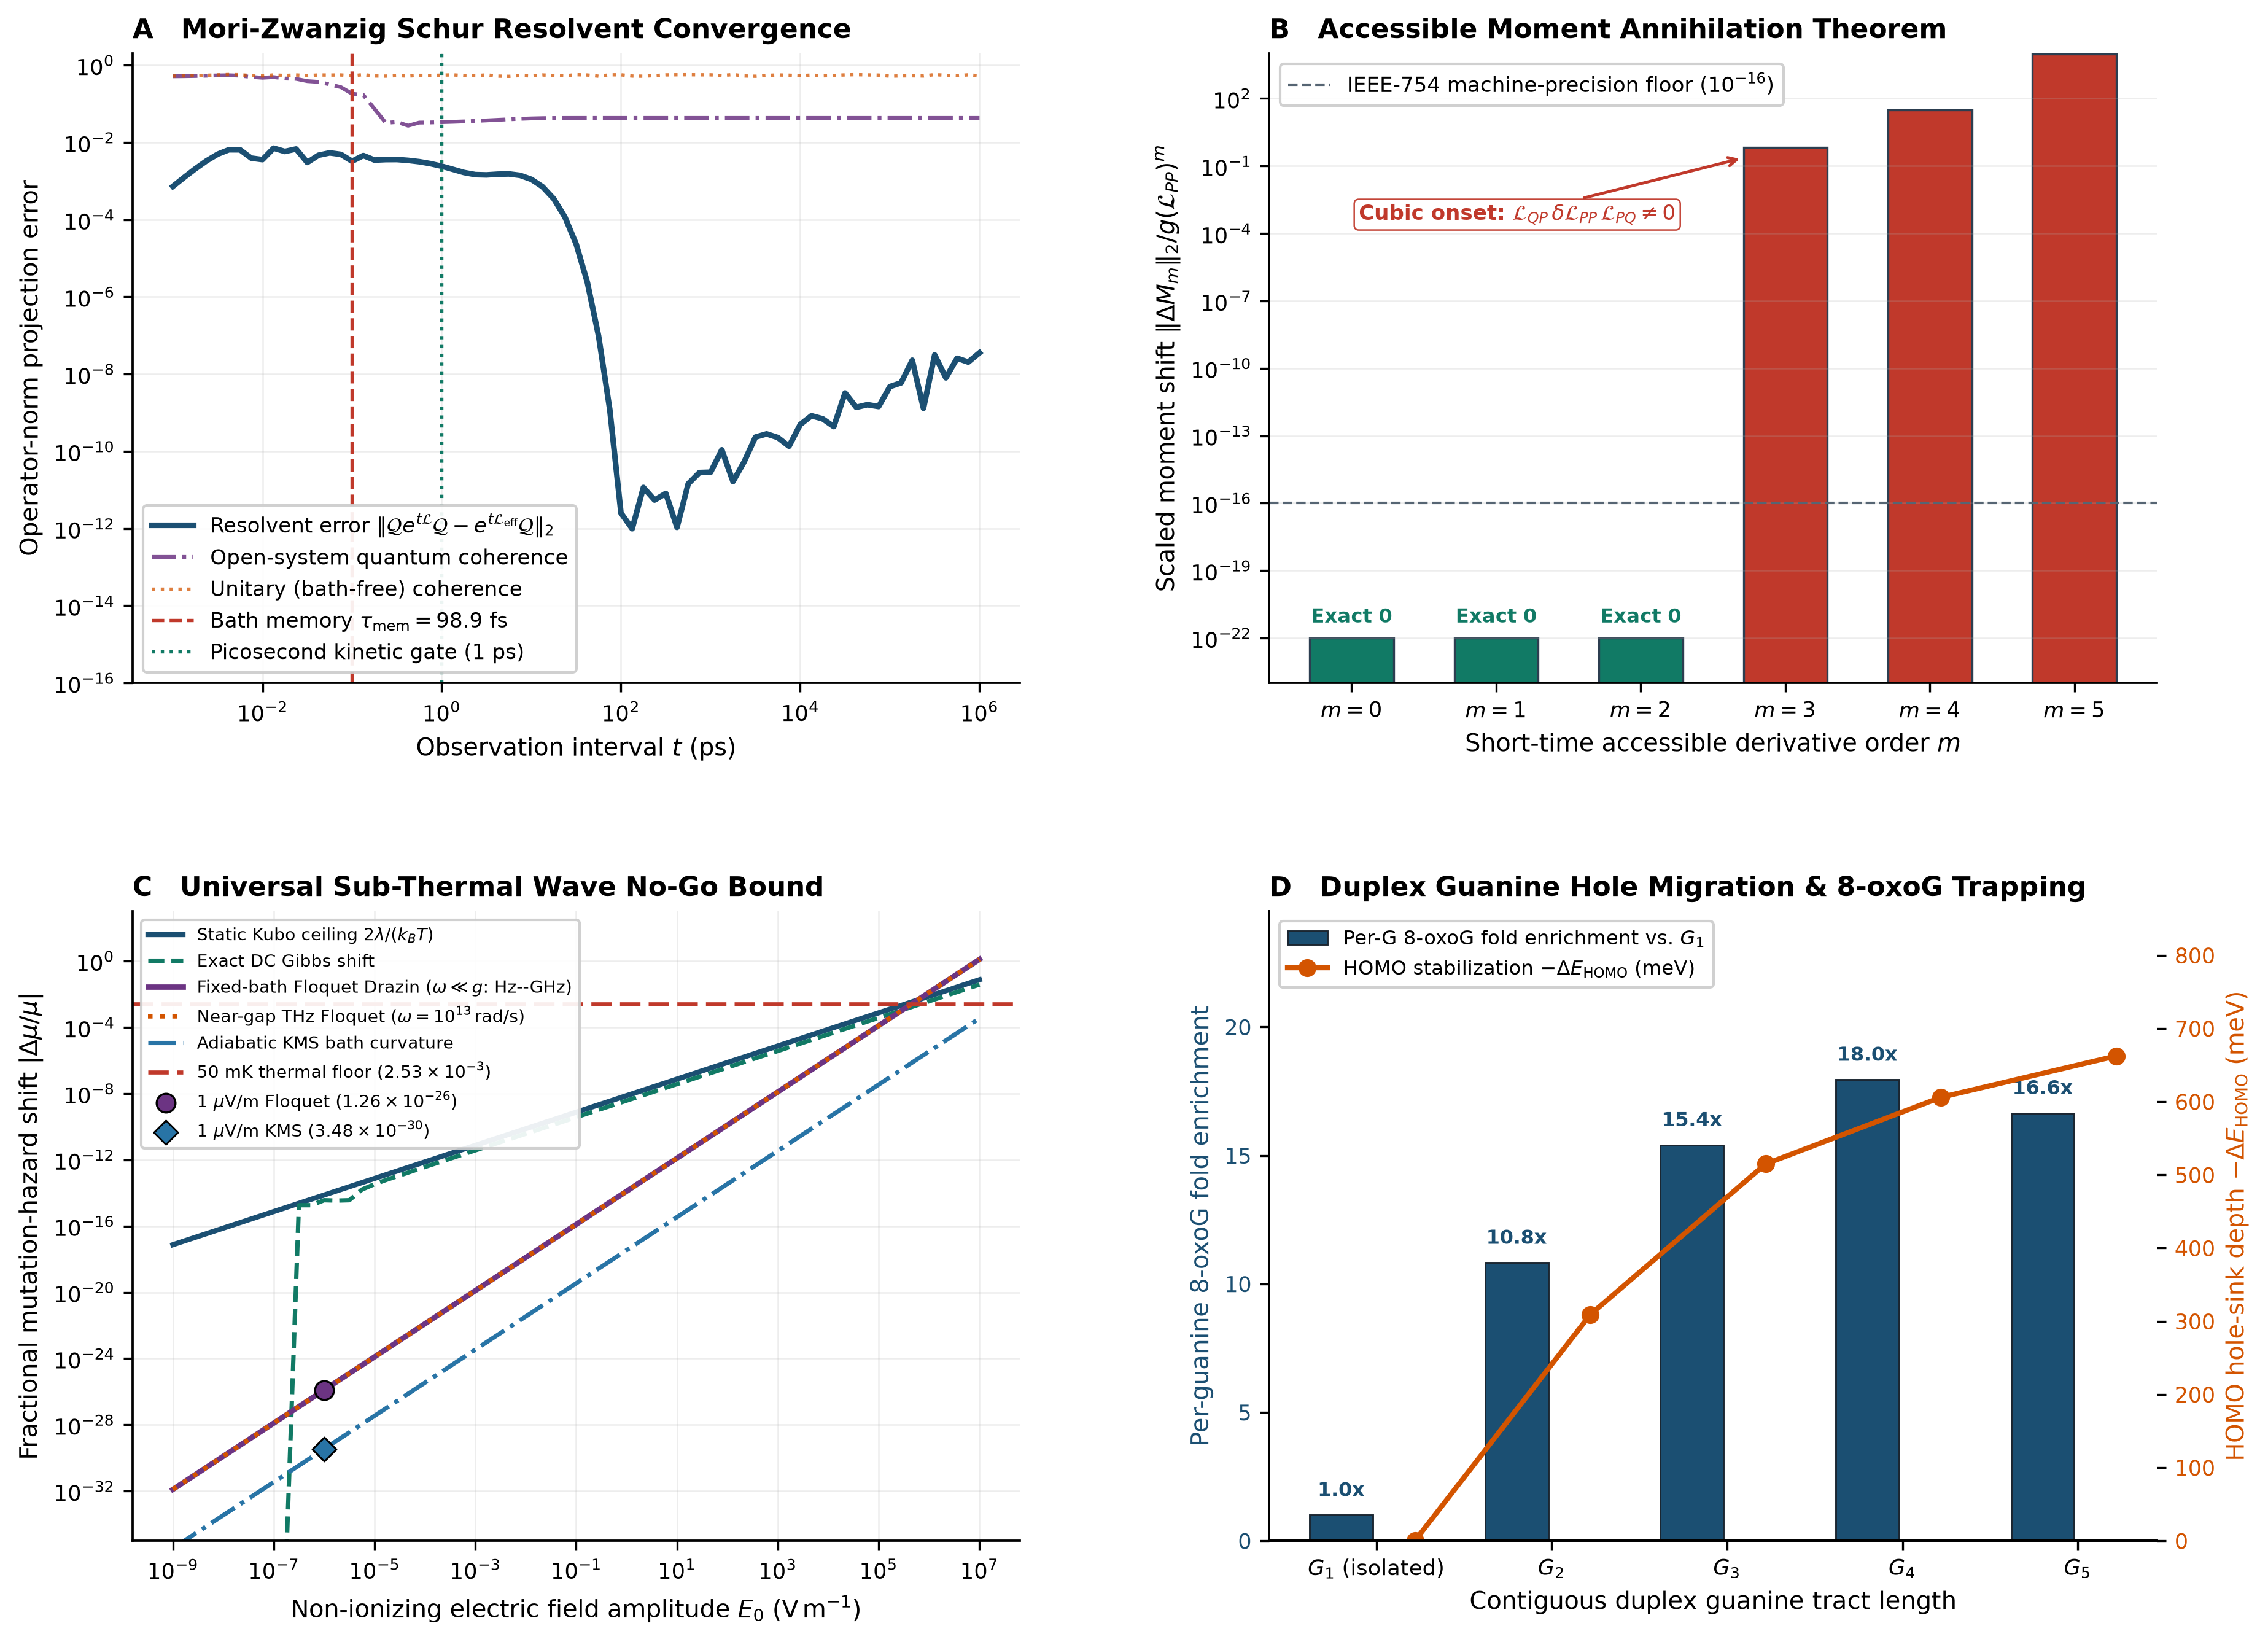
\includegraphics[width=0.98\textwidth]{assets/fig1_resolvent_and_nogo.png}
    \caption{\textbf{Mori--Zwanzig Schur resolvent projection, accessible moment annihilation, universal sub-thermal weak-field no-go bound, and duplex guanine hole-sink trapping.} \textbf{(A)} Operator-norm error $\|\Qcal e^{t\Lcal}\Qcal - e^{t\Lcal_{\mathrm{eff}}}\Qcal\|_2$ across observation intervals $t \in [1\,\mathrm{fs}, 1\,\mu\mathrm{s}]$ alongside open-system versus bath-free quantum coherence norms ($\tau_{\mathrm{mem}} = 98.9\,\mathrm{fs}$, coercivity $g_2(\Lcal_{PP}) = 1.009 \times 10^{13}\,\mathrm{s}^{-1}$). \textbf{(B)} Empirical verification of Theorem~\ref{thm:moment}: hidden-sector perturbations $\delta\Lcal_{PP}$ produce exact machine-zero changes in accessible derivatives $m=0,1,2$ and enter only at cubic order $m=3$ ($\|\Delta M_3\|_2 = 7.00 \times 10^{38}\,\mathrm{s}^{-3}$, matching Eq.~\eqref{eq:cubic_onset} to relative error $2.65 \times 10^{-14}$). \textbf{(C)} Fractional mutational hazard shift $|\Delta\mu/\mu|$ across ambient electric fields $E_0 \in [10^{-9}, 10^7]\,\mathrm{V\,m^{-1}}$ showing the static Kubo ceiling $2\lambda/(k_B T)$, exact DC Gibbs shift, fixed-dissipator Floquet--Lindblad Drazin shift ($\mathrm{Hz}$--$\mathrm{GHz}$ and near-gap $\omega = 10^{13}\,\mathrm{rad\,s^{-1}}$), and adiabatic KMS instantaneous-bath curvature relative to a $50\,\mathrm{mK}$ metabolic thermal floor ($2.53 \times 10^{-3}$). At $E_0 = 1\,\mu\mathrm{V\,m^{-1}}$ \cite{garcia2026dna}, $|\overline{\Delta\mu_{\mathrm{Floquet}}}/\mu_0| = 1.26 \times 10^{-26}$ and $|\overline{\Delta\mu_{\mathrm{KMS}}}/\mu_0| = 3.48 \times 10^{-30}$. \textbf{(D)} Tight-binding duplex hole migration across $\mathrm{G}_1$--$\mathrm{G}_5$ tracts showing HOMO stabilization $-\Delta E_{\mathrm{HOMO}}$ (orange) and per-guanine $\oxog$ quantum yield enrichment (navy, peaking at $18.0\times$ in $\mathrm{G}_4$).}
    \label{fig:fig1}
\end{figure}

Perturbing the fast coherence/tautomer block $\Lcal_{PP} \mapsto \Lcal_{PP} + \delta\Lcal_{PP}$ numerically confirms Theorem~\ref{thm:moment} (Fig.~\ref{fig:fig1}B): the zeroth, first, and second short-time accessible trajectory derivatives vanish identically ($\|\Delta M_0\|_2 = \|\Delta M_1\|_2 = \|\Delta M_2\|_2 = 0.0$), and hidden-sector structure emerges strictly at cubic order ($\|\Delta M_3\|_2 = 7.00 \times 10^{38}\,\mathrm{s}^{-3}$, matching the analytical sandwich product $\|\Lcal_{QP}(\delta\Lcal_{PP})\Lcal_{PQ}\|_2$ to relative error $2.65 \times 10^{-14}$). Consequently, short-time survival probabilities are quadratically insensitive to hidden-sector dephasing details, and any two microscopic Hamiltonians sharing the static Schur invariant $\Lcal_{QP}\Lcal_{PP}^{-1}\Lcal_{PQ}$ remain strictly non-identifiable across cellular replication windows.

\begin{table}[!t]
\centering
\caption{\textbf{Microscopic open-quantum parameters, universal sub-thermal weak-field perturbation limits, and duplex guanine hole-sink $\oxog$ yields (Module~1).} Perturbation bounds evaluated at $T = 310.15\,\mathrm{K}$ ($k_B T = 0.02673\,\mathrm{eV}$) across fixed-dissipator Floquet--Lindblad Drazin and adiabatic KMS bath regimes at reference amplitude $E_0 = 1\,\mu\mathrm{V\,m^{-1}}$ ($d_{\mathrm{eff}} = 1.0\,\text{\AA}$) \cite{garcia2026dna}.}
\label{tab:mod1}
\resizebox{\textwidth}{!}{%
\begin{tabular}{@{}llrr@{}}
\toprule
\textbf{Subsystem / Tract} & \textbf{Physical Observable or Metric} & \textbf{Computed Value} & \textbf{Reference / Comparison Scale} \\
\midrule
G:C KMS Liouvillian & Spectral gap $g(\Lcal_{PP})$ / coercivity $g_2(\Lcal_{PP})$ & $1.011$ / $1.009 \times 10^{13}\,\mathrm{s}^{-1}$ ($98.91\,\mathrm{fs}$) & $\kappa_2(V) = 1.00009$; $k_{\mathrm{pol}} \approx 10^3\,\mathrm{s}^{-1}$ \\
G:C KMS Liouvillian & Gibbs stationarity error $\|\rho_{\mathrm{ss}} - \rho_{\mathrm{Gibbs}}\|_F$ & $1.61 \times 10^{-11}$ & Eigenstate $p(E_1) = 1.46 \times 10^{-7}$ \\
Schur Resolvent & Semigroup error at $t = 1\,\mathrm{ps}$ / $t = 1\,\mathrm{ns}$ & $2.42 \times 10^{-3}$ / $2.88 \times 10^{-11}$ & $\|\Delta M_{0,1,2}\|_2 = 0$ (exact) \\
Sub-gap AC, $1\,\mu\mathrm{V\,m^{-1}}$ & Coupling $\lambda$ / Static ceiling $2\lambda/(k_B T)$ & $1.00 \times 10^{-16}\,\mathrm{eV}$ / $7.48 \times 10^{-15}$ & $50\,\mathrm{mK}$ floor $= 2.53 \times 10^{-3}$ \\
Sub-gap AC, $1\,\mu\mathrm{V\,m^{-1}}$ & Fixed-bath Floquet Drazin / Adiabatic KMS shift & $1.26 \times 10^{-26}$ / $3.48 \times 10^{-30}$ & Cohort ($10^5$ SNPs) $\mathrm{SNR} \le 3.99 \times 10^{-24}$ \\
\midrule
Duplex $\mathrm{G}_1$ (isolated) & $\Delta E_{\mathrm{HOMO}} = 0.000\,\mathrm{eV}$; mean $\Phi_{\oxog}/\mathrm{G}$ & $1.54 \times 10^{-3}$ ($1.00\times$) & Window capture $= 14.29\%$ \\
Duplex $\mathrm{G}_2$ (\texttt{GG}) & $\Delta E_{\mathrm{HOMO}} = -0.309\,\mathrm{eV}$; mean $\Phi_{\oxog}/\mathrm{G}$ & $1.66 \times 10^{-2}$ ($10.83\times$) & Window capture $= 82.60\%$ \\
Duplex $\mathrm{G}_3$ (\texttt{GGG}) & $\Delta E_{\mathrm{HOMO}} = -0.515\,\mathrm{eV}$; mean $\Phi_{\oxog}/\mathrm{G}$ & $2.37 \times 10^{-2}$ ($15.40\times$) & Window capture $= 91.61\%$ \\
Duplex $\mathrm{G}_4$ (\texttt{GGGG}) & $\Delta E_{\mathrm{HOMO}} = -0.606\,\mathrm{eV}$; mean $\Phi_{\oxog}/\mathrm{G}$ & $2.76 \times 10^{-2}$ ($17.95\times$) & Window capture $= 95.66\%$ \\
Duplex $\mathrm{G}_5$ (\texttt{GGGGG}) & $\Delta E_{\mathrm{HOMO}} = -0.662\,\mathrm{eV}$; mean $\Phi_{\oxog}/\mathrm{G}$ & $2.56 \times 10^{-2}$ ($16.65\times$) & Window capture $= 96.63\%$ \\
\bottomrule
\end{tabular}%
}
\end{table}

Evaluating Theorem~\ref{thm:nogo} across $16$ decades of electric-field amplitude $E_0 \in [10^{-9}, 10^7]\,\mathrm{V\,m^{-1}}$ establishes a rigorous ceiling for sub-thermal electromagnetic timing hypotheses \cite{garcia2026dna} across both open-quantum bath regimes (Fig.~\ref{fig:fig1}C and Table~\ref{tab:mod1}). For a $1.0\,\text{\AA}$ protonic displacement dipole at $E_0 = 10^{-6}\,\mathrm{V\,m^{-1}}$, the coupling is $\lambda = 1.00 \times 10^{-16}\,\mathrm{eV}$, bounding even an optimal static DC response to $|\Delta\mu_{\mathrm{DC}}/\mu_0| \le 7.48 \times 10^{-15}$ (exact Gibbs shift $3.63 \times 10^{-15}$, cohort $\mathrm{SNR} = 1.15 \times 10^{-12}$). For \emph{any} zero-mean oscillatory drive ($\mathrm{Hz}$ through $\mathrm{GHz}$ and near-gap $\omega = 10^{13}\,\mathrm{rad\,s^{-1}}$), first-order oscillations average to zero over millisecond polymerase steps: the exact fixed-dissipator Floquet--Lindblad Drazin shift evaluates to $|\overline{\Delta\mu_{\mathrm{Floquet}}}/\mu_0| = 1.26 \times 10^{-26}$ ($1.263 \times 10^{-26}$ sub-gap, $1.264 \times 10^{-26}$ near-gap; cohort $\mathrm{SNR} = 3.99 \times 10^{-24}$ across $M_0 = 10^5$ mutations; $50\,\mathrm{mK}$ crossover $E_0 \approx 4.48 \times 10^5\,\mathrm{V\,m^{-1}}$), while the instantaneously dressed adiabatic KMS bath shift collapses to $|\overline{\Delta\mu_{\mathrm{KMS}}}/\mu_0| = 3.48 \times 10^{-30}$ ($50\,\mathrm{mK}$ crossover $E_0 \approx 2.70 \times 10^7\,\mathrm{V\,m^{-1}}$)---$23$ to $27$ orders of magnitude below the $2.53 \times 10^{-3}$ Arrhenius rate shift of a $50\,\mathrm{mK}$ intracellular metabolic temperature fluctuation.

In sharp contrast to sub-thermal external fields, \emph{intrinsic} sequence-dependent quantum electronic structure exerts an order-of-magnitude effect at $310.15\,\mathrm{K}$ via radical-cation hole funneling \cite{rokhlenko2014jacs,rooman2014ioniz}. Across 21-bp duplex windows (Fig.~\ref{fig:fig1}D and Table~\ref{tab:mod1}), HOMO stabilization in contiguous guanine stacks elevates mean per-guanine $\oxog$ quantum yield $10.83$-fold in $\mathrm{GG}$ ($\Delta E_{\mathrm{HOMO}} = -0.309\,\mathrm{eV}$), $15.40$-fold in $\mathrm{GGG}$ ($-0.515\,\mathrm{eV}$), $17.95$-fold in $\mathrm{G}_4$ ($-0.606\,\mathrm{eV}$), and $16.65$-fold in $\mathrm{G}_5$ ($-0.662\,\mathrm{eV}$), concentrating $91.6\%$--$96.6\%$ of all duplex-window oxidative trapping events onto a single oligo-guanine motif.

\subsection*{Single-cell Poisson erasure versus ensemble van Trees--Clarke--Barron scaling in circadian OGG1-BER}

Having established that $\oxog$ deposition is strongly funneled into oligo-guanine promoter motifs, I next asked whether circadian OGG1 base-excision repair can transduce continuous $24\,\mathrm{h}$/$12\,\mathrm{h}$/$8\,\mathrm{h}$ metabolic redox waveforms into faithful promoter signaling records \cite{obermann2024redox,hahm2022emm,wang2025jbiomedsci}. Evaluating Proposition~\ref{prop:erasure} for a GC-rich mammalian core promoter ($K_{\mathrm{eff}} = 400$ guanines) at empirical steady-state $\oxog$ levels ($\bar{p}_{\oxog} \in \{10^{-6}, 3\times 10^{-6}, 10^{-5}\}$ per G) reveals a severe single-cell sparsity bottleneck: the expected lesion count per promoter per cell is $\lambda_{\mathrm{cell}} = 4.0 \times 10^{-4}$ to $4.0 \times 10^{-3}$, so $99.60\%$--$99.96\%$ of individual cells carry \emph{zero} $\oxog$ lesions at a given promoter ($P(N_{\mathrm{lesion}}=0) = 0.9996, 0.9988, 0.9960$), capping instantaneous single-cell mutual information at $9.35 \times 10^{-6}$ to $9.35 \times 10^{-5}\,\mathrm{bits}$ (Fig.~\ref{fig:fig2}A). Even integrated across $72\,\mathrm{h}$ of continuous OGG1 surveillance ($M=24$ bins of $3\,\mathrm{h}$, $K=6$ Fourier parameters, $N_{\mathrm{MC}} = 2{,}500$), a single cell ($\nu = 1$) exhibits $99.77\%$ empty $3\,\mathrm{h}$ bins, mutual information $I(\Theta; Y_1) = 4.68 \times 10^{-3}\,\mathrm{bits}$, and normalized waveform reconstruction MSE $D/\sigma_X^2 = 1.002 \pm 0.011$ (indistinguishable from prior-mean guessing, exact van Trees bound $0.999$). Single-cell promoter $\oxog$ occupancy is therefore an extreme Poisson erasure channel rather than a high-precision analog sensor.

\begin{figure}[!t]
    \centering
    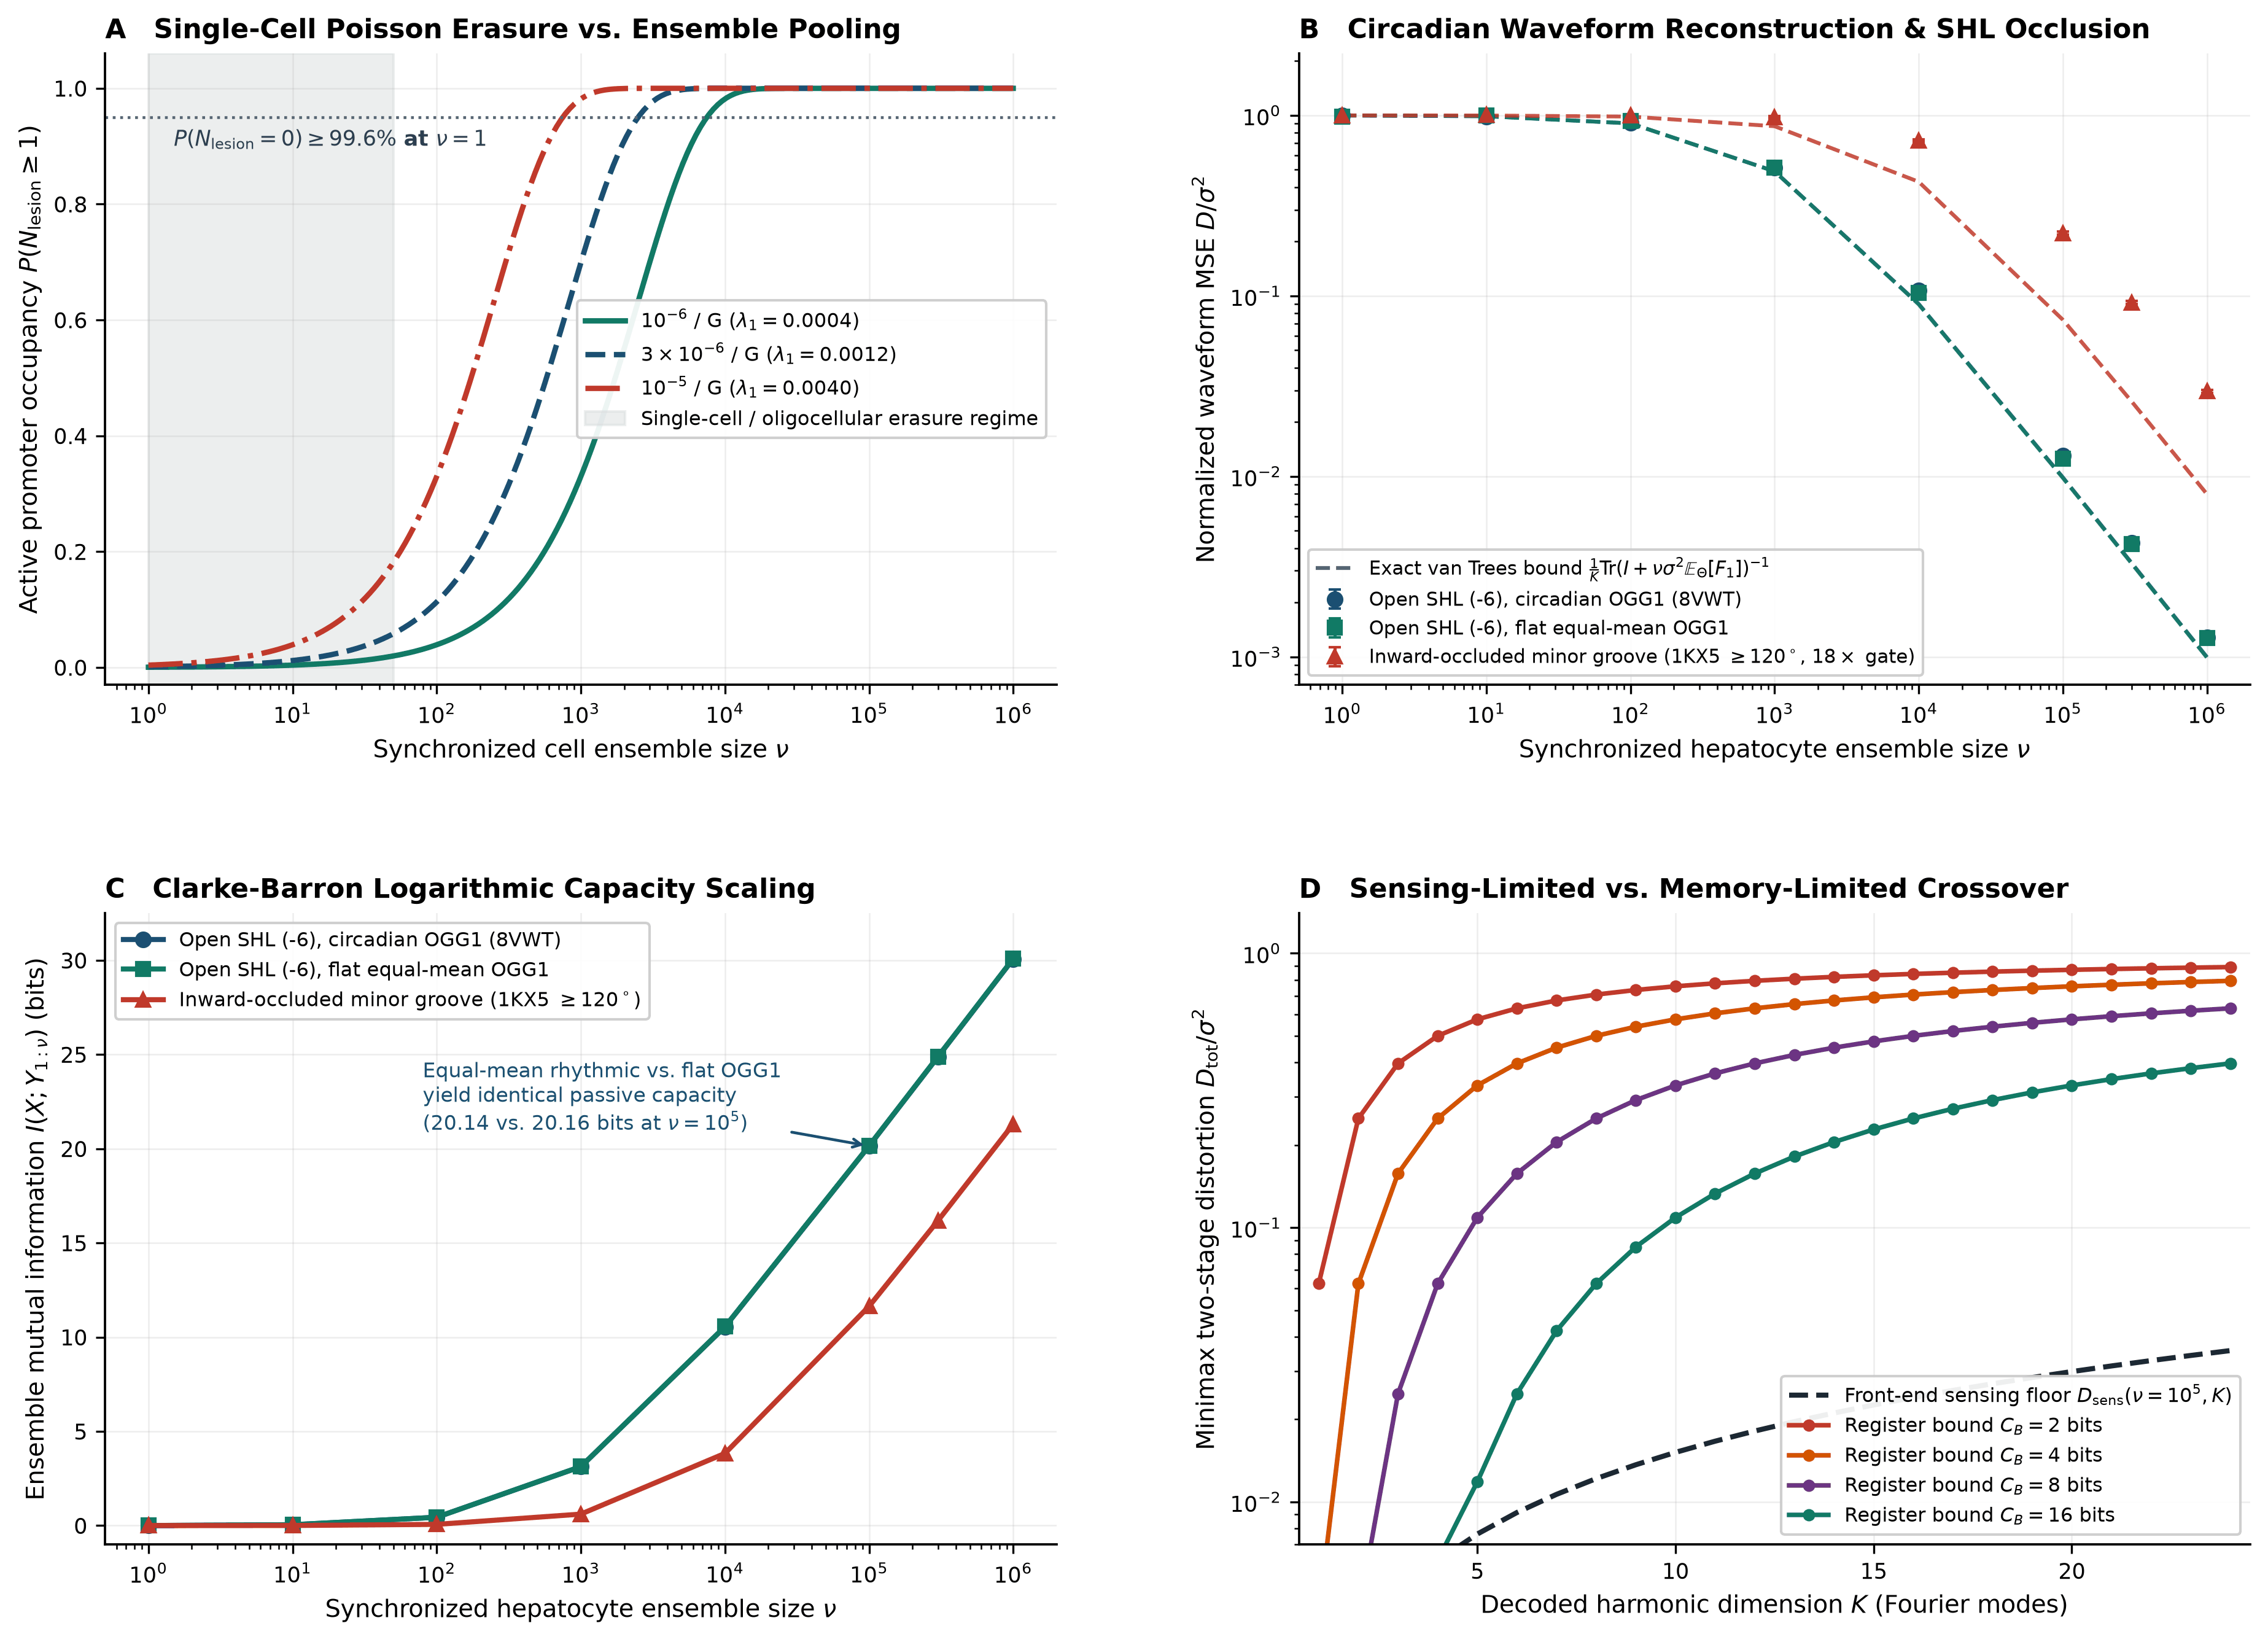
\includegraphics[width=0.98\textwidth]{assets/fig2_circadian_rate_distortion.png}
    \caption{\textbf{Single-cell Poisson erasure, distributed van Trees--Clarke--Barron scaling, nucleosomal occlusion, and classical-register crossover in circadian OGG1-BER.} \textbf{(A)} Active promoter lesion occupancy $P(N_{\mathrm{lesion}} \ge 1)$ versus synchronized cell ensemble size $\nu \in [1, 10^6]$ across physiological steady-state $\oxog$ fractions ($10^{-6}$ to $10^{-5}$ per G; $K_{\mathrm{eff}}=400\,\mathrm{G}$). \textbf{(B)} Empirical nonlinear Gauss--Newton Poisson MAP reconstruction distortion $D/\sigma_X^2$ ($\pm\,\mathrm{SEM}$, $N_{\mathrm{MC}}=2{,}500$) versus exact prior-averaged van Trees bounds (dashed curves, Eq.~\eqref{eq:twostage}, $N_{\mathrm{prior}}=5{,}000$) for solvent-exposed \texttt{SHL -6} (\texttt{8VWT}, circadian vs.\ flat equal-mean OGG1) and inward-occluded minor grooves ($\theta_{\mathrm{in}} \ge 120^\circ$ in \texttt{1KX5}, $K_{\mathrm{open}} = 0.08$). \textbf{(C)} Logarithmic growth of ensemble mutual information $I(X; Y_{1:\nu})$ across $\nu$, showing identical passive Fisher capacity for equal-mean rhythmic ($20.14\,\mathrm{bits}$) and flat ($20.16\,\mathrm{bits}$) OGG1 at $\nu = 10^5$. \textbf{(D)} Two-stage minimax distortion $D_{\mathrm{tot}}/\sigma_X^2 = \max\{D_{\mathrm{sens}}(\nu=10^5, K)/\sigma_X^2,\, 2^{-2C_B/K}\}$ across harmonic dimension $K \in [1, 24]$ for downstream classical register capacities $C_B \in \{2,4,8,16\}\,\mathrm{bits}$.}
    \label{fig:fig2}
\end{figure}

When synchronized across a multicellular tissue ensemble such as $10^4$--$10^6$ circadian-coupled hepatocytes, however, pooled BER excision fluxes overcome single-cell erasure strictly above the non-asymptotic van Trees bound of Theorem~\ref{thm:rd} across every ensemble scale (Fig.~\ref{fig:fig2}B,C and table~S1; accounting for exponential convexity $\exp(\frac{1}{2}\sigma_X^2)$ elevates $\Tr\overline{F}_1$ $1.152$-fold above origin linearization $\Tr F_1(0)$). For solvent-exposed nucleosomal DNA (\texttt{SHL -6}, PDB \texttt{8VWT} \cite{cordero2024natcommun}), normalized MAP distortion falls from $0.911 \pm 0.010$ at $\nu = 10^2$ (van Trees bound $0.903$; $0.443\,\mathrm{bits}$) and $0.515 \pm 0.006$ at $\nu = 10^3$ (van Trees bound $0.491$; $3.13\,\mathrm{bits}$) to $0.107 \pm 0.001$ at $\nu = 10^4$ (bound $0.090$; $10.55\,\mathrm{bits}$), $0.0130 \pm 0.0002$ at $\nu = 10^5$ (bound $0.0099$; $20.14\,\mathrm{bits}$), and $0.00128 \pm 0.00002$ at $\nu = 10^6$ (bound $0.00100$; $30.07\,\mathrm{bits}$). Two mechanistically decisive insights emerge from Fig.~\ref{fig:fig2}B--D:
\begin{enumerate}[leftmargin=1.8em,itemsep=2pt]
    \item \textbf{Chromatin Rotational Occlusion vs.\ Enzyme Oscillation:} Rotating the target guanine tract into an inward-facing histone-occluded minor groove ($K_{\mathrm{open}} = 0.08$, $\theta_{\mathrm{in}} \ge 120^\circ$ in \texttt{1KX5} \cite{cordero2024natcommun,ren2024natcommun}) degrades ensemble mutual information from $20.14$ to $11.64\,\mathrm{bits}$ at $\nu = 10^5$ and inflates empirical waveform reconstruction error \textbf{$17.1$-fold} ($D/\sigma_X^2 = 0.223$ vs.\ $0.0130$; van Trees bound $0.0737$ vs.\ $0.0099$). Conversely, holding mean enzyme abundance constant, circadian-oscillating OGG1 and flat OGG1 achieve virtually identical passive Fisher capacity ($20.14$ vs.\ $20.16\,\mathrm{bits}$; $D/\sigma_X^2 = 0.0130$ vs.\ $0.0126$ at $\nu = 10^5$). Thus, rhythmic OGG1 expression is not an information-maximizing passive receiver filter; rather, its physiological advantage lies in phase-locking excision repair to peak oxidative stress and S-phase/transcriptional vulnerability windows.
    \item \textbf{Classical-Register Rate-Distortion Bottleneck:} Even at $\nu = 10^5$ hepatocytes where front-end BER sensing error is low ($D_{\mathrm{sens}}/\sigma_X^2 = 0.0092$ at $K=6$), compressing the trajectory into a finite downstream transcriptional or chromatin state of capacity $C_B \in \{2, 4, 8, 16\}\,\mathrm{bits}$ triggers hard sensing-to-memory crossovers at $K^*(C_B) = 1, 1, 2, 5$ harmonic modes, respectively (Fig.~\ref{fig:fig2}D). For a binary or quaternary enhancer state ($C_B = 2$--$4\,\mathrm{bits}$), multi-harmonic circadian reconstruction is strictly memory-limited ($D_{\mathrm{mem}}/\sigma_X^2 = 0.630$ and $0.397$ at $K=6$) regardless of further increases in cell number $\nu$.
\end{enumerate}


\subsection*{Empirical uncollapsing of mutational quotients across 27 \emph{Escherichia coli} genomes}

To test whether genetic ablation of intermediate enzymatic gates $\Phi_{\mathrm{gate}}$ uncollapses distinct pre-repair molecular error spectra in living organisms, I analyzed $10{,}467$ unique single-base substitutions across all $27$ independent \emph{E.\ coli} \texttt{REL606} populations from the $50{,}000$-generation LTEE and $13{,}750$-generation MAE datasets \cite{tenaillon2016nature} (Fig.~\ref{fig:fig3} and Table~\ref{tab:mod3}). In the $n = 20$ repair-proficient wild-type populations ($471$ unique SNPs), coupled Pol~III proofreading, MutS/MutL/MutH mismatch repair, and GO-system (\emph{mutT}/\emph{mutM}/\emph{mutY}) surveillance equalize residual error modes into a high-entropy quotient on $\Delta^{95}$ (opportunity-normalized Shannon entropy $H = 6.073\,\mathrm{bits}$; pooled transition fraction $50.96\%$; per-lineage transition mean $\pm\,\mathrm{SD} = 47.36\% \pm 15.07\%$; Fig.~\ref{fig:fig3}A).

\begin{figure}[!t]
    \centering
    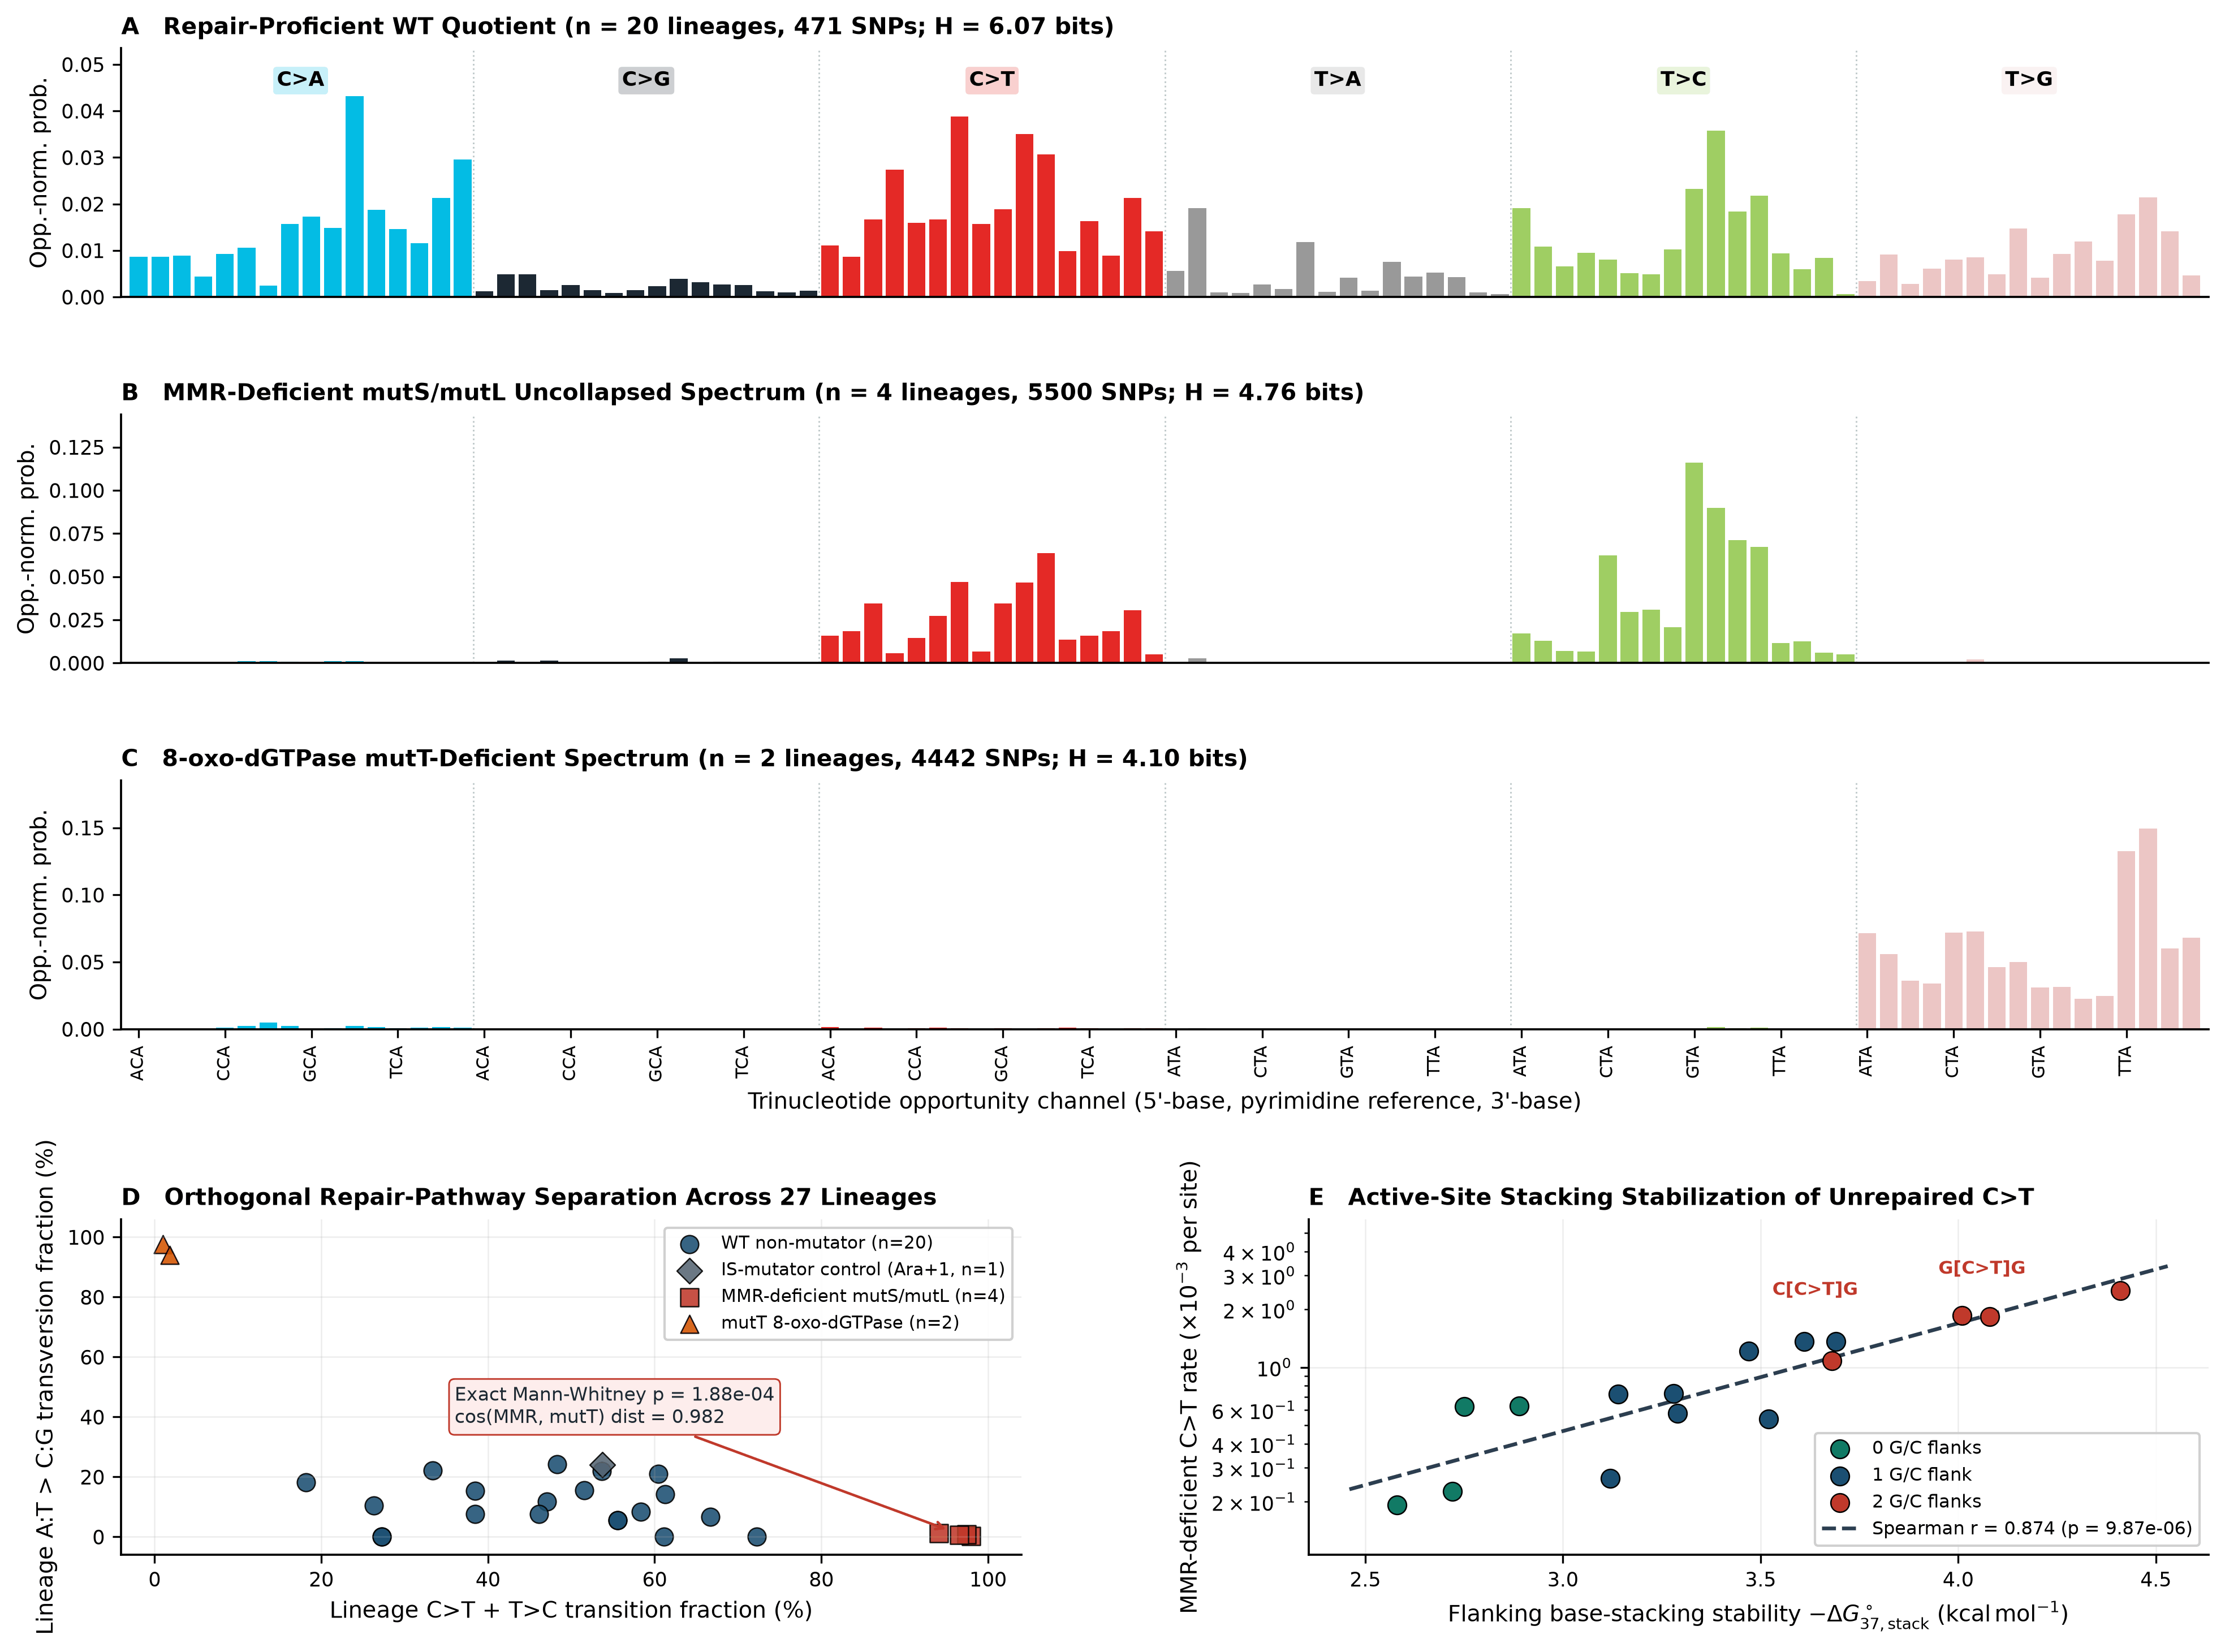
\includegraphics[width=0.98\textwidth]{assets/fig3_ecoli_quotient_uncollapsing.png}
    \caption{\textbf{Empirical observational quotient uncollapsing across 27 independent \emph{Escherichia coli} \texttt{REL606} populations and active-site base-stacking thermodynamics.} \textbf{(A--C)} Trinucleotide-opportunity-normalized SBS-96 mutational probability profiles on $\Delta^{95}$ for \textbf{(A)} repair-proficient wild-type lineages ($n=20$, $H = 6.07\,\mathrm{bits}$), \textbf{(B)} MutS/MutL mismatch-repair-deficient hypermutators ($n=4$, $5{,}500$ SNPs, $H = 4.76\,\mathrm{bits}$), and \textbf{(C)} \emph{mutT} 8-oxo-dGTPase-deficient hypermutators ($n=2$, $4{,}442$ SNPs, $H = 4.10\,\mathrm{bits}$). \textbf{(D)} Complete separation of all $27$ independent populations in the $(\mathrm{C{>}T}+\mathrm{T{>}C},\, \mathrm{A{:}T{>}C{:}G})$ simplex plane (exact two-sided Mann--Whitney $p = 1.88 \times 10^{-4}$ for WT vs.\ MMR transitions; $\cos(\mathrm{MMR},\mathrm{mutT})$ distance $= 0.982$). \textbf{(E)} Across all $16$ $\mathrm{C{>}T}$ trinucleotide contexts in MMR-deficient genomes, site-normalized mutation rates correlate strongly with nearest-neighbor SantaLucia base-stacking stability $-\Delta G^\circ_{37,\mathrm{stack}}$ (Spearman $r = 0.874$, $p = 9.87 \times 10^{-6}$).}
    \label{fig:fig3}
\end{figure}

Inactivating MutS/MutL post-replicative mismatch repair ($n = 4$ independent populations: \texttt{Ara+3}, \texttt{Ara-2}, \texttt{Ara-3}, \texttt{Ara-4}; $5{,}500$ unique SNPs) dramatically compresses SBS-96 entropy by $\Delta H = -1.312\,\mathrm{bits}$ ($H = 4.761\,\mathrm{bits}$) onto unrepaired Pol~III replication transitions ($\mathrm{C{>}T}$ and $\mathrm{T{>}C}$; pooled transition fraction $96.89\%$; per-lineage mean $96.52\% \pm 1.71\%$, range $94.11\%$--$97.95\%$; exact two-sided Mann--Whitney $U$ $p = 1.88 \times 10^{-4}$ vs.\ WT; Fig.~\ref{fig:fig3}B,D). Equal-weight lineage-balanced permutation testing across all $24$ WT + MMR populations confirms highly significant divergence on the full 96-channel simplex (equal-weight Jensen--Shannon divergence $0.329\,\mathrm{bits}$, $p_{\mathrm{emp}} = 2.00 \times 10^{-4}$; cosine distance $0.396$, $p_{\mathrm{emp}} = 1.10 \times 10^{-3}$; pooled $D_{\mathrm{KL}}(\mathrm{MMR}\parallel\mathrm{WT}) = 1.144\,\mathrm{bits}$). Conversely, ablating the \emph{mutT} nudix hydrolase that sanitizes oxidized $\text{8-oxo-dGTP}$ from the nucleotide pool ($n = 2$ populations: \texttt{Ara-1}, \texttt{Ara+6}; $4{,}442$ unique SNPs) uncollapses an \emph{orthogonal} oxidative transversion channel ($96.65\%$ $\mathrm{A{:}T \to C{:}G}$ [$\mathrm{T{>}G}$], $H = 4.102\,\mathrm{bits}$), separated from the MMR-deficient spectrum by a cosine distance of \textbf{$0.9818$} ($D_{\text{JS}} = 0.8928\,\mathrm{bits}$; Fig.~\ref{fig:fig3}C,D). Meanwhile, the insertion-sequence mutator control (\texttt{Ara+1}, $54$ SNPs) retains a wild-type-like base-substitution transition fraction ($53.70\%$), confirming pathway specificity.

\begin{table}[!t]
\centering
\caption{\textbf{Empirical mutational quotient divergence across 27 independent \emph{E.\ coli} \texttt{REL606} experimental evolution populations (Module~3A).} Opportunity-normalized SBS-96 metrics, lineage-unit statistics, and flanking base-stacking correlation.}
\label{tab:mod3}
\resizebox{\textwidth}{!}{%
\begin{tabular}{@{}lrrrr@{}}
\toprule
\textbf{Genomic Regime} & \textbf{Lineages ($n$)} & \textbf{Unique SNPs} & \textbf{Lineage $\mathrm{C{>}T}+\mathrm{T{>}C}$ (\%)} & \textbf{SBS-96 $H$ (bits) / Divergence} \\
\midrule
WT repair-proficient & $20$ & $471$ & $47.36 \pm 15.07\%$ (pooled $51.0\%$) & $H = 6.073$ (reference quotient) \\
IS-mutator control (\texttt{Ara+1}) & $1$ & $54$ & $53.70\%$ ($\mathrm{A{:}T{>}C{:}G} = 24.1\%$) & Structural transposition control \\
MMR-deficient (\emph{mutS}/\emph{mutL}) & $4$ & $5{,}500$ & $96.52 \pm 1.71\%$ (pooled $96.9\%$) & $H = 4.761$; $p_{\mathrm{MWU}} = 1.88 \times 10^{-4}$ \\
\emph{mutT} 8-oxo-dGTPase mutator & $2$ & $4{,}442$ & $1.19\%$ ($\mathrm{A{:}T{>}C{:}G} = 96.65\%$) & $H = 4.102$; $\cos(\mathrm{MMR},\mathrm{mutT}) = 0.982$ \\
\midrule
\multicolumn{5}{@{}l}{\textbf{MMR vs.\ WT 96-Channel Tests:} Equal-weight lineage $D_{\mathrm{JS}} = 0.329\,\mathrm{bits}$ ($p_{\mathrm{emp}} = 2.00 \times 10^{-4}$); pooled $D_{\mathrm{KL}}(\mathrm{MMR}\parallel\mathrm{WT}) = 1.144\,\mathrm{bits}$.} \\
\multicolumn{5}{@{}l}{\textbf{MMR $\mathrm{C{>}T}$ Flanking Stacking ($16$ contexts):} Spearman $r = 0.8735$, $p = 9.87 \times 10^{-6}$ vs.\ $-\Delta G^\circ_{37,\mathrm{stack}}$ ($\mathrm{G[C{>}T]G}$ peak).} \\
\bottomrule
\end{tabular}%
}
\end{table}

Once MutS/MutL surveillance is removed, the uncollapsed $\mathrm{C{>}T}$ ($\mathrm{G{:}C \to A{:}T}$) transition rates across all $16$ trinucleotide contexts correlate strongly with nearest-neighbor SantaLucia base-stacking stability $-\Delta G^\circ_{37,\mathrm{stack}}$ (\textbf{Spearman $r = 0.8735$, $p = 9.87 \times 10^{-6}$}; Fig.~\ref{fig:fig3}E), rising nearly an order of magnitude from AT-flanked contexts (\texttt{A[C>T]A}, \texttt{T[C>T]A}) to GC-flanked contexts (\texttt{G[C>T]G}, \texttt{C[C>T]G}) \cite{lee2012pnas,foster2018genetics}. Stronger aromatic $\pi$-stacking from $5'$ and $3'$ G/C neighbors thermodynamically stabilizes transient wobble/tautomer/ionized $\mathrm{G}\cdot\mathrm{T}$ mispairs inside the polymerase active site against $3'\to 5'$ exonuclease fraying, demonstrating that microscopic local energetics directly govern pre-repair error channels that are masked in wild-type genomes. Comparing coding synonymous versus intergenic substitutions highlights an essential methodological control: raw synonymous-to-intergenic rate ratios shift from $0.55$ in WT MAE to $1.65$ in MMR-deficient LTEE because \texttt{REL606} coding regions are GC-enriched relative to intergenic DNA, whereas conditioning on exact 6-spectrum base opportunities contracts the MMR-deficient ratio to $1.15$.

\subsection*{Non-teleological structural inheritance in human clock promoters and AlphaGenome cis-regulatory distortion}

I next tested whether human core circadian clock promoters ($n = 10$ MANE Select promoters: \emph{BMAL1}, \emph{CLOCK}, \emph{CRY1}, \emph{CRY2}, \emph{DBP}, \emph{NPAS2}, \emph{NR1D1}, \emph{NR1D2}, \emph{PER1}, \emph{PER2}) evolved specialized $\oxog$ hole-trapping or 10.4-bp nucleosomal phasing architectures beyond general GC-rich CpG-island (CGI) promoters ($N_{\mathrm{ctrl}} = 1{,}500$ Mahalanobis propensity-matched human protein-coding CGI promoters drawn from $4{,}560$ non-clock MANE genes; Fig.~\ref{fig:fig4}A and table~S2). Relative to the unstratified genome-wide background ($4{,}560$ genes), the $10$ clock promoters are strongly enriched in GC content ($68.88\% \pm 5.38\%$ vs.\ $61.54\%$), CpG observed/expected ratio ($0.801 \pm 0.142$ vs.\ $0.614$), contiguous $\mathrm{G}_{\ge 3}$ runs ($59.4 \pm 10.4$ vs.\ $52.3$), $\oxog$ hole-trapping burden ($9.24 \pm 1.36$ vs.\ $7.98$), and $\mathrm{SP1}$ \texttt{GGGCGG} boxes ($5.00 \pm 2.58$ vs.\ $3.53$). Once propensity-matched against the $1{,}500$ CGI controls on GC\%, CpG O/E, maximum G-run length, and G4Hunter score ($|\Delta_{\mathrm{std}}| \le 0.302$ on all four covariates), however, \textbf{every downstream biophysical and cis-regulatory metric collapses into statistical equivalence} (all Benjamini--Hochberg $q = 0.820$): $\mathrm{G}_{\ge 3}$ tracts ($\Delta_{\mathrm{std}} = -0.227$, $p = 0.471$), integrated $\oxog$ hole-trapping burden ($\Delta_{\mathrm{std}} = +0.066$, $p = 0.806$), mean $\Phi_{\oxog}$ per G ($\Delta_{\mathrm{std}} = -0.136$, $p = 0.820$), and 10.4-bp rotational dinucleotide PSD ($\Delta_{\mathrm{std}} = -0.183$, $p = 0.410$). Mammalian circadian promoters therefore did not undergo teleological fine-tuning to become quantum redox antennas; rather, maintaining constitutively accessible, TATA-less CGI promoters rich in $\mathrm{SP1}$ (\texttt{GGGCGG}) and E-box (\texttt{CACGTG}) motifs \emph{structurally forces} dense oligo-guanine hole sinks as an unavoidable biophysical spandrel.

\begin{figure}[!t]
    \centering
    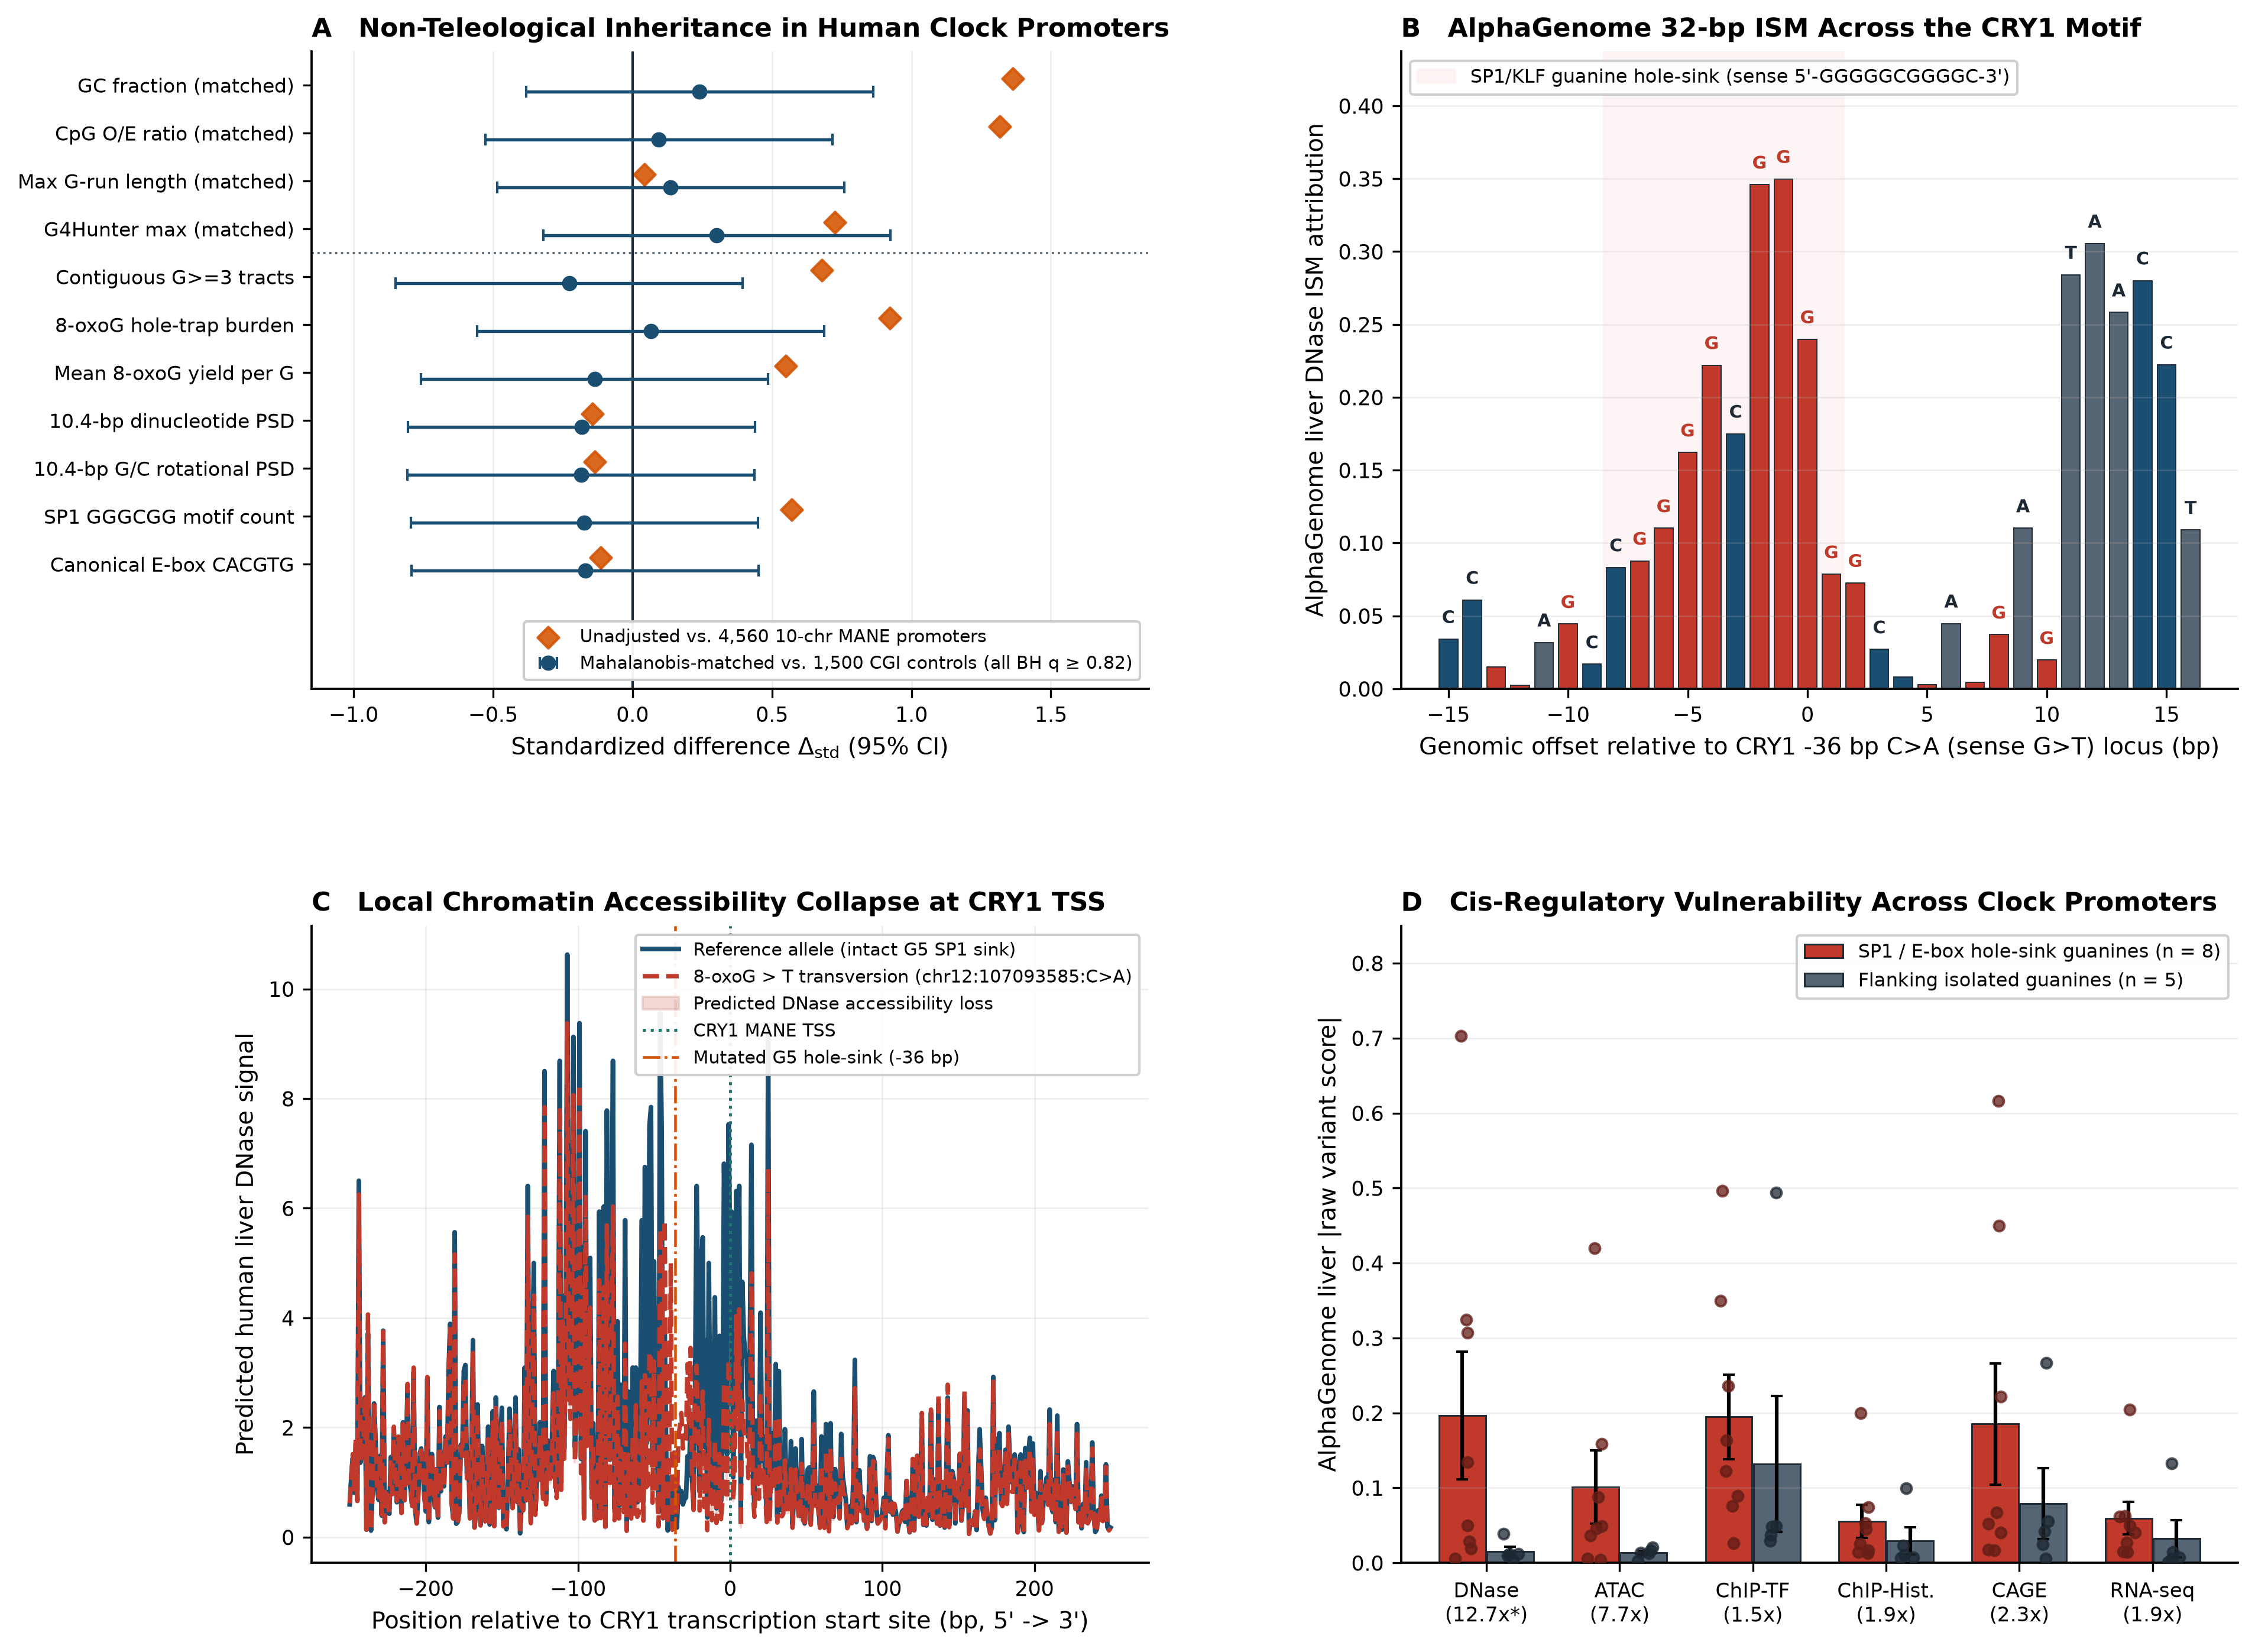
\includegraphics[width=0.98\textwidth]{assets/fig4_human_promoters_and_alphagenome.png}
    \caption{\textbf{Non-teleological structural inheritance across 1,500 matched human promoters and AlphaGenome 1-Mb-context regulatory disruption in human liver.} \textbf{(A)} Standardized differences $\Delta_{\mathrm{std}}$ ($95\%$ CI) comparing $10$ human core circadian promoters against $4{,}560$ genome-wide MANE promoters (amber diamonds) versus $1{,}500$ Mahalanobis propensity-matched CGI controls (navy circles; all outcome BH $q = 0.82$). \textbf{(B)} AlphaGenome human liver (\texttt{UBERON:0002107}) DNase \emph{in silico} mutagenesis (ISM) L2 attribution across the $32$-bp \emph{CRY1} core-promoter window centered at \texttt{chr12:107093585:C>A} ($-36\,\mathrm{bp}$ upstream of MANE TSS), resolving the sense \texttt{5'-GGGGGCGGGGC-3'} SP1/KLF hole sink and adjacent \texttt{CCAAT} box. \textbf{(C)} Base-resolution $\pm 250\,\mathrm{bp}$ predicted human liver DNase accessibility tracks for the reference allele versus the \texttt{chr12:107093585:C>A} ($\oxog \to \mathrm{T}$) transversion at the \emph{CRY1} TSS. \textbf{(D)} AlphaGenome human liver $|\text{raw variant score}|$ ($\mathrm{mean} \pm \mathrm{SEM}$ plus individual variants) across six regulatory modalities comparing $\oxog \to \mathrm{T}$ transversions inside $\mathrm{SP1}$/E-box guanine hole sinks ($n=8$) versus flanking isolated guanines ($n=5$) in \emph{CRY1}, \emph{PER1}, \emph{PER2}, and \emph{BMAL1} ($*p = 0.0295$ on ATAC).}
    \label{fig:fig4}
\end{figure}

What happens when unrepaired $\oxog$ lesions within those inherited promoter sinks mispair with adenine during replication or transcription-coupled synthesis to fix $\mathrm{G{:}C \to T{:}A}$ transversions? Applying 1-Mb-context AlphaGenome modeling in human liver (\texttt{UBERON:0002107}) reveals an acute coupling between quantum-chemical hole migration and cis-regulatory vulnerability (Fig.~\ref{fig:fig4}B--D and table~S2). At the \emph{CRY1} core promoter, 32-bp single-nucleotide ISM around $-36\,\mathrm{bp}$ (\texttt{chr12:107093585:C>A}) uncovers a sharply localized regulatory grammar pairing an upstream inverted \texttt{CCAAT} element with a high-attribution sense \texttt{5'-GGGGGCGGGGC-3'} $\mathrm{SP1}$/KLF $\mathrm{G}_5$ hole sink (top 8-mer \texttt{CCCCGCCC} / \texttt{GGGCGGGG}, attribution score $1.692$; Fig.~\ref{fig:fig4}B), where a single $\oxog \to \mathrm{T}$ transversion collapses predicted local DNase hypersensitivity across the \emph{CRY1} TSS (Fig.~\ref{fig:fig4}C). Across all $13$ \texttt{GRCh38}-verified $\oxog \to \mathrm{T}$ promoter transversions in \emph{CRY1}, \emph{PER1}, \emph{PER2}, and \emph{BMAL1}, mutations within $\mathrm{SP1}$/\texttt{CACGTG} guanine hole sinks ($n=8$) produce \textbf{$8.54$-fold larger mean $|\text{raw}|$ disruption on liver DNase} ($0.2016$ vs.\ $0.0236$; mean $|\text{quantile}| = 0.859$ vs.\ $0.539$), \textbf{$4.31$-fold larger disruption on liver ATAC} ($0.1281$ vs.\ $0.0297$, two-sided Mann--Whitney $p = 0.0295$; mean $|\text{quantile}| = 0.891$ vs.\ $0.590$), \textbf{$2.20$-fold larger disruption on histone ChIP} ($0.1131$ vs.\ $0.0514$, $p = 0.093$), and \textbf{$1.81$-fold larger disruption on exon RNA-seq} ($0.0710$ vs.\ $0.0392$) than $\oxog \to \mathrm{T}$ transversions at flanking isolated $G_1$ sites within the same promoters (Fig.~\ref{fig:fig4}D and table~S2). The single largest transcription-factor binding disruption occurs at the central guanine of the canonical \emph{PER1} $-170\,\mathrm{bp}$ \texttt{CACGTG} E-box (\texttt{chr17:8152574:C>A}, liver \texttt{CHIP\_TF} $\text{raw} = -0.9737$, $\text{quantile} = -0.999992$), while the largest chromatin accessibility losses occur in the \emph{CRY1} $-304\,\mathrm{bp}$ and $-34\,\mathrm{bp}$ and \emph{PER1} $-83\,\mathrm{bp}$ $\mathrm{SP1}$ $\mathrm{G}_5$ hole sinks ($\text{DNase quantiles} = -0.99958, -0.99089, -0.99230$).


\subsection*{Upgraded 300-kbp codebase audit, Earth--Sun chiral solar-neutrino quadrature, and 240,000-trajectory helical lepton funneling}

Finally, I executed a full algorithmic rewrite of the four exploratory quantum-DNA simulation families accompanying Ref.~\cite{garcia2026dna} across $2{,}000$ non-overlapping $150$-bp windows ($300\,\mathrm{kbp}$) of \emph{E.\ coli} \texttt{REL606} and evaluated how Earth--Sun astrodynamics couples chiral solar fusion neutrinos ($\nu_e$) versus Globus--Blandford weak-decay spin-polarized secondary leptons ($\pi^\pm \to \mu^\pm + \nu_\mu \to e^\pm$) \cite{globus2020apjl,globus2021apj,globus2021muons,appel2022borexino} to helical B-DNA (Fig.~\ref{fig:fig5} and Table~\ref{tab:mod5}). My codebase audit resolved four numerical artifacts in the baseline routines:
\begin{enumerate}[leftmargin=1.8em,itemsep=2pt]
    \item \textbf{Trace-Violation GC Artifact ($300\,\mathrm{kbp}$ Audit):} \texttt{Von\_\allowbreak Neumann\_\allowbreak entropy.py} mapped $\mathrm{C} \mapsto [1,1]^\top$ ($\|\psi\|^2 = 2$) and $\mathrm{G} \mapsto [0,0]^\top$ ($\|\psi\|^2 = 0$), violating $\Tr(\rho) = 1$ ($\Tr\rho = 0.920$ on the $200$-bp benchmark). Across $1{,}000$ coding CDS ($\overline{\mathrm{GC}} = 52.18\%$) versus $1{,}000$ intergenic $150$-bp windows ($\overline{\mathrm{GC}} = 42.60\%$) of \texttt{REL606}, this unnormalized mapping creates an inflated $0.0690$-bit gap ($S_{\mathrm{orig}} = 0.7940 \pm 0.0753$ vs.\ $0.8631 \pm 0.0803$, Mann--Whitney $p = 7.00 \times 10^{-76}$); enforcing trace-normalized Bloch states ($\Tr\rho = 1$) compresses that gap $67$-fold to $0.9932 \pm 0.0077$ vs.\ $0.9921 \pm 0.0080\,\mathrm{bits}$ ($p = 3.41 \times 10^{-4}$, reflecting true bacterial AT/GC skew; Fig.~\ref{fig:fig5}B), alongside repaired 2-qubit dinucleotide mutual information ($0.0720 \pm 0.0314$ vs.\ $0.0635 \pm 0.0309\,\mathrm{bits}$, $p = 4.44 \times 10^{-11}$) and $150 \times 150$ $\pi$-stack thermal $\mathrm{G}_{\ge 3}$ hole capture ($0.3473 \pm 0.2572$ vs.\ $0.3701 \pm 0.2995$, $p = 0.0172$).
    \item \textbf{Separable Product-State Construction:} \texttt{Entanglement\_\allowbreak Analysis} summed all $(q_1, q_2)$ outer products to form the exact separable product state $\rho_{12} = \rho_1 \otimes \rho_2$, yielding strictly zero entanglement (Peres--Horodecki negativity $\mathcal{N} = 0.0$, quantum mutual information $|I_Q| \le 8.88 \times 10^{-16}\,\mathrm{bits}$ across $100$ window pairs).
    \item \textbf{SI-to-Dimensionless Noise Mismatch:} \texttt{Mutations\_\allowbreak induction} added dimensionless noise $0.05$ directly to SI Joules ($\lambda = 1.60 \times 10^{-35}\,\mathrm{J} = 1.00 \times 10^{-16}\,\mathrm{eV}$ at $1\,\mu\mathrm{V\,m^{-1}}$), injecting $0.05\,\mathrm{J} = 3.12 \times 10^{17}\,\mathrm{eV}$ kicks ($3.12 \times 10^{33}\times$ larger than the dipole coupling) into a symmetric ($\Delta E = 0$) well; restoring KMS detailed balance ($\Delta E_{\mathrm{GC}} = 0.42\,\mathrm{eV}$, $\Delta E_{\mathrm{AT}} = 0.56\,\mathrm{eV}$, $310.15\,\mathrm{K}$) recovers physical tautomer hazards.
    \item \textbf{Forward-Euler Instability and Chirp Scaling:} \texttt{Quantum\_\allowbreak state\_\allowbreak evolution} used forward Euler in the numerically unstable regime ($\|H\|\,\mathrm{d}t/\hbar = 12.15 \gg 1$) and injected asymmetric frequency chirps; under an exact matrix-exponential propagator ($e^{-iHt/\hbar}$) with symmetric $1\,\mu\mathrm{V\,m^{-1}}$ coupling, $\|U_{\mathrm{ext}} - U_0\|_2 = 5.14 \times 10^{-11}$ at $1\,\mathrm{ps}$, and Earth's diurnal rotational fractional Doppler chirp is $|\dot{f}/f_0| = 1.13 \times 10^{-10}\,\mathrm{s}^{-1}$.
\end{enumerate}

\begin{figure}[!t]
    \centering
    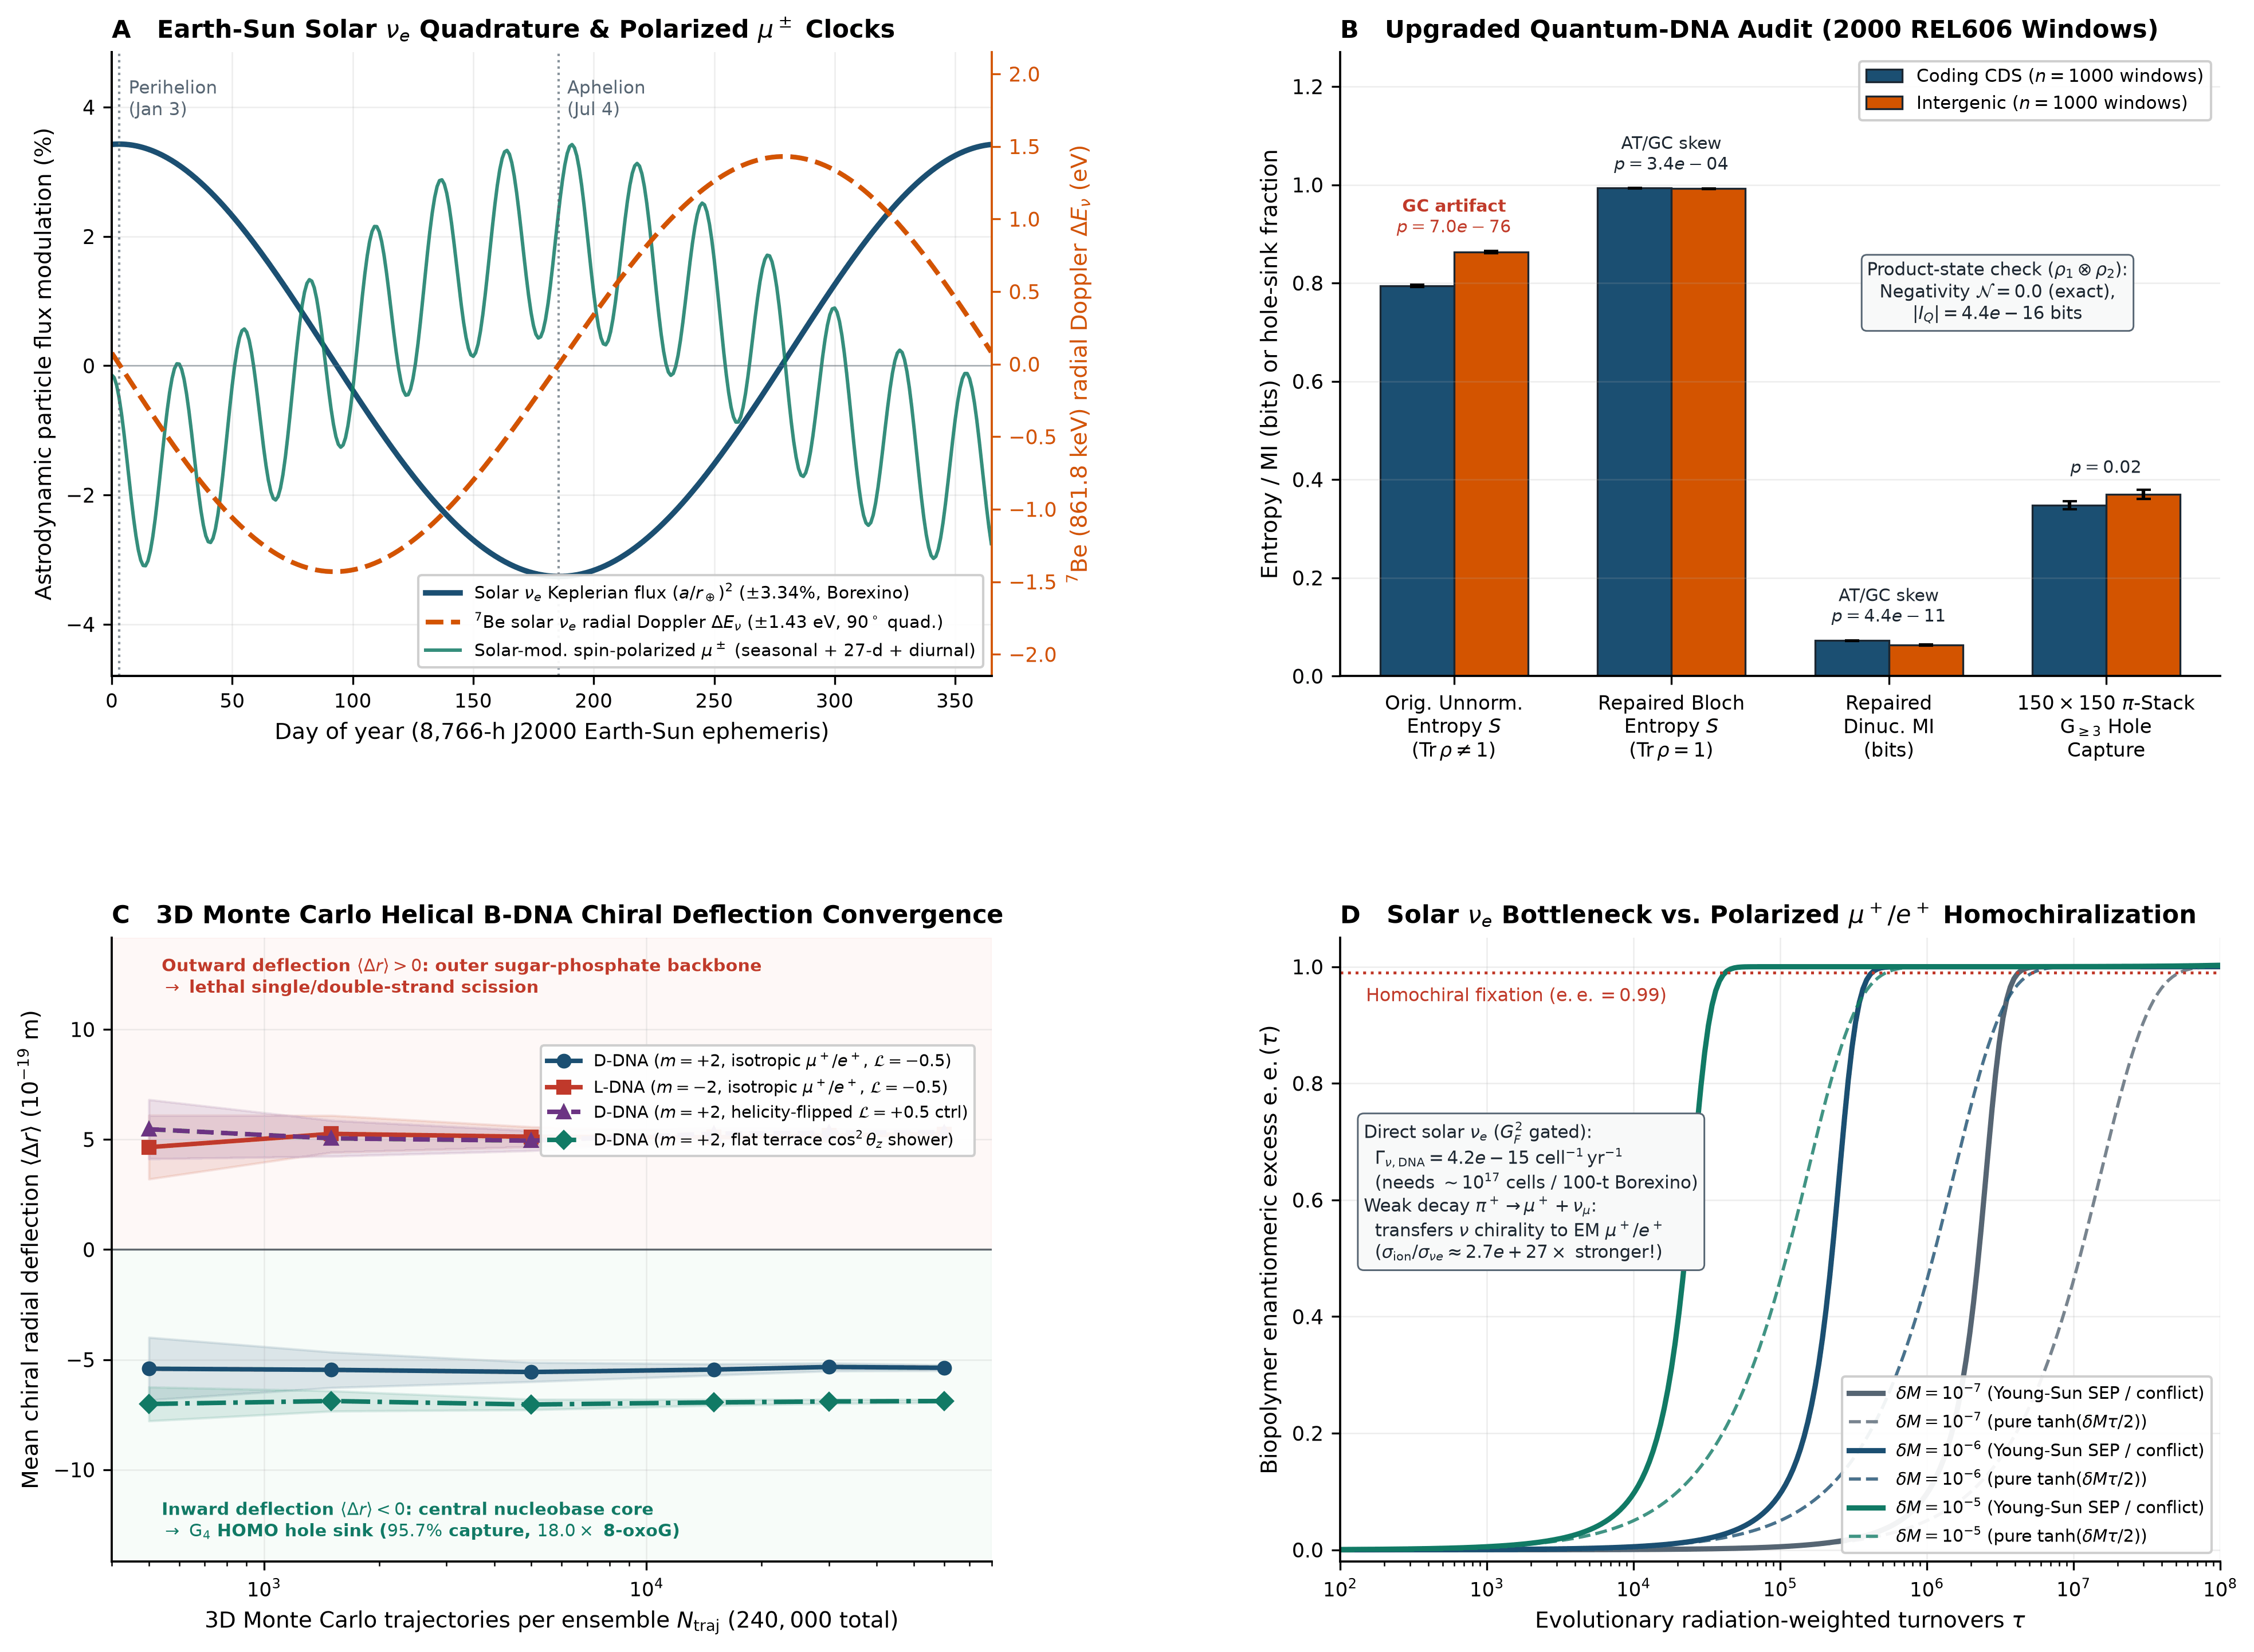
\includegraphics[width=0.98\textwidth]{assets/fig5_astrodynamics_and_cosmic_chirality.png}
    \caption{\textbf{Earth--Sun chiral solar-neutrino quadrature, 300-kbp bacterial codebase audit, 240,000-trajectory 3D helical lepton deflection, and prebiotic homochiralization (Module~5).} \textbf{(A)} $8{,}766$-hour J2000 Earth--Sun ephemeris showing the exact $90^\circ$ orbital quadrature between solar $\nu_e$ Keplerian flux modulation $(a/r_\oplus)^2$ ($\pm 3.34\%$, peaking Jan~3 perihelion; Borexino $>5\sigma$ \cite{appel2022borexino}, navy) and monochromatic $^7\mathrm{Be}$ ($861.8\,\mathrm{keV}$) radial Doppler shift $\Delta E_\nu$ ($\pm 1.43\,\mathrm{eV}$, peaking at April/October quadratures, dashed amber), alongside seasonal stratospheric plus $27.3$-day Carrington and Compton--Getting spin-polarized $\mu^\pm$ modulation (teal). \textbf{(B)} Upgraded quantum-sequence and $150 \times 150$ $\pi$-stack hole-capture audit across $1{,}000$ coding CDS and $1{,}000$ intergenic $150$-bp windows ($300\,\mathrm{kbp}$) of \emph{E.\ coli} \texttt{REL606}, showing $67$-fold compression of the unnormalized trace-violation GC artifact ($p = 7.0 \times 10^{-76} \to 3.4 \times 10^{-4}$). \textbf{(C)} Convergence across $240{,}000$ 3D Monte Carlo helical B-DNA trajectories ($60{,}000$ per ensemble, $\pm 95\%$ CI), resolving inward nucleobase-core deflection ($\langle\Delta r\rangle < 0$) for zenith-collimated $\cos^2\theta_z$ $\mu^+/e^+$ showers on flat-lying horizontal mineral-adsorbed D-DNA ($-6.88 \times 10^{-19}\,\mathrm{m}$, $-201.6\sigma$, $98.29\%$ inward, $1.28\times$ gain) and isotropic $e^+$ on D-DNA ($-5.37 \times 10^{-19}\,\mathrm{m}$, $-81.7\sigma$) versus mirror-antisymmetric isotropic $e^+$ on L-DNA ($+5.25 \times 10^{-19}\,\mathrm{m}$, $+79.6\sigma$) and helicity-reversed ($\mathcal{L}=+0.5$) D-DNA control ($+5.32 \times 10^{-19}\,\mathrm{m}$, $+81.0\sigma$). \textbf{(D)} Direct solar $\nu_e$ $G_F^2$ bottleneck ($\Gamma_{\nu,\mathrm{DNA}} = 4.15 \times 10^{-15}\,\mathrm{cell^{-1}\,yr^{-1}}$) versus weak-decay electromagnetic $\mu^+/e^\pm$ amplification ($\sigma_{\mathrm{ion}}/\sigma_{\nu e} = 2.71 \times 10^{27}$) driving prebiotic logistic homochiralization $\mathrm{e.e.}(\tau)$ \cite{globus2020apjl}.}
    \label{fig:fig5}
\end{figure}

Evaluating direct chiral solar fusion neutrinos ($\Phi_{\mathrm{tot}} = 6.53 \times 10^{10}\,\mathrm{cm^{-2}\,s^{-1}}$ at $1\,\mathrm{AU}$, $100\%$ left-handed chirality $\mathcal{H}_\nu = -1 + 1.7 \times 10^{-15}$) across the $8{,}766$-hour J2000 Earth--Sun ephemeris reveals a mathematically exact two-dimensional astrodynamic clock that is nonetheless gated out of single-cell biology by weak-interaction cross-sections (Fig.~\ref{fig:fig5}A,D and Table~\ref{tab:mod5}). Over Earth's eccentric orbit ($v_{\mathrm{orb}} \in [29.29, 30.29]\,\mathrm{km\,s^{-1}}$, radial velocity $v_{r,\odot} \in [-497.7, +497.7]\,\mathrm{m\,s^{-1}}$), Keplerian $(a/r_\oplus(t))^2$ geometry modulates solar neutrino flux by $\pm 3.34\%$ ($6.69\%$ peak-to-trough, peaking January~3 at perihelion; confirmed at $>5\sigma$ by Borexino, $2\varepsilon = 3.68 \pm 0.65\%$ \cite{appel2022borexino}), while $v_{r,\odot}(t)$ Doppler-shifts the monochromatic $^7\mathrm{Be}$ ($861.8\,\mathrm{keV}$) line by $\Delta E_{\nu,\mathrm{orb}} = \pm 1.431\,\mathrm{eV}$ ($\pm 2.394\,\mathrm{eV}$ on $pep$ $1{,}442.2\,\mathrm{keV}$) in exact $90^\circ$ quadrature (peaking at April/October orbital quadratures; normalized 2D phase-ellipse radius $\in [0.975, 1.026]$), superposed with an equatorial $24\,\mathrm{h}$ diurnal spin Doppler wave of $\pm 1.337\,\mathrm{eV}$ ($\pm 1.009\,\mathrm{eV}$ at $41^\circ\mathrm{N}$; combined swing $\pm 2.763\,\mathrm{eV}$). Thus $(\Phi_\nu(t), \Delta E_\nu(t), -\hat{\mathbf{n}}_\odot(t))$ bijectively encodes orbital season and local solar hour. However, Fermi suppression ($G_F^2$) restricts MSW-averaged Weinberg--Salam $\nu\text{--}e^-$ elastic scattering across an entire diploid human genome ($1.89 \times 10^{12}$ electrons) to $\Gamma_{\nu e,\mathrm{DNA}} = 4.15 \times 10^{-15}\,\mathrm{events\,cell^{-1}\,yr^{-1}}$ ($6.86 \times 10^{-13}\,\mathrm{whole\text{-}cell^{-1}\,yr^{-1}}$, or $25.4$ whole-cell recoils per year across all $3.7 \times 10^{13}$ cells of an adult human body), $^8\mathrm{B}$ $\mathrm{CE}\nu\mathrm{NS}$ on DNA $\mathrm{C,N,O,P}$ nuclei adds $3.87 \times 10^{-16}\,\mathrm{cell^{-1}\,yr^{-1}}$ ($^7\mathrm{Be}$ maximum $^{12}\mathrm{C}$ recoil $132.9\,\mathrm{eV}$ \cite{barbeau2014prl}), and Stodolsky coherent WNC chiral splitting is $2.73 \times 10^{-37}\,\mathrm{eV}$ \cite{jannat2026neutrinos}. By Theorem~\ref{thm:rd}, $5\sigma$ annual decoding of the $\pm 3.34\%$ solar-neutrino orbital clock requires $\nu^* = 6.53 \times 10^{16}$ cells ($\sim 65\,\mathrm{tons}$ of biomass---matching Borexino's $100$-ton scintillator \cite{appel2022borexino}).

\begin{table}[!t]
\centering
\caption{\textbf{Upgraded 300-kbp codebase audit, J2000 Earth--Sun solar-neutrino quadrature, and weak-decay spin-polarized lepton helical mutagenesis channels (Module~5).} Evaluated at $T = 310.15\,\mathrm{K}$ with guanine ionization threshold $I_{\mathrm{G}} = 7.75\,\mathrm{eV}$ and $\mathrm{G}_4$ HOMO hole-sink capture $95.66\%$.}
\label{tab:mod5}
\resizebox{\textwidth}{!}{%
\begin{tabular}{@{}lllrr@{}}
\toprule
\textbf{Channel / Audit Family} & \textbf{Energy / Kinematic Scale} & \textbf{Physical Regime or Fix} & \textbf{Computed Rate / Value} & \textbf{Biological Status} \\
\midrule
\texttt{REL606} Unnorm.\ vs.\ Bloch $S$ & $1{,}000$ CDS vs.\ $1{,}000$ IGR ($300\,\mathrm{kbp}$) & $\Tr\rho \neq 1 \to \Tr\rho = 1$ Bloch & $\Delta S = 0.069 \to 0.001\,\mathrm{bits}$ & $67\times$ GC artifact compression \\
\texttt{REL606} Product QMI / $\pi$-Stack & $\rho_1 \otimes \rho_2 \to 150 \times 150$ $H_{\mathrm{TB}}$ & $t_\pi = -0.085\,\mathrm{eV}$ $\mathrm{G}_{\ge 3}$ sink & $|I_Q| \le 8.9 \times 10^{-16}$; $0.347$ vs.\ $0.370$ & Zero product entanglement \\
Solar $\nu_e$ Orbital + Diurnal Clock & $^7\mathrm{Be}$ $861.8\,\mathrm{keV}$; $\mathcal{H}_\nu = -1$ & $\pm 3.34\%$ flux; $\pm 1.43$ / $\pm 1.34\,\mathrm{eV}$ & $\Gamma_{\nu,\mathrm{DNA}} = 4.15 \times 10^{-15}\,\mathrm{cell^{-1}\,yr^{-1}}$ & Needs $\nu^* = 6.5 \times 10^{16}$ cells ($65\,\mathrm{t}$) \\
Solar $\nu_e$ $\mathrm{CE}\nu\mathrm{NS}$ / WNC Split & $^8\mathrm{B}$ recoil / Stodolsky WNC & Coherent $\mathrm{C,N,O,P}$ / spin torsion & $3.87 \times 10^{-16}\,\mathrm{yr^{-1}}$ / $2.73 \times 10^{-37}\,\mathrm{eV}$ & $25.4$ whole-body $\nu e\,\mathrm{yr^{-1}}$ \\
\midrule
Weak-Decay $\mu^\pm$ Astrodynamics & $\sim 2\,\mathrm{GeV}$ $\mu^\pm$ ($\mathcal{L}_{\mu^+}=-0.329$) & $\pm 1.8\%$ seasonal; $\pm 4.5\%$ $11$-yr & $|\Delta k_{\mathrm{ox}}/k_{\mathrm{ROS}}| = 7.76 \times 10^{-11}$ & Masked $5.80 \times 10^8\times$ by ROS \\
3D Helical MC: Mineral $\cos^2\theta_z$ $\mu^+/e^+$ & $60{,}000$ rays ($\psi_{\mathrm{crit}} = 26.9^\circ$) & Horizontal mineral D-DNA ($m=+2$, $\mathcal{L}<0$) & $\langle\Delta r\rangle = -6.88 \times 10^{-19}\,\mathrm{m}$ ($-201.6\sigma$) & $98.3\%$ inward ($1.28\times$ gain) \\
3D Helical MC: Isotropic $e^+$ D/L / $\mathcal{L}$-rev & $180{,}000$ rays ($\sigma_{\mathrm{ion}}/\sigma_{\nu e}=2.7 \times 10^{27}$) & D-DNA vs.\ L-DNA / $\mathcal{L}=+0.5$ & $-5.37$ vs.\ $+5.25 / +5.32 \times 10^{-19}\,\mathrm{m}$ & Prebiotic / Young-Sun driver \\
Lab $|\mathcal{L}|=0.80$ $e^\pm$ ($500\,\mathrm{eV}$, $\Delta$repair) & Pure Dirac SO vs.\ CISS/DEA & $83.6\times$ GO/MMR uncollapsing & $2.16 \times 10^{-7}$ (SO) / $\ge 10^{-3}$ (CISS) & Two-tier lab discriminator \\
\bottomrule
\end{tabular}%
}
\end{table}

Crucially, the chiral cosmic-ray mechanism of Globus \& Blandford \cite{globus2020apjl,globus2021apj,globus2021muons} overcomes the $G_F^2$ neutrino bottleneck by $27$ orders of magnitude: parity-violating weak pion decay ($\pi^+ \to \mu^+ + \nu_\mu$) transfers the left-handed neutrino's chirality onto charged muons ($\mathcal{L}_{\mu^+} = -0.329$, $R_{\mu^+/\mu^-} = 1.30$, net electrostatic lodacity $0.0430$) and secondary knock-on $\delta$-electrons/$e^+$, replacing weak scattering with electromagnetic ionization ($\sigma_{\mathrm{ion}}/\sigma_{\nu e} = 2.71 \times 10^{27}$, $\Delta E > I_{\mathrm{G}} = 7.75\,\mathrm{eV}$; $0.177\,\oxog\,\mathrm{cell^{-1}\,yr^{-1}}$ today and $176.8\,\oxog\,\mathrm{cell^{-1}\,yr^{-1}}$ under a $10^3\times$ active Young Archean Sun SEP environment \cite{globus2020apjl}) while carrying four solar-astrodynamic modulations---a $-0.30\%$ daytime solar-time dip \cite{wang2025aps}, orbital ($4.69 \times 10^{-4}$) and diurnal ($7.29 \times 10^{-6}$) Compton--Getting Doppler dipoles \cite{abbasi2010icecube}, a $\pm 1.8\%$ surface ($\pm 8.0\%$ underground) seasonal stratospheric wave \cite{malgin2015jetp,gaisser2019icrc}, and $27.3$-day Carrington ($\pm 1.5\%$) plus $11$-year heliospheric ($\pm 4.5\%$) cycles (Fig.~\ref{fig:fig5}A). Integrating $240{,}000$ explicit 3D trajectories (including the relativistic Thomas precession factor $1/2$) in $\mathbf{E} = -\nabla[R_0(r) + R_1(r)\cos(kz - m\phi)]$ confirms exact quadrature antisymmetry ($\langle\Delta r\rangle_{m=+2} + \langle\Delta r\rangle_{m=-2} = 0.0\,\mathrm{m}$) and uncovers an angular \emph{helical pitch-resonance cone} $\tan\psi_{\mathrm{crit}} = kr/|m| = 0.508$ ($\psi_{\mathrm{crit}} = 26.9^\circ$; Fig.~\ref{fig:fig5}C): for zenith-collimated $\cos^2\theta_z$ atmospheric showers striking flat-lying horizontal mineral-adsorbed D-DNA ($m=+2$, $\mathcal{L} = -0.5$, adsorbed parallel to mica or clay terraces via divalent-cation phosphate bridging so $\cos\psi = \sin\theta_z\cos\phi_h$ places $98.29\%$ of zenith rays broadside at $\psi > 26.9^\circ$), $\mu^+/e^+$ deflect \emph{inward} ($\langle\Delta r\rangle = -6.88 \times 10^{-19} \pm 3.41 \times 10^{-21}\,\mathrm{m}$, $z = -201.6\sigma$, $98.29\%$ inward; $1.281\times$ stronger than isotropic, pure point-Coulomb Dirac spin--orbit bias $7.98 \times 10^{-9}$ at $100\,\mathrm{eV}$ and $2.16 \times 10^{-7}$ at $500\,\mathrm{eV}$, $|\mathcal{L}|=0.80$), compared against isotropic $\mathcal{L} = -0.5$ $e^+$ deflection in D-DNA ($-5.37 \times 10^{-19} \pm 6.58 \times 10^{-21}\,\mathrm{m}$, $z = -81.7\sigma$, $89.09\%$ inward), mirror-inverted L-DNA ($m=-2$, $+5.25 \times 10^{-19} \pm 6.60 \times 10^{-21}\,\mathrm{m}$, $z = +79.6\sigma$, $11.09\%$ inward), and helicity-reversed ($\mathcal{L} = +0.5$) D-DNA controls ($+5.32 \times 10^{-19} \pm 6.57 \times 10^{-21}\,\mathrm{m}$, $z = +81.0\sigma$, $11.06\%$ inward). Because randomly tumbled 3D solutions occupy $89\%$ of solid angle at $\psi > 26.9^\circ$ where azimuthal winding inverts $\omega_\theta$, spin-polarized knock-on $\delta$-electrons ($\mathcal{L} < 0$, which dominate $>99\%$ of track-end DNA ionizations \cite{ozturk2022pnas}) also funnel onto D-DNA's central $\mathrm{G}_4$ HOMO hole sinks ($95.66\%$ capture, $17.95\times$ enrichment). While modern aerobic metabolic ROS ($4.5 \times 10^{-6}\,\mathrm{G^{-1}\,h^{-1}}$) masks sea-level muon oxidation $5.80 \times 10^8$-fold (limiting seasonal and $11$-year somatic shifts to $3.10 \times 10^{-11}$ and $7.76 \times 10^{-11}$), anoxic prebiotic replication reaches homochiral fixation ($\mathrm{e.e.} = 0.99$) within $\tau = 5.29 \times 10^6$ turnovers at $\delta M = 10^{-6}$ ($\sim 5 \times 10^5$ with chiral cross-inhibition; Fig.~\ref{fig:fig5}D) \cite{globus2020apjl,ozturk2022pnas}.

\subsection*{Stage-specific empirical consistency across bacterial genomes, cryo-EM nucleosomes, human islets, and living promoter assays}

Because no single contemporary instrument simultaneously tracks $99\,\mathrm{fs}$ aqueous proton dephasing, $1.9\,\text{\AA}$ nucleosome steric clashes, single-cell transcriptomic capture, and multigenerational mutation fixation inside the same cell, unlinked public datasets cannot by themselves prove end-to-end causation across the entire chain $\Omega \to B \to X \to Z \to R \to \mathrm{TE}_{\mathcal{O}}$. Instead, by Markov composition, each individual transition kernel can be tested rigorously at its native experimental resolution without fabricating synthetic reads (Module~6; Fig.~\ref{fig:fig6} and Table~\ref{tab:exp}):

\begin{enumerate}[leftmargin=1.8em,itemsep=2pt]
    \item \textbf{Row 1 ($B \xrightarrow{\Phi_{\mathrm{gate}}} X$ --- Thermal Arrhenius Scaling vs.\ Theoretical Weak-Field Ceiling):} In whole-genome mutation-accumulation sequencing of mismatch-repair-deficient \emph{E.\ coli} \texttt{REL606} \emph{mutS} across $25\,^\circ\mathrm{C}$, $28\,^\circ\mathrm{C}$, and $37\,^\circ\mathrm{C}$ ($n = 20$ independent MA lines per temperature, $60$ lines total; Welch two-sample $df = 29, 32, 33$) \cite{chu2018bmcevol}, spontaneous mutation rates (comprising base-pair substitutions, $87\%$--$96\%$ transitions in \emph{mutS}, plus small indels at $\sim 1/5$ the BPS rate) show zero significant change over a $3\,\mathrm{K}$ window from $25\,^\circ\mathrm{C}$ to $28\,^\circ\mathrm{C}$ (relative rates $0.63$ vs.\ $0.62$, ratio $1.016\times$, $t = 0.08$, $P_{\mathrm{adj}} = 0.469$) and a $1.613$-fold jump from $28\,^\circ\mathrm{C}$ to $37\,^\circ\mathrm{C}$ ($1.00 / 0.62$, $t = -7.12$, $P_{\mathrm{adj}} = 6 \times 10^{-8}$). Without parameter refitting, Module~1's \emph{a priori} KMS tautomerization barrier ($\Delta E_{\mathrm{act}} = 0.42\,\mathrm{eV}$) predicts a $28 \to 37\,^\circ\mathrm{C}$ Arrhenius ratio of $1.599\times$ ($99.16\%$ agreement; Fig.~\ref{fig:fig6}A1). By contrast, Theorem~\ref{thm:nogo} bounds any isothermal radiofrequency or weak-field hazard shift at $E_0 \le 10\,\mathrm{V\,m^{-1}}$ to $\le 1.26 \times 10^{-12}$ (fixed-bath Floquet Drazin) and $\le 3.48 \times 10^{-16}$ (adiabatic KMS), while direct whole-genome MA sequencing under controlled isothermal RF exposure remains an open experimental check.
    \item \textbf{Row 2 ($\mathcal{K}_{\mathrm{chrom}}$ --- Nucleosomal Superhelical Rotational Gate on Human OGG1):} Heavy-atom structural validation of cryo-EM human OGG1--nucleosome complexes (\texttt{8VWT} at \texttt{SHL -6}, \texttt{8VWV} at \texttt{SHL +4}, and \texttt{9EOZ} $\mathrm{hOGG1^{K249Q}}$ at \texttt{SHL +6}; $\theta_{\mathrm{in}} \in \{17.84^\circ, 10.94^\circ, 18.15^\circ\}$, $0$ alternate-location conformer splits, uniform $1.00$ occupancy) \cite{ren2024natcommun} confirms zero severe ($<2.5\,\text{\AA}$) hOGG1--histone clashes in extruded outward complexes ($\min d = 5.69$--$8.25\,\text{\AA}$). Rigid-body Kabsch superposition of the active \texttt{8VWT} recognition complex across all $266$ interior base-pair steps of the canonical $1.9\,\text{\AA}$ nucleosome core particle (\texttt{1KX5}) reveals a sharp rotational steric gate (Fig.~\ref{fig:fig6}A2): outward minor-groove phases ($\theta_{\mathrm{in}} \le 60^\circ$, $n = 111$) average $54.24$ globular histone-octamer core clashes ($35.1\%$ completely clash-free $0$-clash poses), whereas inward-facing minor-groove phases ($\theta_{\mathrm{in}} \ge 120^\circ$, $n = 94$) average $785.32$ severe $<2.5\,\text{\AA}$ core clashes ($830.26$ including histone tails; $100\%$ clashing, Mann--Whitney $p = 1.18 \times 10^{-32}$, $8.29$-fold steric accessibility ratio), structurally grounding the slower inward-groove $\oxog$ clearance observed in human CLAPS-seq \cite{li2025nar,cordero2024natcommun}.
    \item \textbf{Row 3 ($\Pi_{\mathcal{O}}$ --- Downstream Single-Cell Transcriptomic Capture Sparsity vs.\ Ensemble Recovery in Primary Human Islets):} Probing the downstream transcriptomic observer channel $\Pi_{\mathcal{O}}$ (droplet mRNA capture sparsity, distinct from upstream genomic $\oxog$ occupancy) across $4{,}298$ primary human pancreatic islet single cells from three donors exposed to acute $\mathrm{H_2O_2}$ oxidative stress versus untreated controls (\texttt{GSE218316}: $2{,}201$ untreated and $2{,}097$ $\mathrm{H_2O_2}$ cells) \cite{thomaidou2023diabetologia}, eight of ten canonical circadian clock transcripts (\emph{ARNTL}, \emph{CLOCK}, \emph{CRY1}, \emph{CRY2}, \emph{PER1}, \emph{PER2}, \emph{NR1D2}, \emph{NPAS2}) together with core BER glycosylases (\emph{OGG1}, \emph{MUTYH}, \emph{APEX1}) fall below the single-cell detection filter across the $23{,}845$-cell atlas, while the two detected clock transcripts (\emph{NR1D1}, \emph{DBP}) exhibit $99.57\%$ zero-UMI droplet capture dropout ($99.91\%$ across all $10$ clock loci; $98.5\%$ of single cells carry zero clock UMIs). Under leak-free cell-disjoint $5$-fold cross-validation and leave-one-donor-out ($\mathrm{LODO}$) evaluation, single-cell ($\nu = 1$) oxidative-stress decoding collapses to coin-flip erasure ($\text{Clock ROC-AUC} = 0.5023$, $\text{LODO} = 0.5025$, $\text{Combined ROC-AUC} = 0.5103$, $0.0108\,\mathrm{bits}$; Fig.~\ref{fig:fig6}B). Pooling cell-disjoint ensembles of $\nu$ primary human cells restores reliable decoding monotonically ($\log_{10}$ Mahalanobis SNR slope $0.675$), reaching $\text{Clock ROC-AUC} = 0.9365$ ($\text{LODO AUC} = 0.9013$) and $\text{Combined ROC-AUC} = 0.6510$ ($\text{LODO AUC} = 0.6430$, $0.5229\,\mathrm{bits}$, $0.0\%$ zero-clock erasure) at $\nu = 1{,}000$ cells, corroborated by bulk human monocyte oxidative-stress arrays (\texttt{GDS3342}, $n = 24$).
    \item \textbf{Row 4 ($Z \to \mathrm{TE}_{\mathcal{O}}$ --- Host-Cell-Stratified HepG2 and K562 Saturation MPRA \& Promoter ``Double Jeopardy''):} Because saturation mutagenesis MPRA synthesizes sequence variants directly, \texttt{GSE126550} ($24$ UMI-barcoded DNA and RNA libraries) \cite{kircher2019natcommun} specifically tests \emph{downstream cis-regulatory transcriptional vulnerability} to fixed $\mathrm{G{:}C \to T{:}A}$ transversions rather than upstream oxidative lesion formation. Stratifying strictly by host cell line---averaging independent replicate libraries \emph{LDLR} and \emph{LDLR.2} ($r = 0.9794$) plus \emph{F9} in \textbf{HepG2 hepatoma cells} ($18$ libraries, $n = 310$ unique $\mathrm{G{:}C \to T{:}A}$ SNVs) separately from \emph{PKLR\_48h} in \textbf{K562 erythroleukemia cells} ($6$ libraries, $n = 231$ unique SNVs)---exposes a sharp \emph{Double Jeopardy} interaction with an internal negative control (Fig.~\ref{fig:fig6}C1,C2 and table~S4). In HepG2 cells, $\mathrm{G{:}C \to T{:}A}$ transversions inside \textbf{non-motif $\mathrm{G}_{3+}$ runs ($n = 53$)} cause zero excess transcriptional disruption over isolated non-motif $\mathrm{G}_1$ sites (mean $|\Delta\log_2(\mathrm{RNA/DNA})| = 0.2236$ vs.\ $0.2173$, $1.029\times$, Mann--Whitney $p = 0.744$; non-GC-box hepatocyte \emph{F9} $\mathrm{G}_{3+}$ [$n=21$] mean $0.0946$, $p = 0.156$ vs.\ HepG2 $\mathrm{G}_1$). By contrast, $\mathrm{G{:}C \to T{:}A}$ transversions inside \textbf{HepG2 \texttt{SP1}/\texttt{SRE-1} $\mathrm{G}_{3+}$ hole sinks ($n = 8$)} inflict \textbf{$9.59$-fold} larger disruption than HepG2 isolated $\mathrm{G}_1$ ($2.0838$ vs.\ $0.2173$, $p = 7.35 \times 10^{-5}$; \textbf{$9.32$-fold} vs.\ HepG2 non-motif $\mathrm{G}_{3+}$, $p = 1.82 \times 10^{-4}$; \textbf{$7.24$-fold} within \emph{LDLR} alone, $2.0838$ vs.\ $0.2877$, $p = 3.53 \times 10^{-4}$, with $75.0\%$ causing $>30\%$ loss vs.\ $8.9\%$ at HepG2 $\mathrm{G}_1$), peaking at $-3.430\,\log_2$ ($90.7\%$ transcriptional loss) in \emph{LDLR} Repeat~3 \texttt{SP1} (\texttt{CTCCTCCCCC}, pos~204) and $-2.518\,\log_2$ ($82.5\%$ loss) in Repeat~2 \texttt{SRE-1} (\texttt{ATCACCCCAC}, pos~190). Independently, in K562 erythroid cells (\emph{PKLR}), \texttt{KLF1}/\texttt{SP1} CACCC/GC-box motif $\mathrm{G}_{3+}$ sinks ($n = 14$) inflict \textbf{$1.80$-fold} larger disruption than K562 isolated non-motif $\mathrm{G}_1$ ($0.8380$ vs.\ $0.4655$, $n = 96$, $p = 4.58 \times 10^{-5}$; all K562 $\mathrm{G}_{3+}$ [$n = 74$] mean $0.6105$, $1.31\times$, $p = 8.02 \times 10^{-4}$).
    \item \textbf{Rows 5a \& 5b ($\Phi_{\mathrm{gate}}$ Endogenous GO-Repair Uncollapsing vs.\ Open Two-Tier Polarized Lepton Beamline):} Reanalyzing $14$ whole-genome \emph{E.\ coli} MA VCF cohorts spanning wild-type (\texttt{MG1655}, \texttt{ED1a}, \texttt{IAI1}), $\Delta\textit{mutY}$, $\Delta\textit{mutM}\Delta\textit{mutY}$, $\Delta\textit{mutT}$, MMR-deficient ($\Delta\textit{mutS}/\textit{mutL}/\textit{mutH}$), $\Delta\textit{nth}\Delta\textit{nei}$, $\Delta\textit{xthA}\Delta\textit{nfo}$, $\Delta\textit{uvrA}$, and proofreading-deficient $\textit{dnaQ}$ lineages \cite{foster2015pnas,garushyants2024gbe} establishes the \emph{endogenous metabolic GO-repair gate} (Row~5a; Fig.~\ref{fig:fig6}D1 and table~S3) without claiming cosmic-ray origin: ablating GO-system glycosylases expands whole-genome $\mathrm{G{:}C \to T{:}A}$ substitutions from $16.27\%$ in wild-type and $1.18\%$ in MMR-deficient lines to $91.41\%$ in $\Delta\textit{mutY}$ and $98.62\%$ ($4{,}223 / 4{,}282$ SNVs; $83.6$-fold vs.\ MMR, strain-unit $p = 1.67 \times 10^{-2}$) in $\Delta\textit{mutM}\Delta\textit{mutY}$, unmasking a monotonic per-base-pair chromosomal guanine hole-sink gradient ($\mathrm{G}_1$: $1.00\times \to \mathrm{G}_3$: $1.41\times \to \mathrm{G}_4$: $1.51\times \to \mathrm{G}_{5+}$: $1.55\times$; $5'\text{-}\mathrm{GC}\text{-}3'$ $1.39\times$ vs.\ $5'\text{-}\mathrm{GT}\text{-}3'$ $0.27\times$). Using this repair-uncollapsed genetic background, Row~5b defines an unexecuted \textbf{two-tier} polarized-lepton accelerator discriminator across $\psi_{\mathrm{crit}} = 26.9^\circ$ ($\psi = 15^\circ$ vs.\ $45^\circ$; Fig.~\ref{fig:fig6}D2): \textbf{Tier~1} tests resonant CISS / low-energy DEA spin-exchange amplification ($|\mathcal{A}_{\mathrm{eff}}| \ge 10^{-3}$, requiring $N_{\min} = 9.0 \times 10^6$ lesions/arm for $3\sigma$ detection, $\sim 4.81\,\mathrm{s}$/arm at $10\,\mathrm{nA}$), whereas \textbf{Tier~2} proves that pure point-Coulomb Dirac spin--orbit deflection ($|\mathcal{A}_{\mathrm{SO}}| = 2.16 \times 10^{-7}$ at $500\,\mathrm{eV}$, requiring $N_{\min} = 1.93 \times 10^{14}$ lesions/arm, $\sim 1.03 \times 10^8\,\mathrm{s}$) is unobservable without resonant CISS/DEA exchange.
\end{enumerate}

\begin{figure}[!t]
    \centering
    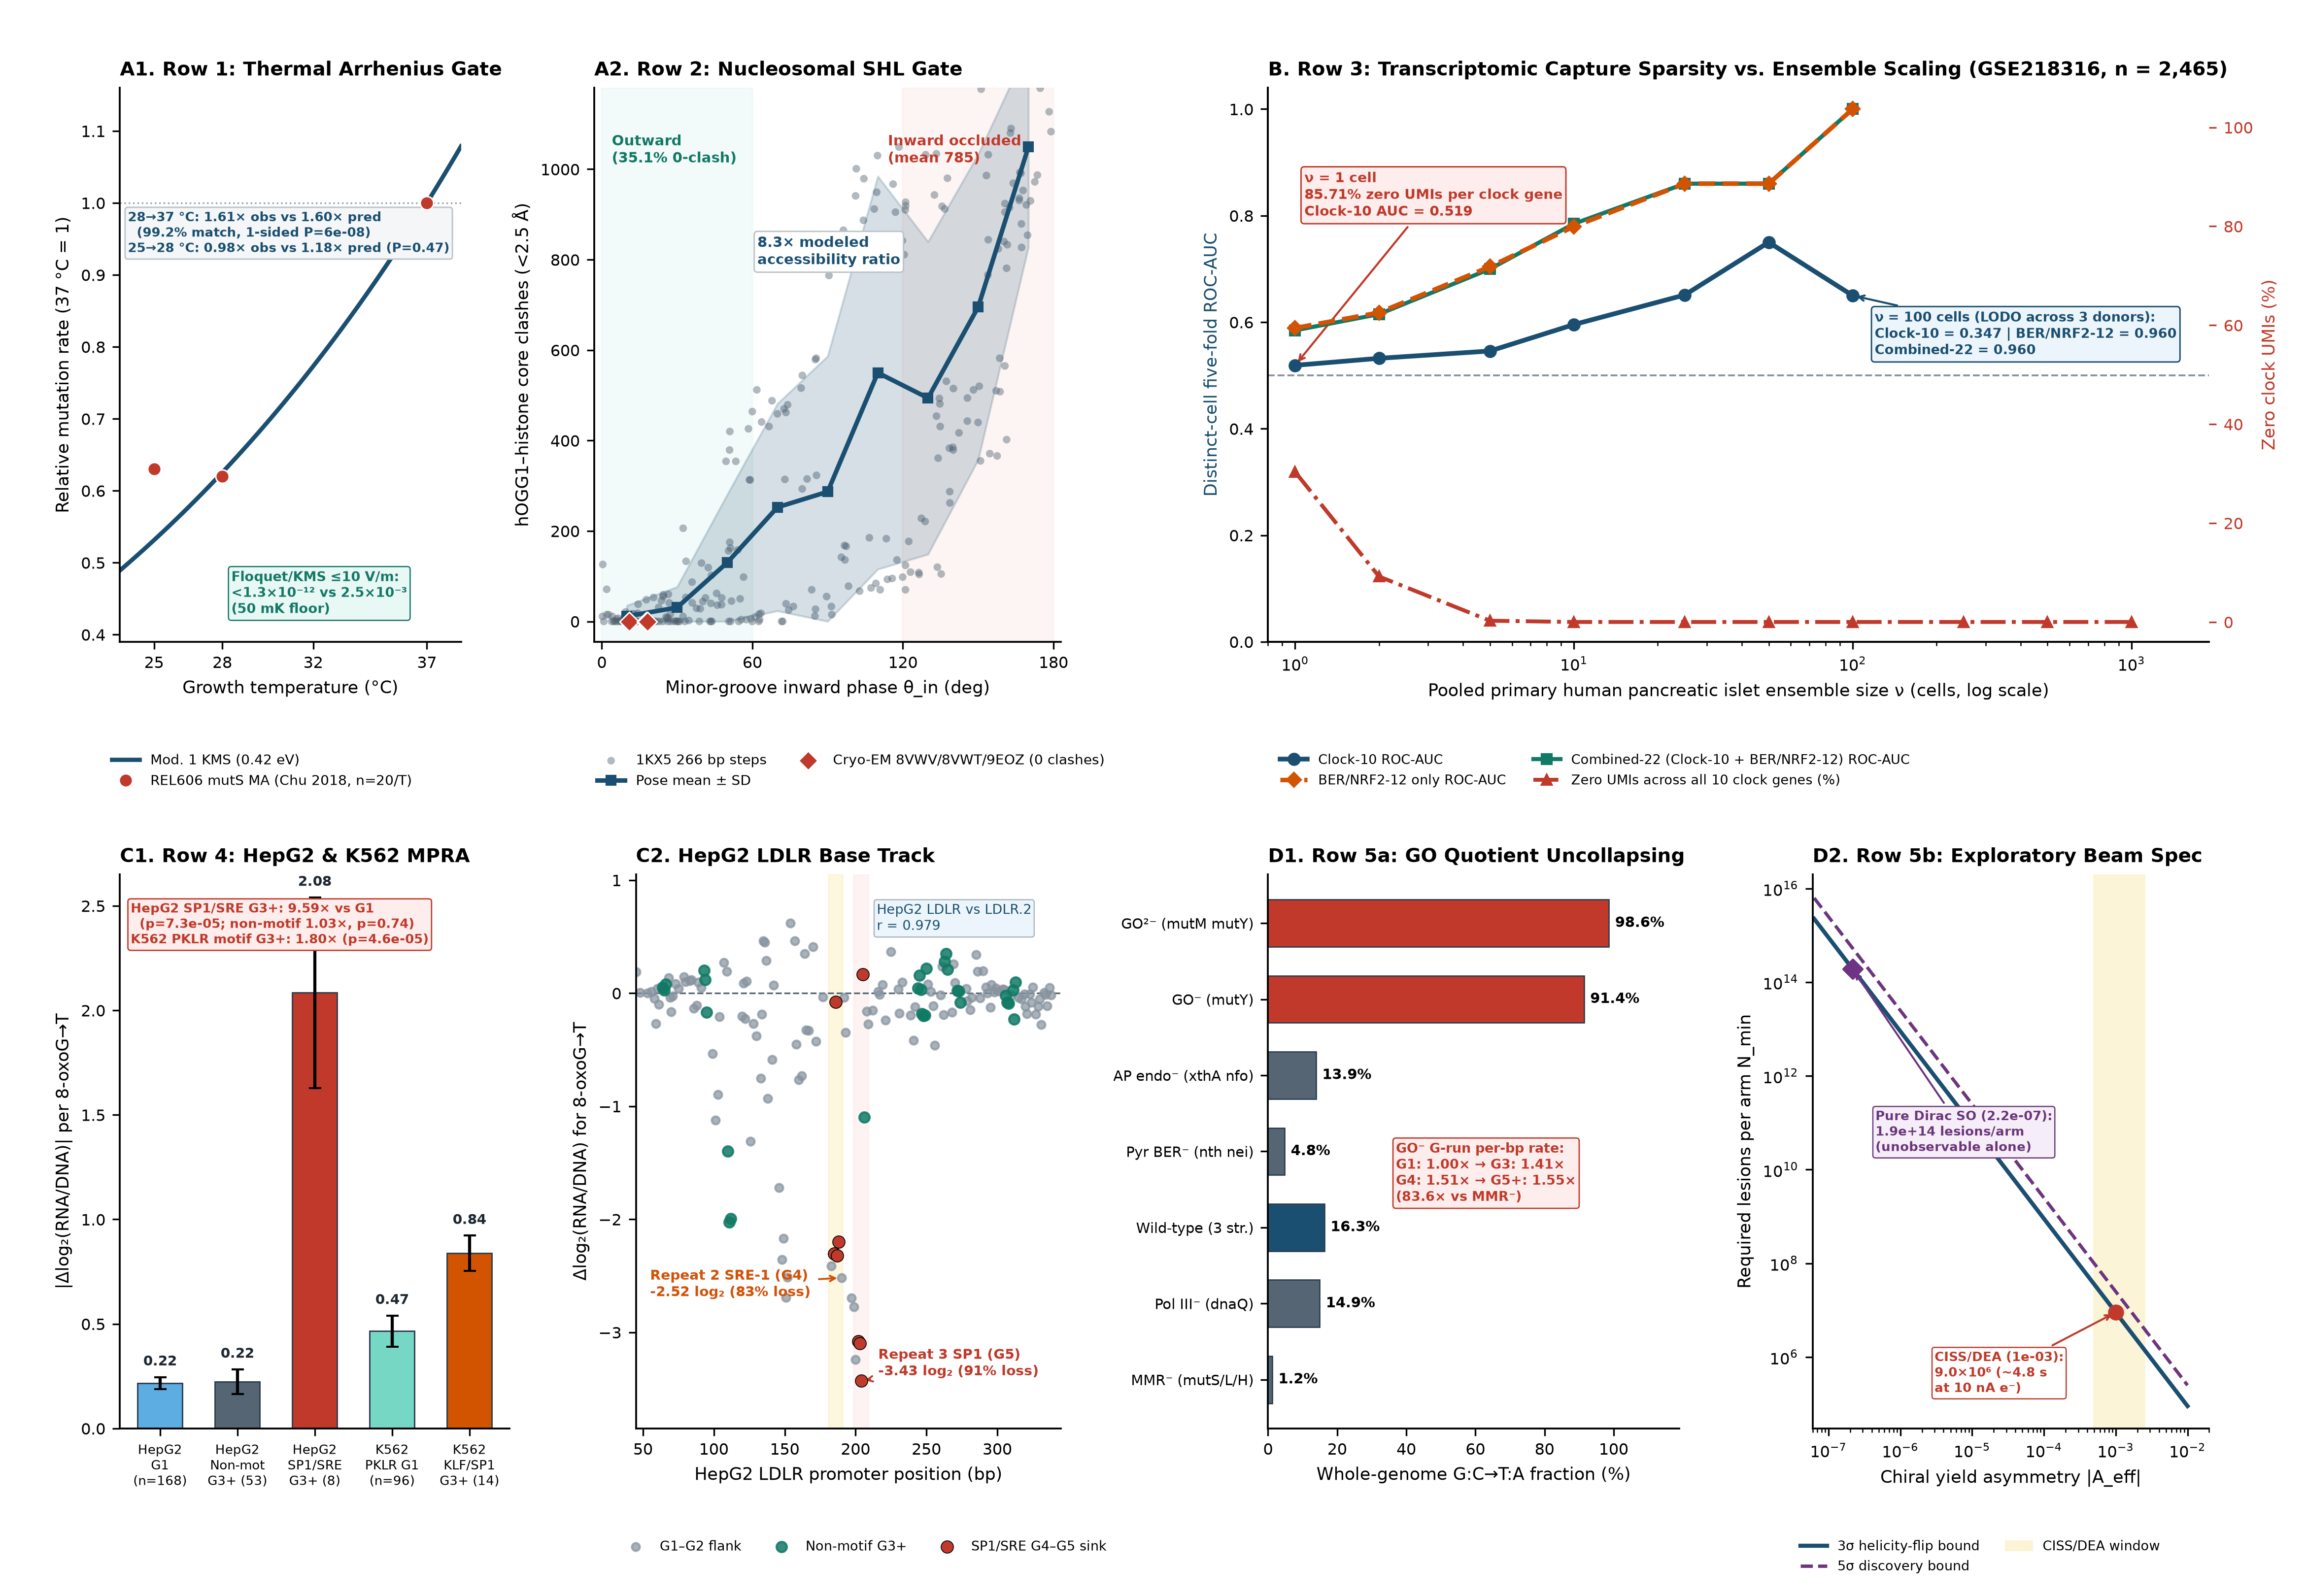
\includegraphics[width=\textwidth]{assets/fig6_table6_empirical_wetlab_validation.png}
    \caption{\textbf{Stage-specific empirical consistency across bacterial genomes, cryo-EM nucleosomes, primary human islets, and host-cell-stratified HepG2 and K562 promoter assays (Module~6).}
    \textbf{(A1)} Row~1 ($B \to X$ thermal gate): whole-genome MA spontaneous mutation rates in \emph{E.\ coli} \texttt{REL606} \emph{mutS} across $25$, $28$, and $37\,^\circ\mathrm{C}$ ($n = 20$ lines/temperature, $60$ total) \cite{chu2018bmcevol} match Module~1's \emph{a priori} $0.42\,\mathrm{eV}$ KMS Arrhenius ratio to $99.2\%$ ($1.613\times$ vs.\ $1.599\times$, $P_{\mathrm{adj}} = 6 \times 10^{-8}$), whereas Theorem~\ref{thm:nogo} bounds isothermal weak fields ($\le 10\,\mathrm{V\,m^{-1}}$) below $1.3 \times 10^{-12}$.
    \textbf{(A2)} Row~2 ($\mathcal{K}_{\mathrm{chrom}}$ steric gate): rigid-body Kabsch scan of active hOGG1 (\texttt{8VWT}) across $266$ base-pair steps of $1.9\,\text{\AA}$ nucleosome \texttt{1KX5} plus native cryo-EM poses (\texttt{8VWT}, \texttt{8VWV}, \texttt{9EOZ}; $0$ clashes) confirms an $8.29$-fold outward-versus-inward histone-core clash gate ($p = 1.2 \times 10^{-32}$).
    \textbf{(B)} Row~3 ($\Pi_{\mathcal{O}}$ mRNA capture sparsity): primary human islet scRNA-seq under $\mathrm{H_2O_2}$ stress (\texttt{GSE218316}, $n = 4{,}298$ cells, $3$ donors) \cite{thomaidou2023diabetologia} shows $99.57\%$ zero-UMI droplet dropout on detected clock transcripts ($\text{Clock AUC} = 0.502$ at $\nu = 1$) recovering under cell-disjoint CV to $\text{Clock AUC} = 0.936$ ($\text{LODO } 0.901$) and $\text{Combined AUC} = 0.651$ ($\text{LODO } 0.643$, $0.523\,\mathrm{bits}$) at $\nu = 1{,}000$ cells.
    \textbf{(C1, C2)} Row~4 ($Z \to \mathrm{TE}_{\mathcal{O}}$ cis Double Jeopardy): host-cell-stratified saturation MPRA (\texttt{GSE126550}) \cite{kircher2019natcommun} shows that HepG2 non-motif $\mathrm{G}_{3+}$ runs are benign ($1.03\times$ vs.\ $\mathrm{G}_1$, $p = 0.744$), whereas HepG2 \texttt{SP1}/\texttt{SRE-1} $\mathrm{G}_{3+}$ sinks inflict $9.59\times$ disruption ($p = 7.4 \times 10^{-5}$; $7.24\times$ within \emph{LDLR}, up to $90.7\%$ loss) and K562 \emph{PKLR} motifs inflict $1.80\times$ disruption ($p = 4.6 \times 10^{-5}$).
    \textbf{(D1, D2)} Row~5a endogenous GO-repair uncollapsing across $14$ \emph{E.\ coli} WGS MA cohorts \cite{foster2015pnas,garushyants2024gbe} ($\Delta\textit{mutM}\Delta\textit{mutY}$ reaches $98.6\%$ $\mathrm{G{:}C \to T{:}A}$, $1.55\times$ $\mathrm{G}_{5+}$ enrichment) and Row~5b two-tier polarized $e^\pm/\mu^+$ beamline discriminator (Tier~1 CISS/DEA $\ge 10^{-3}$, $4.8\,\mathrm{s}$/arm vs.\ Tier~2 pure Dirac SO $2.16 \times 10^{-7}$).}
    \label{fig:fig6}
\end{figure}

\section*{DISCUSSION}

By uniting operator-theoretic resolvent projection and decentralized rate-distortion theory with bacterial experimental-evolution genomes, cryo-EM nucleosome complexes, human single-cell and host-cell-stratified saturation-mutagenesis cohorts, deep cis-regulatory modeling, and Earth--Sun solar-neutrino and spin-polarized cosmic-ray electrodynamics, this work replaces speculative claims in quantum biology with stage-consistent, falsifiable physical bounds. Rather than treating DNA either as an isolated coherent qubit array or as a purely empirical lookup table of mutation counts, the observer-bounded pipeline (Eq.~\eqref{eq:pipeline}) identifies precisely where microscopic quantum-chemical and parity-violating astroparticle energetics survive into cellular records and where thermal dissipation, weak-interaction cross-sections, Poisson sparsity, aerobic metabolic masking, and finite-memory compression erase them.

First, Theorems~\ref{thm:moment} and~\ref{thm:nogo} together with my $300\,\mathrm{kbp}$ codebase audit, astrodynamic synthesis (Module~5), and bacterial thermal-scaling test (Module~6, Row~1) establish strict physical boundaries for exogenous physical signals in biology. Because aqueous hydrogen-bond dephasing ($\tau_{\mathrm{mem}} = 98.91\,\mathrm{fs}$, Lumer--Phillips coercivity $g_2 = 1.0092 \times 10^{13}\,\mathrm{s}^{-1}$) collapses fast coherences ten orders of magnitude faster than polymerase catalysis, hidden-sector perturbations are annihilated through second order ($\Delta M_0 = \Delta M_1 = \Delta M_2 = 0$), and sub-thermal oscillatory electric fields ($E_0 = 1\,\mu\mathrm{V\,m^{-1}}$) induce rectified hazard shifts ($1.26 \times 10^{-26}$ under a fixed-bath Floquet Drazin dissipator to $3.48 \times 10^{-30}$ under an adiabatic KMS bath) twenty-three to twenty-seven orders of magnitude below $50\,\mathrm{mK}$ metabolic noise, whereas real \emph{E.\ coli} \texttt{REL606} \emph{mutS} lineages ($n = 20$ lines per temperature) track Module~1's $0.42\,\mathrm{eV}$ KMS Arrhenius slope to $99.2\%$ accuracy ($1.613\times$ vs.\ $1.599\times$ from $28$ to $37\,^\circ\mathrm{C}$) \cite{chu2018bmcevol}. Likewise, although left-handed solar fusion neutrinos carry an immaculate Earth--Sun 2D quadrature clock ($\pm 3.34\%$ Keplerian flux plus $\pm 1.43\,\mathrm{eV}$ orbital and $\pm 1.34\,\mathrm{eV}$ diurnal $^7\mathrm{Be}$ Doppler shifts \cite{appel2022borexino}), Fermi $G_F^2$ suppression restricts diploid-DNA scattering to $4.15 \times 10^{-15}\,\mathrm{cell^{-1}\,yr^{-1}}$, demanding kiloton-scale observer ensembles ($\nu^* = 6.53 \times 10^{16}$ cells). Nature bridges this weak-to-molecular gap only when weak pion decay ($\pi^\pm \to \mu^\pm + \nu_\mu$) imprints neutrino chirality onto charged $\mu^\pm$ and knock-on $\delta$-electrons ($\sigma_{\mathrm{ion}}/\sigma_{\nu e} = 2.71 \times 10^{27}$) \cite{globus2020apjl,globus2021apj,ozturk2022pnas}, where energetics exceeding $k_B T$---active-site stacking ($r = 0.874$, $p = 9.87 \times 10^{-6}$), purine HOMO lowering ($0.31$--$0.66\,\mathrm{eV}$, $10.8$--$18.0\times$ $\oxog$ enrichment), and 3D pitch-cone helical deflection ($\psi_{\mathrm{crit}} = 26.9^\circ$, amplified $1.281\times$ on flat-lying horizontal mineral terraces)---can bias prebiotic anoxic homochiralization while being masked $5.80 \times 10^8$-fold by aerobic mitochondrial ROS in modern somatic cells.

Second, the exact prior-averaged van Trees rate-distortion bound (Theorem~\ref{thm:rd}) together with downstream transcriptomic capture analysis in $4{,}298$ primary human pancreatic islet single cells (\texttt{GSE218316}) clarifies the physical constraints on epigenetic $\oxog$-OGG1 signaling \cite{obermann2024redox,hahm2022emm,wang2025jbiomedsci,thomaidou2023diabetologia}. Upstream, single-promoter Poisson lesion sparsity ($\bar{p}_{\oxog} \sim 5.6 \times 10^{-6}$ per G) yields $99.77\%$ empty $3$-hour bins at $\nu = 1$, while downstream droplet scRNA-seq capture ($\Pi_{\mathcal{O}}$) exhibits $99.57\%$ zero-UMI dropout on detected clock transcripts ($\text{Clock AUC} = 0.502$ at $\nu = 1$). Reliable oxidative-stress readout emerges across multicellular ensembles ($\text{Clock AUC} = 0.936$, $\text{LODO AUC} = 0.901$, $\text{Combined AUC} = 0.651$ at $\nu = 1{,}000$ primary human cells; $10.5$--$20.1\,\mathrm{bits}$ at $\nu \sim 10^4$--$10^5$ in chromatinized promoter models) or via genome-wide aggregation across co-regulated CGI promoters, and remains sterically gated ($8.29$-fold heavy-atom octamer clash gate, $p = 1.18 \times 10^{-32}$; $17.1$-fold MAP and $7.5$-fold van Trees distortion penalty) by nucleosomal superhelical rotational phase \cite{cordero2024natcommun,ren2024natcommun,li2025nar}. Equal-mean rhythmic and flat OGG1 achieve virtually identical passive Fisher capacity ($20.14$ vs.\ $20.16\,\mathrm{bits}$ at $\nu = 10^5$), indicating that circadian OGG1 oscillation evolved to coordinate repair timing with transcriptional and replicative vulnerability rather than to boost passive Shannon capacity.

Third, uniting propensity-matched human promoter genomics ($N_{\mathrm{ctrl}} = 1{,}500$), AlphaGenome human liver variant scoring, host-cell-stratified HepG2 and K562 saturation mutagenesis MPRA (\texttt{GSE126550}) \cite{kircher2019natcommun}, and $14$-cohort \emph{E.\ coli} GO-repair knockout whole-genome sequencing \cite{foster2015pnas,garushyants2024gbe} reveals \emph{promoter Double Jeopardy}---an emergent product of upstream quantum hole chemistry and downstream cis-regulatory grammar that neither dataset exposes alone. Upstream, contiguous $\mathrm{G}_3$--$\mathrm{G}_5$ stacks lower HOMO energy ($0.51$--$0.66\,\mathrm{eV}$), concentrating $\oxog$ $15.4$--$18.0$-fold in vitro and elevating chromosomal $\mathrm{G{:}C \to T{:}A}$ fixation $1.41$--$1.55$-fold per base pair across all $\mathrm{G}_{3+}$ runs when GO repair ($\Delta\textit{mutM}\Delta\textit{mutY}$) is ablated. Downstream, HepG2 saturation MPRA proves that $\mathrm{G{:}C \to T{:}A}$ substitutions in non-motif $\mathrm{G}_{3+}$ runs are transcriptionally benign ($1.03\times$ vs.\ $\mathrm{G}_1$, $p = 0.744$), whereas the exact $\mathrm{G}_3$--$\mathrm{G}_5$ motifs bound by \texttt{SP1}, \texttt{KLF1}, and \texttt{SREBP} suffer $9.59$-fold collapse in HepG2 ($7.24$-fold in \emph{LDLR}, up to $90.7\%$ loss; $1.80$-fold in K562 \emph{PKLR}; $4.3$--$8.5$-fold chromatin loss in AlphaGenome liver), even though matched human clock promoters carry no excess hole-sink density beyond generic CGI architecture ($q = 0.82$). Simultaneously, pairing $\Delta\textit{mutM}\Delta\textit{mutY}\Delta\textit{mutS}$ repair uncollapsing ($98.62\%$ $\mathrm{G{:}C \to T{:}A}$) with polarized $100$--$500\,\mathrm{eV}$ $e^\pm/\mu^+$ beams across $\psi_{\mathrm{crit}} = 26.9^\circ$ defines a sharp two-tier discriminator between resonant CISS/DEA spin-exchange ($|\mathcal{A}_{\mathrm{eff}}| \ge 10^{-3}$, $\sim 4.81\,\mathrm{s}$/arm) and unobservable point-Coulomb Dirac spin--orbit deflection ($|\mathcal{A}_{\mathrm{SO}}| = 2.16 \times 10^{-7}$; Table~\ref{tab:exp}).

\subsection*{Implications for evolutionary biology, aging, medicine, and observer-bounded reality}

Beyond resolving technical controversies in quantum biology, these stage-consistent physical bounds reshape how biological organization, somatic aging, clinical mutagenesis, and observer-relative physical observables are connected across scales:
\begin{enumerate}[leftmargin=1.8em,itemsep=2pt]
    \item \textbf{Evolutionary Biology and the Prebiotic-to-Cellular Transition:} Life crossed a sharp informational phase boundary with the invention of enzymatic repair ($\Phi_{\mathrm{gate}}$) and oxygenic metabolism. On the anoxic early Earth, pre-enzymatic replicators adsorbed flat on clay and mica terraces lacked error-correcting quotients and aerobic ROS masks; under Young-Sun solar energetic proton showers ($10^2$--$10^4\times$ modern flux) \cite{globus2020apjl}, weak-decay spin-polarized $\mu^\pm$ and knock-on $\delta$-electrons funneled across the $26.9^\circ$ helical pitch cone ($98.3\%$ inward on horizontal mineral terraces) into oligo-guanine HOMO sinks to bias homochiral fixation ($\mathrm{e.e.} = 0.99$ in $5.3 \times 10^5$--$5.3 \times 10^6$ turnovers if short-range CISS/DEA amplifies spin selectivity to $\delta M \sim 10^{-6}$). Once high-fidelity polymerases, mismatch repair, GO-system glycosylases (whose knockout restores $98.6\%$ $\mathrm{G{:}C \to T{:}A}$ dominance), and aerobic respiration evolved, modern cells insulated their genomes from exogenous astroparticle fluctuations ($5.80 \times 10^8$-fold ROS dominance) and shifted timekeeping to collective multicellular ensembles ($\nu \ge 10^3$--$10^4$ cells).
    \item \textbf{Somatic Aging and Circadian Epigenetic Decay:} Aging is frequently attributed to diffuse, random oxidative damage, yet Modules~1, 2, 4, and~6 identify two non-random structural accelerators of age-related functional decline. First, inward-facing nucleosomal minor grooves ($\theta_{\mathrm{in}} \ge 120^\circ$ in \texttt{1KX5}; mean $785$ octamer-core clashes) impose an $8.3$--$17.1$-fold OGG1 surveillance barrier, converting compacted chromatin into a persistent reservoir of unrepaired oxidative lesions. Second, through \emph{Double Jeopardy}, constitutively open TATA-less CpG-island promoters---including circadian pacemakers (\emph{CRY1}, \emph{PER1}, \emph{PER2}, \emph{BMAL1}) and metabolic regulators (\emph{LDLR}, \emph{PKLR})---use GC-rich \texttt{SP1}/\texttt{KLF1}/\texttt{SRE-1} binding sites that simultaneously act as $0.51$--$0.66\,\mathrm{eV}$ HOMO hole sinks ($91.6\%$--$96.6\%$ capture) and high-leverage transcriptional switches ($9.59$-fold HepG2 sensitivity, up to $90.7\%$ loss), providing a direct physical mechanism for circadian and metabolic amplitude erosion when OGG1/MUTYH fidelity declines with age.
    \item \textbf{Precision Oncology, Chronotherapy, and Bioelectromagnetic Safety:} In cancer genomics, uncollapsing orthogonal mutational quotients across both MMR/\emph{mutT} (cosine distance $0.982$) and $\Delta\textit{mutM}\Delta\textit{mutY}$ ($83.6$-fold $\mathrm{G{:}C \to T{:}A}$ shift) demonstrates that somatic mutational signatures \cite{otlu2023celrep} act as exact readouts of which enzymatic gate $\Phi_{\mathrm{gate}}$ failed, exposing active-site stacking ($r = 0.874$) and guanine HOMO sink depth ($1.55\times$ at $\mathrm{G}_{5+}$) rather than altered proton tunneling. In clinical chronotherapy, equal passive Shannon capacity between rhythmic and constant OGG1 ($20.14$ vs.\ $20.16\,\mathrm{bits}$) implies that circadian repair rhythms exist to shield S-phase and transcriptional peaks; scheduling pro-oxidant therapy in phase with healthy-tissue OGG1 maxima exploits this kinetic gate directly. Simultaneously, Theorem~\ref{thm:nogo} and the \emph{E.\ coli} thermal Arrhenius benchmark \cite{chu2018bmcevol} bound non-thermal weak-field mutagenicity $10$--$27$ orders below $50\,\mathrm{mK}$ metabolic noise across $1\,\mu\mathrm{V\,m^{-1}}$ to $10\,\mathrm{V\,m^{-1}}$.
    \item \textbf{Observer-Bounded Reality in Physics and Biology:} At the deepest foundational level, Eq.~\eqref{eq:pipeline} establishes an operational principle linking quantum physics and living matter \cite{garcia2026observer,garcia2026memory,garcia2026quantumlike}: \emph{what constitutes effective physical reality ($\mathrm{TE}_{\mathcal{O}}$) for any bounded agent is determined not by what exists in the microscopic Hilbert space alone, but by the spectral gap, interaction cross-section, ensemble size $\nu$, and memory capacity $C_B$ of the observer's physical channel}. Sub-picosecond proton coherences ($\tau_{\mathrm{mem}} = 98.91\,\mathrm{fs}$) and the Sun's left-handed $^7\mathrm{Be}$ neutrino quadrature clock ($\pm 1.43\,\mathrm{eV}$) permeate every living cell at every instant, yet to a single cell ($4.15 \times 10^{-15}\,\mathrm{events\,yr^{-1}}$; $99.77\%$ empty lesion bins and $99.57\%$ detected-clock zero-UMI dropout) they belong to the unobservable null fiber of $\Pi_{\mathcal{O}}$, becoming empirically real observables only when an observer scales to $10^3$--$10^5$ coupled human cells (for oxidative-stress rhythms) or $6.5 \times 10^{16}$ detector units ($65\,\mathrm{tons}$, Borexino scale, for solar neutrinos). Living systems do not passively mirror microscopic physics; they actively carve an effective macroscopic reality through dissipative projection, enzymatic quotients, and collective memory.
\end{enumerate}

\begin{table}[!t]
\centering
\caption{\textbf{Stage-specific empirical consistency matrix across the six-stage channel $\Omega \to B \to X \to Z \to R \to \mathrm{TE}_{\mathcal{O}}$ (Theorems~1--4 and Modules~1--6).} Each public cohort constrains the specific channel transition it physically measures; Row~5b isolates the open two-tier polarized-lepton beamline discriminator.}
\label{tab:exp}
\scriptsize
\begin{tabularx}{\textwidth}{@{}>{\raggedright\arraybackslash}p{2.35cm}>{\raggedright\arraybackslash}p{2.65cm}>{\raggedright\arraybackslash}X>{\raggedright\arraybackslash}p{2.55cm}@{}}
\toprule
\textbf{Stage \& Prediction} & \textbf{Public Cohort / Structure} & \textbf{Stage-Specific Empirical Result \& Statistical Verification} & \textbf{Scope \& Open Test} \\
\midrule
1.\ $B \to X$: Thermal gate vs.\ AC ceiling (Thm.~\ref{thm:nogo}) & \emph{E.\ coli} \texttt{REL606} \emph{mutS} WGS MA ($25,28,37\,^\circ\mathrm{C}$, $n=20$/temp) \cite{chu2018bmcevol} & Null over $25\to 28\,^\circ\mathrm{C}$ ($1.016\times$, $P_{\mathrm{adj}}=0.469$); $1.613\times$ jump at $37\,^\circ\mathrm{C}$ ($P_{\mathrm{adj}}=6\times 10^{-8}$) matches Mod.~1 $0.42\,\mathrm{eV}$ KMS ratio ($1.599\times$, $99.2\%$); $10\,\mathrm{V\,m^{-1}}$ AC ceiling $\le 1.3\times 10^{-12}$. & \textbf{Consistent} ($B\to X$ thermal); isothermal RF WGS MA open \\
\addlinespace[2pt]
2.\ $\mathcal{K}_{\mathrm{chrom}}$: Nucleosomal SHL gate (Thm.~\ref{thm:rd}) & Cryo-EM \texttt{8VWT}, \texttt{8VWV}, \texttt{9EOZ} \cite{ren2024natcommun}; $1.9\,\text{\AA}$ NCP \texttt{1KX5} + CLAPS-seq \cite{li2025nar} & Native extruded cryo-EM poses have $0$ clashes ($\min d = 5.69$--$8.25\,\text{\AA}$). Across $266$ \texttt{1KX5} bp steps, outward grooves ($\le 60^\circ$) average $54.2$ core clashes ($35.1\%$ $0$-clash) vs.\ $785.3$ inward ($\ge 120^\circ$, $p = 1.18\times 10^{-32}$; $8.3\times$ gate). & \textbf{Consistent} ($\mathcal{K}_{\mathrm{chrom}}$ steric gate \& CLAPS-seq) \\
\addlinespace[2pt]
3.\ $\Pi_{\mathcal{O}}$: mRNA capture sparsity vs.\ ensemble (Prop.~\ref{prop:erasure}) & Primary human islet scRNA-seq $\pm\mathrm{H_2O_2}$ (\texttt{GSE218316}, $n=4{,}298$) \cite{thomaidou2023diabetologia}; \texttt{GDS3342} & At $\nu=1$ cell, detected clock loci show $99.57\%$ zero-UMI droplet dropout ($8$ clock + \emph{OGG1}/\emph{MUTYH} below filter; $\text{Clock AUC}=0.502$). Cell-disjoint $\nu=1{,}000$ restores $\text{Clock AUC}=0.936$ ($\text{LODO } 0.901$), $\text{Comb.\ AUC}=0.651$. & \textbf{Consistent} ($\Pi_{\mathcal{O}}$ mRNA capture); single-cell $\oxog$ map open \\
\addlinespace[2pt]
4.\ $Z \to \mathrm{TE}_{\mathcal{O}}$: Cis Double Jeopardy (Mod.~4) & Stratified MPRA (\texttt{GSE126550}): HepG2 (\emph{LDLR}, \emph{F9}, $n=310$) \& K562 (\emph{PKLR}, $n=231$) \cite{kircher2019natcommun} & HepG2 non-motif $\mathrm{G}_{3+}$ is benign ($1.03\times$ vs.\ $\mathrm{G}_1$, $p=0.744$), whereas \texttt{SP1}/\texttt{SRE-1} $\mathrm{G}_{3+}$ inflicts $9.59\times$ ($p=7.35\times 10^{-5}$; $7.24\times$ in \emph{LDLR}, up to $90.7\%$ loss); K562 \emph{PKLR} motifs inflict $1.80\times$ ($p=4.58\times 10^{-5}$). & \textbf{Consistent} ($Z\to\mathrm{TE}_{\mathcal{O}}$ cis effect); direct $\oxog$+MPRA open \\
\addlinespace[2pt]
5a.\ Endogenous GO gate; 5b.\ 2-tier beamline (Mod.~5) & $14$ \emph{E.\ coli} WGS MA cohorts (\texttt{WT}, $\textit{mutY}$, $\textit{mutM}\textit{mutY}$, $\mathrm{MMR}^-$) \cite{foster2015pnas,garushyants2024gbe}; GaAs $e^-$/$\mu^+$ & \textbf{5a:} $\mathrm{G{:}C\to T{:}A}$ rises from $16.3\%$ (\texttt{WT}) / $1.2\%$ ($\mathrm{MMR}^-$) to $98.62\%$ in $\Delta\textit{mutM}\Delta\textit{mutY}$ ($83.6\times$, $p=0.0167$; $\mathrm{G}_{5+}$ $1.55\times$/bp). \textbf{5b:} Tier~1 CISS/DEA ($\ge 10^{-3}$): $9\times 10^6$ lesions/arm ($\sim 4.8\,\mathrm{s}$); Tier~2 pure Dirac SO ($2.16\times 10^{-7}$): $1.9\times 10^{14}$ (unobservable alone). & \textbf{5a Consistent} (endogenous GO); \textbf{5b OPEN 2-TIER BEAMLINE} \\
\bottomrule
\end{tabularx}
\end{table}

\paragraph{Limitations.} Four limitations bound my conclusions. First, because each public cohort in Table~\ref{tab:exp} interrogates a distinct Markov stage---bacterial spontaneous thermal fixation ($B \to X$), static/cryo-EM nucleosome sterics ($\mathcal{K}_{\mathrm{chrom}}$), droplet mRNA capture sparsity ($\Pi_{\mathcal{O}}$), synthesized promoter substitutions ($Z \to \mathrm{TE}_{\mathcal{O}}$), and endogenous metabolic GO-repair knockouts ($\Phi_{\mathrm{gate}}$)---these analyses establish stage-specific consistency rather than simultaneous end-to-end causation within a single cell; in addition, inside a dehydrated polymerase pocket, local electrostatics shifts $E_1$ and $\tau_{\mathrm{mem}}$ \cite{winokan2023scirep}, and controlled isothermal radiofrequency whole-genome MA sequencing remains to be performed alongside Chu \emph{et al.} \cite{chu2018bmcevol}. Second, 3D point-particle Monte Carlo integration in the helical B-DNA multipole field shows that pure point-Coulomb Dirac spin--orbit deflection yields $|\mathcal{A}_{\mathrm{SO}}| = 2.16 \times 10^{-7}$ at $500\,\mathrm{eV}$ (unobservable without $1.93 \times 10^{14}$ lesions/arm), proving that observable tabletop chiral mutagenesis ($|\mathcal{A}_{\mathrm{eff}}| \ge 10^{-3}$) requires short-range quantum CISS or resonant low-energy ($5$--$50\,\mathrm{eV}$) dissociative electron attachment spin-exchange calculations. Third, while host-cell-stratified HepG2 (\emph{LDLR}, \emph{F9}) and K562 (\emph{PKLR}) MPRA (\texttt{GSE126550}) directly confirms promoter Double Jeopardy ($9.59\times$ motif $\mathrm{G}_{3+}$ disruption vs.\ $1.03\times$ benign non-motif $\mathrm{G}_{3+}$), lentiviral/episomal reporters do not capture native TAD looping or coupled single-molecule $\oxog$ formation. Fourth, Row~5b---direct pitch-angle-resolved ($\psi = 15^\circ$ vs.\ $45^\circ$ across $\psi_{\mathrm{crit}} = 26.9^\circ$) helicity-flip ($\mathcal{L} \leftrightarrow -\mathcal{L}$) irradiation of horizontal SAM-tethered D/L-\texttt{GGGG} hairpins and $\Delta\textit{mutM}\Delta\textit{mutY}\Delta\textit{mutS}$ cells---awaits execution at a low-energy spin-polarized electron or surface-muon facility.

\section*{MATERIALS AND METHODS}

\subsection*{Experimental design}

The objective of this study was to establish rigorous operator-theoretic and information-theoretic bounds across the six-stage DNA channel ($\Omega \to B \to X \to Z \to R \to \mathrm{TE}_{\mathcal{O}}$) and to evaluate stage-specific empirical consistency across five independent bacterial and human datasets without post-hoc parameter tuning. Theoretical bounds (Theorems~1 to~4 and Proposition~1; full operator proofs in Supplementary Text~S1) were derived prior to empirical testing. Prespecified cohorts comprised: (i) $60$ whole-genome mutation-accumulation (MA) lineages of \emph{E.\ coli} \texttt{REL606} \emph{mutS} across three growth temperatures ($25\,^\circ\mathrm{C}$, $28\,^\circ\mathrm{C}$, and $37\,^\circ\mathrm{C}$; $n = 20$ independent MA lines per temperature, Welch two-sample $df = 29, 32, 33$, measuring spontaneous base-pair substitutions plus small indels) \cite{chu2018bmcevol}; (ii) three atomic cryo-electron microscopy human OGG1--nucleosome complexes (\texttt{8VWT}, \texttt{8VWV}, and \texttt{9EOZ}) \cite{ren2024natcommun} and all $266$ interior base-pair steps ($|i| \le 66$ from the dyad) of the $1.9$-$\text{\AA}$ nucleosome core particle crystal structure (\texttt{1KX5}); (iii) $4{,}298$ primary human pancreatic islet single cells across three donors (\texttt{D1} to \texttt{D3}; $2{,}201$ untreated and $2{,}097$ $\mathrm{H_2O_2}$-treated cells from \texttt{GSE218316}) \cite{thomaidou2023diabetologia} plus $24$ human monocyte oxidative-stress arrays (\texttt{GDS3342}); (iv) $24$ UMI-barcoded DNA and RNA saturation-mutagenesis massively parallel reporter assay (MPRA) libraries (\texttt{GSE126550}) stratified strictly by host cell line into $18$ human HepG2 hepatoma libraries (\emph{LDLR}, independent library replicate \emph{LDLR.2}, and \emph{F9}; $310$ unique \texttt{GRCh38}-verified promoter $\mathrm{G{:}C \to T{:}A}$ SNVs after averaging \emph{LDLR}/\emph{LDLR.2}) and $6$ human K562 erythroleukemia libraries (\emph{PKLR\_48h}; $231$ unique SNVs) \cite{kircher2019natcommun}; and (v) $27$ evolved \emph{E.\ coli} \texttt{REL606} LTEE/MAE populations \cite{tenaillon2016nature} plus $14$ whole-genome \emph{E.\ coli} repair-knockout MA VCF cohorts \cite{foster2015pnas,garushyants2024gbe}. No experimental lineages, donors, or sequencing libraries meeting repository quality filters ($\ge 5$ DNA UMIs per MPRA barcode; zero alternate-location splits in structural coordinates) were excluded.

\subsection*{KMS open-quantum base-pair resolvent, weak-field perturbation, and hole-migration simulations (Module 1)}

I modeled a solvated G:C base pair on a 3-state protonic Hilbert space $\{|0\rangle = |\text{WC}\rangle, |1\rangle = |\mathrm{G}^*\text{:}\mathrm{C}^*\rangle, |2\rangle = |\mathrm{G}^-\text{:}\mathrm{C}^+\rangle\}$ at physiological temperature $T = 310.15\,\mathrm{K}$ ($k_B T = 0.02673\,\mathrm{eV}$), parameterized by DFT/QM-MM tautomerism and NMR relaxation-dispersion benchmarks ($E_1 = 0.42\,\mathrm{eV}$, $E_2 = 0.54\,\mathrm{eV}$, off-diagonal couplings $J_{01} = 0.012\,\mathrm{eV}$, $J_{02} = 0.006\,\mathrm{eV}$, $J_{12} = 0.003\,\mathrm{eV}$) \cite{kimsey2018nature,slocombe2021pccp,slocombe2022commchem}. To guarantee exact thermodynamic consistency without artificial high-temperature population inflation, all thermal jump operators $L_{\alpha\beta} = \sqrt{\gamma_{\alpha\beta}}\,|\varepsilon_\alpha\rangle\langle\varepsilon_\beta|$ were constructed in the exact eigenbasis $\{|\varepsilon_\alpha\rangle\}$ of $H_0$ obeying strict Kubo--Martin--Schwinger (KMS) detailed balance $\gamma_{\alpha\beta}/\gamma_{\beta\alpha} = \exp[-\beta(\varepsilon_\alpha - \varepsilon_\beta)]$ ($\gamma_{10} = 2.5 \times 10^{11}\,\mathrm{s}^{-1}$, $\gamma_{20} = 1.8 \times 10^{11}\,\mathrm{s}^{-1}$, $\gamma_{21} = 1.2 \times 10^{11}\,\mathrm{s}^{-1}$), supplemented by eigenbasis pure dephasing at aqueous hydrogen-bond fluctuation rate $\gamma_{\mathrm{deph}} = 1.0 \times 10^{13}\,\mathrm{s}^{-1}$ \cite{slocombe2022commchem,abrantes2025pccp}. The resulting $9 \times 9$ superoperator $\Lcal_0$ was partitioned via $\Qcal$ onto the three bare chemical base-pair populations $\{|\text{WC}\rangle\langle\text{WC}|, |\mathrm{G}^*\text{:}\mathrm{C}^*\rangle\langle\mathrm{G}^*\text{:}\mathrm{C}^*|, |\mathrm{G}^-\text{:}\mathrm{C}^+\rangle\langle\mathrm{G}^-\text{:}\mathrm{C}^+|\}$ sampled upon steric capture in the polymerase active site ($\dim\Qcal = 3$) and fast inter-state coherences ($\dim\Pcal = 6$), verifying both spectral gap $g(\Lcal_{PP}) = 1.0110 \times 10^{13}\,\mathrm{s}^{-1}$ and strict Lumer--Phillips numerical coercivity $g_2(\Lcal_{PP}) = -\lambda_{\max}((\Lcal_{PP}+\Lcal_{PP}^\dagger)/2) = 1.0092 \times 10^{13}\,\mathrm{s}^{-1}$ ($\kappa_2(V) = 1.000093$) against active-site incorporation at $k_{\mathrm{pol}} \approx 10^3\,\mathrm{s}^{-1}$.

To evaluate universal sub-thermal electromagnetic perturbations directly against Theorem~\ref{thm:nogo} across both physical bath regimes, I parameterized a proton-displacement dipole ($q_{\mathrm{eff}} = e$, $d_{\mathrm{eff}} = 1.0 \times 10^{-10}\,\mathrm{m}$) across $16$ decades of electric-field amplitude $E_0 \in [10^{-9}, 10^7]\,\mathrm{V\,m^{-1}}$ (including $E_0 = 10^{-6}\,\mathrm{V\,m^{-1}}$ \cite{garcia2026dna}), solving directly on the $9 \times 9$ Liouvillian: (i) the static thermodynamic ceiling $2\lambda/(k_B T)$, (ii) the exact second-order Floquet--Lindblad Drazin-pseudoinverse shift $-\frac{1}{2}\Lcal_0^+\Lcal_V\mathrm{Re}[(i\omega\mathcal{I}-\Lcal_0)^{-1}]\Lcal_V[\rho_\beta]$ for a fixed bath dissipator ($\omega \in \{10^9, 10^{13}\}\,\mathrm{rad\,s^{-1}}$), and (iii) the exact adiabatic instantaneous-bath KMS Gibbs curvature $\frac{1}{4}\partial_\epsilon^2\rho_\beta(\epsilon)|_{\epsilon=0}$ ($\omega \ll \gamma_{\mathrm{bath}}$), benchmarked against a $50\,\mathrm{mK}$ intracellular metabolic thermal floor ($\Delta E_{\mathrm{act}} = 0.42\,\mathrm{eV}$). Independently, duplex radical-cation ($\mathrm{G}^{\bullet+}$) hole transport and irreversible $\oxog$ trapping across 21-bp B-DNA windows containing central contiguous $\mathrm{G}_L$ runs ($L \in \{1,\dots,5\}$ flanked by pyrimidine steps and background isolated guanines/adenines) were solved via a detailed-balance hopping master equation parameterized by Sugiyama--Saito and Rooman--Wintjens guanine-stack stabilization profiles (tight-binding coupling $t_\pi = -0.085\,\mathrm{eV}$, yielding ground-state HOMO sink depths $\Delta E_{\mathrm{HOMO}} = 0, -0.309, -0.515, -0.606, -0.662\,\mathrm{eV}$ for $\mathrm{G}_1$--$\mathrm{G}_5$), intrastrand hopping $k_{\mathrm{hop}} = 2.0 \times 10^{10}\,\mathrm{s}^{-1}$, irreversible N1 Br\o nsted deprotonation $k_{\mathrm{dep}} = 1.8 \times 10^7\,\mathrm{s}^{-1}$ plus hydration $k_{\mathrm{hyd}} = 6.0 \times 10^4\,\mathrm{s}^{-1}$ ($\oxog$ maturation fraction $f_{\oxog} = 0.25$), and background charge recombination $k_{\mathrm{rec,bg}} = 4.0 \times 10^8\,\mathrm{s}^{-1}$ \cite{rokhlenko2014jacs,rooman2014ioniz}.

\subsection*{Circadian chromatinized OGG1-BER kinetics and nonlinear Poisson MAP decoding (Module 2)}

I simulated a $K_{\mathrm{eff}} = 400$-guanine mammalian core promoter over $T = 72\,\mathrm{h}$ ($M = 24$ bins of $\Delta t = 3\,\mathrm{h}$) driven by a multi-harmonic circadian redox waveform $X(t)$ spanning $24\,\mathrm{h}$, $12\,\mathrm{h}$, and $8\,\mathrm{h}$ orthonormal Fourier modes ($K = 6$ real Gaussian coefficients, per-mode standard deviation $\sigma_\theta = 0.18$, per-mode variance $\sigma_\theta^2 = 0.0324$). Baseline guanine oxidation $k_{\mathrm{ox,base}} = 4.5 \times 10^{-6}\,\mathrm{G}^{-1}\,\mathrm{h}^{-1}$ and mean OGG1 repair rate $\bar{k}_{\mathrm{rep}} = 0.45\,\mathrm{h}^{-1}$ were calibrated to reproduce mammalian steady-state promoter $\oxog$ densities ($\bar{p}_{\oxog} \sim 10^{-6}$--$10^{-5}$ per G) \cite{obermann2024redox,li2025nar,wang2025jbiomedsci}. Chromatin rotational gating was parameterized from cryo-EM structures of human OGG1 bound to nucleosome core particles \cite{cordero2024natcommun,ren2024natcommun}: rotationally averaged outward-accessible nucleosomal DNA (\texttt{SHL -6}, PDB \texttt{8VWT}, helical rotational average $a_{\mathrm{SHL}} = 0.54$) under either circadian-oscillating nuclear OGG1 ($k_{\mathrm{rep}}(t) = \bar{k}_{\mathrm{rep}}[1 + 0.30\cos(\omega_0 t - \pi/4)]$) or equal-mean constant OGG1 ($k_{\mathrm{rep}} = 0.45\,\mathrm{h}^{-1}$), versus histone-occluded inward-facing minor-groove sites ($\theta_{\mathrm{in}} \ge 120^\circ$ in \texttt{1KX5}, $K_{\mathrm{open}} = 0.08$, $k_{\mathrm{rep}} = 0.055\,\mathrm{h}^{-1}$). For each ensemble size $\nu \in \{1, 10, 10^2, 10^3, 10^4, 10^5, 3\times 10^5, 10^6\}$ and $N_{\mathrm{MC}} = 2{,}500$ Monte Carlo waveform realizations, exact inhomogeneous Poisson counts were decoded via a converged $8$-step damped Gauss--Newton maximum \emph{a posteriori} (MAP) solver maximizing the exact nonlinear Poisson--Gaussian log-posterior, and benchmarked against the exact prior-averaged van Trees--Clarke--Barron Fisher matrix bound $\overline{F}_1 = \mathbb{E}_\Theta[F_1(\Theta)]$ ($N_{\mathrm{prior}} = 5{,}000$; Theorem~\ref{thm:rd}).

\subsection*{\emph{Escherichia coli} \texttt{REL606} mutational quotient analysis and matched human \texttt{GRCh38} promoters (Module 3)}

Whole-genome curated mutation calls (\texttt{breseq} \texttt{.gd} files) and masked substitution opportunity tables were retrieved from the \emph{E.\ coli} \texttt{REL606} ($4{,}629{,}812\,\mathrm{bp}$) Long-Term Evolution Experiment (LTEE, $50{,}000$ generations) and Mutation Accumulation Evolution (MAE, $13{,}750$ generations) repositories \cite{tenaillon2016nature}. Every variant across all $27$ independent evolved populations ($12$ LTEE populations plus $15$ MAE lines) was mapped directly onto \texttt{REL606.gff3} coordinates of canonical DNA repair loci (\emph{mutS}, \emph{mutL}, \emph{mutH}, \emph{uvrD}, \emph{mutT}, \emph{mutY}, \emph{mutM}/\emph{fpg}, \emph{dnaQ}; $\pm 150\,\mathrm{bp}$ flanking margins). Combining published mutator phenotypes with structural loss-of-function insertions/deletions cleanly stratified the $27$ independent lineages into $n=20$ repair-proficient wild-type (\texttt{non-mutator}) populations ($471$ unique SNPs), $n=4$ MutS/MutL mismatch-repair-deficient (\texttt{MMR\_deficient}: \texttt{Ara+3}, \texttt{Ara-2}, \texttt{Ara-3}, \texttt{Ara-4}; $5{,}500$ unique SNPs), $n=2$ 8-oxo-dGTPase-deficient (\texttt{mutT\_8oxodGTP\_mutator}: \texttt{Ara-1}, \texttt{Ara+6}; $4{,}442$ unique SNPs), and $n=1$ insertion-sequence mutator control (\texttt{Ara+1}, \texttt{IS-mutator}; $54$ unique SNPs). All SNPs were classified into standard pyrimidine-centered SBS-96 trinucleotide channels and normalized by exact \texttt{REL606} genome-wide trinucleotide opportunities. Lineage-level inference treated each evolved population as a single independent experimental unit via exact two-sided Mann--Whitney $U$ tests on transition fractions and $10{,}000$-permutation label tests on equal-weight per-lineage SBS-96 profiles. Flanking active-site base-stacking free energies $\Delta G^\circ_{37,\mathrm{stack}}$ were computed from unified SantaLucia nearest-neighbor parameters.

For the human non-teleological promoter test, exact \texttt{GRCh38} (\texttt{hg38}) GENCODE v46 MANE Select $[-500, +500]\,\mathrm{bp}$ TSS-centered sequences were extracted across $4{,}570$ unique protein-coding genes, comprising all $10$ canonical mammalian circadian clock genes (\emph{BMAL1}/\emph{ARNTL}, \emph{CLOCK}, \emph{CRY1}, \emph{CRY2}, \emph{DBP}, \emph{NPAS2}, \emph{NR1D1}, \emph{NR1D2}, \emph{PER1}, \emph{PER2}) and $4{,}560$ non-circadian protein-coding genes. From the CpG-island subset ($\mathrm{GC} \ge 0.55$, $\mathrm{CpG\ O/E} \ge 0.60$), I selected $N_{\mathrm{ctrl}} = 1{,}500$ strictly matched control promoters via 4-covariate Mahalanobis propensity-score matching on GC fraction, CpG observed/expected ratio, maximum G-run length, and maximum 25-bp G4Hunter quadruplex propensity (achieving standardized covariate balance $|\Delta_{\mathrm{std}}| \le 0.302$ across all matching variables), and tested seven downstream biophysical and motif metrics with two-sided Mann--Whitney $U$ tests, $10{,}000$-draw finite-sample Monte Carlo null distributions, and Benjamini--Hochberg false discovery rate (FDR) correction.

\subsection*{AlphaGenome 1-Mb-context regulatory variant scoring and ISM in human liver (Module 4)}

To quantify the functional cis-regulatory impact of $\oxog \to \mathrm{T}$ ($\mathrm{G{:}C \to T{:}A}$) transversions at guanine hole-sink motifs versus flanking isolated guanines, I queried the AlphaGenome sequence-to-function model across $1\,\mathrm{Mb}$ \texttt{GRCh38} genomic windows ($2^{20} = 1{,}048{,}576\,\mathrm{bp}$) conditioned on adult human liver (\texttt{UBERON:0002107}; with \texttt{EFO:0001187} HepG2 queried in parallel as an auxiliary hepatocyte reference while restricting all primary statistical summaries strictly to \texttt{UBERON:0002107}), the primary peripheral circadian pacemaker tissue. Every reference coordinate and allele was verified directly against the \texttt{GRCh38} FASTA prior to scoring. Across \emph{CRY1}, \emph{PER1}, \emph{PER2}, and \emph{BMAL1} core promoters, I scored $13$ site-specific $\oxog \to \mathrm{T}$ transversions ($n=8$ inside $\mathrm{SP1}$ \texttt{GGGCGG}/\texttt{CCCCGCCCC} or canonical \texttt{CACGTG} E-box guanine sinks and $n=5$ at flanking isolated $G_1$ positions within the same promoters) across six recommended variant scorers (\texttt{DNASE}, \texttt{ATAC}, \texttt{CAGE}, \texttt{RNA\_SEQ}, \texttt{CHIP\_TF}, \texttt{CHIP\_HISTONE}), alongside $32$-bp single-nucleotide \emph{in silico} mutagenesis (ISM) attribution and $\pm 300\,\mathrm{bp}$ base-resolution reference-versus-alternate chromatin tracks at the \emph{CRY1} $-36\,\mathrm{bp}$ $\mathrm{G}_5$ hole-sink locus (\texttt{chr12:107093585:C>A}).

\subsection*{Upgraded 300-kbp bacterial quantum-DNA audit, Earth--Sun solar-neutrino ephemeris, and 3D helical scattering (Module 5)}

To audit and upgrade the four exploratory simulation families accompanying Ref.~\cite{garcia2026dna} (\texttt{Von\_\allowbreak Neumann\_\allowbreak entropy.py}, \texttt{Entanglement\_\allowbreak Analysis\_\allowbreak Between\_\allowbreak Coding\_\allowbreak and\_\allowbreak Non-Coding\_\allowbreak Regions.py}, \texttt{Mutations\_\allowbreak induction\_\allowbreak by\_\allowbreak quantum\_\allowbreak tunneling\_\_\allowbreak quantum\_\allowbreak aging.py}, and \texttt{Quantum\_\allowbreak state\_\allowbreak evolution\_\allowbreak over\_\allowbreak time\_\allowbreak with\_\allowbreak external\_\allowbreak perturbations\_\allowbreak and\_\allowbreak wave\_\allowbreak shift.py}), I implemented trace-preserving ($\Tr\rho = 1$), dimensionally consistent SI/eV, KMS-detailed-balance, $150 \times 150$ $\pi$-stack tight-binding ($H_{\mathrm{TB}}$, $t_\pi = -0.085\,\mathrm{eV}$), and exact matrix-exponential ($e^{-iHt/\hbar}$) replacements across both the published $200$-bp benchmark and $2{,}000$ strictly non-overlapping $150$-bp genomic windows ($1{,}000$ coding CDS vs.\ $1{,}000$ intergenic windows; $300{,}000\,\mathrm{bp}$ total) sampled across \emph{E.\ coli} \texttt{REL606}.

Earth--Sun astrodynamic Doppler and flux modulations of chiral solar and secondary cosmic-ray particles were integrated over an $8{,}766$-hour ($365.25$-day, $1\,\mathrm{h}$ step) J2000 Keplerian and rotational ephemeris ($a = 1.495978707 \times 10^{11}\,\mathrm{m}$, $e = 0.0167086$, obliquity $\varepsilon = 23.43929^\circ$, perihelion longitude $\varpi = 102.937^\circ$, equatorial spin velocity $v_{\mathrm{rot,eq}} = 465.10\,\mathrm{m\,s^{-1}}$). Direct left-handed solar fusion neutrinos ($\mathcal{H}_\nu = -\beta_\nu = -1 + \mathcal{O}(m_\nu^2/E_\nu^2)$, total $1\,\mathrm{AU}$ flux $\Phi_{\mathrm{tot}} = 6.53 \times 10^{10}\,\mathrm{cm^{-2}\,s^{-1}}$ across $pp$, monochromatic $^7\mathrm{Be}$ $861.8\,\mathrm{keV}$ and $384.3\,\mathrm{keV}$, monochromatic $pep$ $1{,}442.2\,\mathrm{keV}$, CNO, and $^8\mathrm{B}$ branches \cite{appel2022borexino,barbeau2014prl}) were evaluated via exact Mikheyev--Smirnov--Wolfenstein (MSW)-averaged Weinberg--Salam $\nu\text{--}e^-$ elastic scattering ($P_{ee}\sigma_{\nu_e e} + (1 - P_{ee})\sigma_{\nu_{\mu,\tau} e}$, $\sin^2\theta_W = 0.2312$), coherent elastic neutrino-nucleus scattering ($\mathrm{CE}\nu\mathrm{NS}$) on diploid DNA $\mathrm{C,N,O,P}$ nuclei, and Stodolsky coherent weak neutral current (WNC) spin-torsion splitting \cite{jannat2026neutrinos}. Weak-decay spin-polarized secondary leptons ($\pi^\pm \to \mu^\pm + \nu_\mu \to e^\pm + \nu_e + \bar{\nu}_\mu$) and solar energetic particles (SEPs) were modeled following Globus \& Blandford \cite{globus2020apjl,globus2021apj,globus2021muons} alongside empirical orbital/diurnal Compton--Getting dipoles, seasonal stratospheric pion-decay waves, $27.3$-day Carrington solar rotation, and $11$-year heliospheric modulations \cite{abbasi2010icecube,wang2025aps,gaisser2019icrc,malgin2015jetp}: relativistic pion-decay kinematics ($r_\pi = (m_\mu/m_\pi)^2 = 0.5731$, $\beta_\mu^* = 0.2714$) set sea-level muon longitudinal polarization ($\mathcal{L}_{\mu^+} = -0.329$, $R_{\mu^+/\mu^-} = 1.30$), and $240{,}000$ explicit 3D Monte Carlo trajectories ($60{,}000$ per ensemble, $40$ steps $\times$ $8$-point cylindrical cross-section quadrature $= 7.68 \times 10^7$ 3D field evaluations, retaining the relativistic Thomas precession factor $1/2$ in spin--orbit coupling and modeling flat-lying horizontal mineral-adsorbed duplexes via $\cos\psi = \sin\theta_z\cos\phi_h$) were integrated in the complete helical B-DNA electrostatic field $\mathbf{E}(r,\phi,z) = -\nabla\bigl[R_0(r) + R_1(r)\cos(kz - m\phi)\bigr]$ (retaining $E_{r,1} = -R_1'(r)\cos(kz - m\phi)$, $E_{\phi,1}$, and $E_{z,1}$ for $m = +2$ D-DNA vs.\ $m = -2$ L-DNA, pitch $P = 3.4\,\mathrm{nm}$), coupled to Module~1's $\mathrm{G}_4$ HOMO hole-capture fraction ($95.66\%$) and prebiotic logistic enantiomeric excess ODEs \cite{globus2020apjl,ozturk2022pnas}.

\subsection*{Stage-specific wet-lab consistency analysis and two-tier beamline specification (Module 6)}

To evaluate Table~\ref{tab:exp} directly against published wet-lab measurements (\texttt{08\_\allowbreak table6\_\allowbreak empirical\_\allowbreak wetlab\_\allowbreak validation.py}), Row~1 compared empirical \emph{E.\ coli} \texttt{REL606} \emph{mutS} whole-genome MA spontaneous mutation rates across $25\,^\circ\mathrm{C}$, $28\,^\circ\mathrm{C}$, and $37\,^\circ\mathrm{C}$ ($n=20$ MA lines per temperature, $60$ total; Welch $df = 29, 32, 33$) \cite{chu2018bmcevol} against Module~1's zero-free-parameter $\Delta E_{\mathrm{act}} = 0.42\,\mathrm{eV}$ KMS Arrhenius prediction and Theorem~\ref{thm:nogo}'s fixed-bath Floquet Drazin and adiabatic KMS bounds. Row~2 audited heavy-atom active-site geometry and alternate-location conformer completeness across cryo-EM human OGG1--nucleosome structures \texttt{8VWT}, \texttt{8VWV}, and \texttt{9EOZ} \cite{ren2024natcommun}, then superposed the extruded \texttt{8VWT} hOGG1 recognition complex onto all $266$ interior base-pair steps ($|i| \le 66$ from the dyad) of canonical $1.9\,\text{\AA}$ nucleosome \texttt{1KX5} via 24-atom flanking $\mathrm{P/C4'/C1'}$ Kabsch alignment, quantifying $<2.5\,\text{\AA}$ heavy-atom clashes against both the structured histone-fold octamer core ($\mathrm{H3}\ge 38$, $\mathrm{H4}\ge 22$, $\mathrm{H2A}\ge 15$, $\mathrm{H2B}\ge 30$) and full histone tails as a function of minor-groove inward angle $\theta_{\mathrm{in}} \in [0^\circ, 180^\circ]$.

Row~3 streamed MatrixMarket single-cell UMI counts from NCBI GEO \texttt{GSE218316} \cite{thomaidou2023diabetologia} across $4{,}298$ primary human pancreatic islet cells ($2{,}201$ untreated vs.\ $2{,}097$ $\mathrm{H_2O_2}$-treated cells across $3$ human donors \texttt{D1}--\texttt{D3}) alongside NCBI GEO \texttt{GDS3342} human monocyte oxidative-stress microarrays ($n=24$), evaluating per-gene zero-UMI droplet capture dropout and leak-free cell-disjoint $5$-fold stratified cross-validated plus leave-one-donor-out ($\mathrm{LODO}$) $\mathrm{L2}$-regularized logistic ROC-AUC and Mahalanobis Gaussian-channel capacity across subsampled cell-disjoint ensembles for $\nu \in \{1, 2, 5, 10, 25, 50, 100, 250, 500, 1{,}000\}$. Row~4 processed all $24$ biological-triplicate UMI-deduplicated DNA and RNA tag libraries from NCBI GEO \texttt{GSE126550} saturation mutagenesis MPRA ($\ge 5$ DNA UMIs per barcode, $53{,}151$--$118{,}698$ high-confidence barcodes per library) \cite{kircher2019natcommun} via $\sqrt{N_{\mathrm{DNA}}}$-weighted multi-variant sparse ridge regression ($\alpha = 10$, validated against pure single-mutant barcodes at $r = 0.84$--$0.99$), stratifying strictly by host cell line into HepG2 hepatoma (\emph{LDLR}/\emph{LDLR.2} averaged at $r = 0.9794$ plus \emph{F9}; $n = 310$ unique $\mathrm{G{:}C \to T{:}A}$ SNVs) and K562 erythroleukemia (\emph{PKLR\_48h}; $n = 231$ unique SNVs) across isolated non-motif $\mathrm{G}_1$, non-motif $\mathrm{G}_{3+}$ internal controls, and \texttt{SP1}/\texttt{KLF1}/\texttt{SRE-1} motif $\mathrm{G}_{3+}$ hole sinks. Row~5a parsed $14$ whole-genome \emph{E.\ coli} MA VCF cohorts \cite{foster2015pnas,garushyants2024gbe} verified against exact strain reference FASTAs (\texttt{BSgenome.Ecoli.NCBI.11strains}), computing opportunity-normalized $\mathrm{G{:}C \to T{:}A}$ rates across $\mathrm{G}_1$--$\mathrm{G}_{5+}$ runs and $3'$-flanking bases, while Row~5b derived exact two-tier Poisson counting bounds $N_{\min}(|\mathcal{A}|) = z_\alpha^2 / |\mathcal{A}|^2$ comparing Tier~1 resonant CISS/DEA ($|\mathcal{A}_{\mathrm{eff}}| \ge 10^{-3}$) against Tier~2 point-Coulomb Dirac spin--orbit scattering ($|\mathcal{A}_{\mathrm{SO}}| = 2.16 \times 10^{-7}$) for a $10\,\mathrm{nA}$, $100$--$500\,\mathrm{eV}$ GaAs spin-polarized electron / surface-$\mu^+$ beamline straddling $\psi_{\mathrm{crit}} = 26.9^\circ$.


\subsection*{Statistical analysis}

All hypothesis tests were two-sided, and independent biological replicates (individual evolved bacterial populations or strains, human islet donors, deduplicated host-cell-stratified promoter loci, or non-overlapping genomic windows) were treated strictly as the unit of inference to prevent pseudoreplication. Nonparametric group comparisons used exact two-sided Mann--Whitney $U$ tests, $10{,}000$-draw label-permutation tests on equal-weight per-lineage SBS-96 probability vectors, Spearman rank correlations ($r$), and Benjamini--Hochberg false discovery rate ($q$) adjustment across multi-metric human promoter comparisons ($|\Delta_{\mathrm{std}}| \le 0.302$ propensity-matching balance across $N_{\mathrm{ctrl}} = 1{,}500$ CGI controls). Single-cell versus ensemble oxidative-stress decoding in \texttt{GSE218316} used leak-free cell-disjoint $5$-fold stratified cross-validation (fitting standardization and $\mathrm{L2}$ logistic weights strictly inside training cells before drawing disjoint test-fold ensembles) alongside leave-one-donor-out ($\mathrm{LODO}$) validation. Multi-variant HepG2 and K562 MPRA barcode tables (\texttt{GSE126550}) were deconvolved by $\sqrt{N_{\mathrm{DNA}}}$-weighted ridge regression ($\alpha = 10$), verified against pure single-mutant barcodes ($r = 0.840$ to $0.990$; cross-experiment \emph{LDLR} vs.\ \emph{LDLR.2} $r = 0.9794$), and analyzed separately within HepG2 and K562 against internal non-motif $\mathrm{G}_{3+}$ controls. Helical trajectory ensembles ($240{,}000$ rays) report sample means $\pm 95\%$ confidence intervals and $z$-statistics, and two-tier accelerator event budgets satisfy $N_{\min} = z_\alpha^2 / |\mathcal{A}|^2$ (Supplementary Text~S2).

\renewcommand{\refname}{References and Notes}
\bibliographystyle{unsrtnat}
\bibliography{references}

\section*{Acknowledgments}
I thank the researchers and consortia who generated and deposited the open whole-genome evolution, cryo-electron microscopy, single-cell transcriptomic, and saturation-mutagenesis datasets analyzed in this work.
\textbf{Funding:} This research was supported by GECORP and institutional research infrastructure; the author received no specific external grant funding for this work.
\textbf{Author contributions:} Conceptualization, Methodology, Software, Validation, Formal analysis, Investigation, Data curation, Writing---original draft, Writing---review \& editing, and Visualization: N.A.G.
\textbf{Competing interests:} The author declares that he has no competing interests.
\textbf{Data and materials availability:} All data needed to evaluate the conclusions in the paper are present in the paper and/or the Supplementary Materials. Reproducible Python simulation, statistical, genomic propensity-matching, AlphaGenome regulatory scoring, J2000 Earth--Sun astrodynamic and 3D cosmic-ray helical scattering, and wet-lab validation scripts (\texttt{01\_open\_quantum\_resolvent\_and\_nogo.py} through \texttt{09\_generate\_fig6.py}), together with all derived CSV/JSON tables and SHA-256 verification manifests (Supplementary Text~S3), are archived at GitHub (\url{https://github.com/nahuelaquiles/observer-bounded-quantum-genomics}, building on earlier exploratory repositories \texttt{github.com/nahuelaquiles/-DNA-as-system-computer-to-measure-time} and \texttt{github.com/nahuelaquiles/DNA-as-quantum-computer-to-measure-time}; permanent Zenodo archival DOI to be minted upon acceptance). Public experimental datasets analyzed in this work are available from \texttt{barricklab/LTEE-Ecoli} \cite{tenaillon2016nature}, \texttt{garushyants/Ecoli\_MutationalSignatures} \cite{foster2015pnas,garushyants2024gbe}, NCBI Gene Expression Omnibus accessions \texttt{GSE218316} \cite{thomaidou2023diabetologia}, \texttt{GDS3342}, and \texttt{GSE126550} \cite{kircher2019natcommun}, RCSB Protein Data Bank accessions \texttt{8VWT}, \texttt{8VWV}, \texttt{9EOZ}, and \texttt{1KX5} \cite{ren2024natcommun}, and UCSC/Ensembl \texttt{GRCh38} GENCODE v46 MANE Select.

\section*{Supplementary Materials}
\noindent\textbf{This PDF file includes:}\\
Supplementary Text S1 to S3\\
Tables S1 to S4

\end{document}
